\documentclass[titlepage,draft]{article}


\usepackage[T1]{fontenc}
% The preceding line is only needed to identify funding in the first footnote. If that is unneeded, please comment it out.
\usepackage{amsmath,amssymb,amsfonts}
\usepackage{algorithmic}
\usepackage{biblatex}
\usepackage{blindtext}
\usepackage{booktabs}
\usepackage{caption}
\usepackage{float}
\usepackage{graphicx}
\usepackage{indentfirst}
\usepackage{listings}
\usepackage{setspace}
\usepackage{textcomp}
\usepackage{titlesec}
\usepackage{xcolor}
\usepackage[toc,page]{appendix}
\graphicspath{ {./images/} }
\usepackage{geometry}
\geometry{
	a4paper,
	total={170mm,257mm},
	left=20mm,
	top=20mm,
}
\usepackage{multirow}
\usepackage{makecell}

\def\BibTeX{{\rm B\kern-.05em{\sc i\kern-.025em b}\kern-.08em
T\kern-.1667em\lower.7ex\hbox{E}\kern-.125emX}}
\addbibresource{References.bib}
\addbibresource{external/egbib.bib}

\newcommand{\methodname}{CLRNet}

\begin{document}

\title{A Lane Detection and Following System for Autonomous Vehicles\\
{\footnotesize Carleton University Engineering Capstone Group \#74}
}

\author{
	\begin{tabular}{cc}
		\begin{tabular}[t]{c}
			Curtis Davies      \\
			\texttt{101146353} \\
			\texttt{curtisrdavies@sce.carleton.ca}
		\end{tabular} &
		\begin{tabular}[t]{c}
			Liam Gaudet        \\
			\texttt{101155009} \\
			\texttt{liam.gaudet@carleton.ca}
		\end{tabular}       \\ \addlinespace[4ex]
		\begin{tabular}[t]{c}
			Ian Holmes         \\
			\texttt{101149794} \\
			\texttt{iana.holmes@carleton.ca}
		\end{tabular}       &
		\begin{tabular}[t]{c}
			Robert Simionescu  \\
			\texttt{101143542} \\
			\texttt{robert.simionescu@carleton.ca}
		\end{tabular}
	\end{tabular}
}



\maketitle
\tableofcontents


\newpage

\setstretch{1.5}
\begin{abstract}
	\noindent Autonomous driving technology has garnered significant attention lately due to its potential to
	improve road safety and help remove the need for menial adjustments from drivers on the road.
	This project focuses on the development of a lane detection and following system for self-driving
	cars, aimed at improving a vehicle's ability to maintain its position within a lane as it drives
	along a stretch of road. \\

	\noindent The system uses a refinement-based neural network to detect and interpolate the positions of lane
	markings on the road from a real-time video feed captured by an onboard dashcam in the vehicle.
	This positional data is fed into a feedback control mechanism to generate a path for the vehicle to
	follow.
	By continuously adjusting steering commands based on the detected lane position, the system ensures
	that the vehicle remains centered within the lane. \\

	\noindent Key features of the lane detection and following system include real-time processing capabilities,
	robustness to environmental variations and driving conditions, and adaptability to different shapes
	of curves in the road. \\

	\noindent The effectiveness of the proposed system is evaluated through simulation experiments.
	Since the system is designed with modularity in mind, it can be deployed on either real hardware
	or a virtual vehicle in a simulator, allowing for detailed measuring of lane detection accuracy,
	lane-keeping precision, and computational efficiency.
\end{abstract}



\section{Introduction}

The primary objective of this project is to create a system for autonomous vehicles that uses computer vision and hardware interfacing to allow the vehicle to monitor the position of lanes on its road and maintain a steady position within its own lane as it drives.

\subsection{Identification of the Need}
Our project addresses a critical concern in autonomous vehicle development: the reliable detection and following of lanes in dynamic and diverse real-world environments. By enhancing the capabilities of autonomous vehicles to maintain their positions within lanes, our system aims to bolster road safety and reduce the need for human interaction for maintaining a steady course on trips in various kinds of roads and environmental conditions.


\subsection{Definition of the Problem}
The system is expected to function similarly to lane-following technologies in existing cars, such that they can autonomously maintain the vehicle's position within its lane on the road on which it drives. The system is required to make the required calculations in real time and adjustments need to be smooth enough as to not introduce an unsafe level of jerk to the steering of the vehicle.


\subsubsection{Functional Requirements}
\begin{itemize}

	\item FR1: Lane Following Precision. The system should maintain a deviation of no more than 0.45 meters from the center of its lane under normal driving conditions.

	      In the City of Toronto, the lane width guidelines require that the minimum lane width of any through lane be a minimum
	      of 3.0 meters. \cite{LaneWidthsGuideline}
	      An average sized car, which we have defined as a Honda Civic 2022, is approximately 2.1 meters wide (including
	      mirrors). \cite{HondaCivicSpecs}
	      This leaves a maximum of 0.45 meters of leeway that the vehicle can deviate from the centre of the lane without
	      accidentally entering another lane.

	\item FR2: Real-time Processing
	      The system should complete the entire processing pipeline from video frame to hardware instruction in 150 milliseconds or less.

		  A period of 150 ms for lane detection is sufficient to detect any changes quickly enough to respond safely. A vehicle moving at 120 km/h, a typical speed to see on a highway, will travel 5 m in 150 ms. At speeds this high, 5 m is not enough distance for any large changes to occur in the road, and no major course corrections could be made in such a short distance. At lower speeds, the distance covered will be substantially smaller. 


	\item FR3: Loosely Coupled Software. The system must only interact with external hardware through dedicated bridges and require minimal configuration between deployment locations.

	      An important part of creating a lane following program is that it is usable in a wide variety of situations with minimal configuration. A lane assist system that is perfect for a single type of vehicle is less practical if it cannot be applied to other kinds of vehicles. Therefore, it is an important functional requirement for our software system to be as hardware-agnostic as possible, and that all interactions with external systems have consistent connections.

\end{itemize}

\subsubsection{Non-Functional Requirements}
\begin{itemize}
	\item NFR1: Reliability.
	      The system should have a minimum uptime of 99.5\% to ensure consistent operation during driving.

	      Since autonomous driving systems must keep the drivers safe at all times, it is imperative that the system is as reliable as possible to prevent any accidents or collisions from happening.

	\item NFR2: Compliance.
	      The system should comply with any regulations and standards put in place by the Government of Ontario and the SAE for behaviour of automated driver assistance systems within vehicles.

	      Legal restrictions may change significantly between provinces and countries, so the legal focus of our project will be with respect to Ontario, the system the group members are most familiar with.

	\item NFR3: Extensibility. The system should provide an API that allows for programmatic control and access to its subsystems to allow any future autonomous vehicle systems to interact with it in tandem.

	\item NFR4: Documentation.
	      The system should provide adequate documentation of its processes, software and runtime behaviour such that any technically-oriented person not previously affiliated with the system’s development can easily understand its functionality and inner workings.

	      Since this project will be build on in future years, it is imperative that the system is accessible as possible to whoever continues it. The way we intend to make that happen is by clearly documenting all of our choices within the codebase, and properly documenting any errors encountered within this report.

\end{itemize}

\subsubsection{Constraints}

The first major constraint of this project is the timeline. The duration of the project was 8 months(two four month terms), but with the final deadline being April 10th 2024 and the start date being within the first week of Fall 2023, the actual duration of the project more closely resembles 7 months. This sets a significant time constraint and was heavily accounted for when determining the work to be completed. This meant that the proper prioritization and planning of hardware acquisition, development, testing, debugging, and documentation of the system was essential due to the limited time frame.

The team consists of four Software Engineering undergraduate students, each with varying levels and ranges of experience in software development and mostly minimal experience with electronics and hardware development. This limits what we can accomplish with respect to the hardware complexity of our system, meaning our team should focus more on the software aspect of development and use off-the-shelf hardware components.

The final major consideration for our project is the budget. Since our project has only been allocated a budget of C\$500, cost-effective solutions must be prioritized for the project. The team aims to use hardware borrowed from the school wherever possible to minimize the cost of building the system, and make use of open source systems to limit any costs associated with running the software.

\subsection{Conceptual Solutions}

\subsubsection{Literary Review}

In the landscape of commercial lane detection and following systems, several existing products and technologies exist in the public domain. Many consumer car manufacturers provide lane assistance as part of a general driver assistance system, such as Subaru's EyeSight\cite{subaru_eyesight} and Honda's Sensing \cite{honda_sensing} packages. These systems rely on camera-based vision sensors and quick image processing algorithms to detect lane markings and assist drivers in maintaining their lane position. While their the responsiveness they provide is fast and the systems work in ideal conditions, changes in light levels or unfavourable weather conditions will often render these systems completely unusable as the computer vision algorithms powering their lane detection are not sophisticated enough to detect lines without a stark contrast in light levels between the lines and the road.


On the research front, novel approaches to lane detection have gained prominence over the past 5 years, given the recent increase in capabilities of machine learning for computer vision available to small teams of developers. Approaches such as Row-wise Classification\cite{rowwiseclass} of pixel data or parametric curve modelling \cite{feng2023rethinking} enable researchers and individuals to create model lane detection systems on hardware strong enough to run moderately complicated CNNs and other deep learning techniques. While these deep learning approaches are often more robust in varying environmental conditions, the hardware they require to process image data to extract lane position information may be too expensive for an individual researcher or for mass production in consumer-grade vehicles. They also have poor explainablity, meaning it is difficult or impossible to say why they produced the output they did. This is problematic for safety-critical systems such as lane-keeping, as it makes diagnosing the causes of crashes difficult.

Our system needs to be robust enough to accurately and rapidly extract lane positioning information based on a video feed from the car, while avoiding the need to implant a large amount of processing hardware in the vehicle itself. Once a working model of the system is successfully implemented, the challenge will be optimizing the system to minimize its hardware footprint and the coupling between the software system and the hardware on which it is installed.

\subsubsection{Concepts}
Onboard Processing: This concept for the system would involve having a single piece of hardware perform all aspects of data processing, between lane position extraction, decision making, and vehicle control interfacing. The hardware would need to be a small-enough SBC to reasonably fit in a vehicle, while also being powerful enough to handle somewhat complicated machine learning techniques. Something like the NVIDIA Jetson\cite{jetson_embeded_computing} platform may prove suitable for this task, but could be expensive given the project's budget.

Distributed Processing: This concept involves offloading computationally expensive processes, such as deep learning image analysis, to a separate computer that is not included within the system installed in the vehicle. This allows us to use larger, more powerful hardware and have a smaller install base on our physical system. However, this would present the challenge of being able to efficiently transfer data between subsystems while minimizing latency, as this is a real-time system with a need for immediate calculations while travelling at high speeds on a road.

All our testing has been done in simulation, with the system and simulation both running on the same high-powered desktop computer. This is not an accurate reflection of how our system would be deployed, and more research must be done on whether or not onboard processing is viable.

\subsection{System Architecture}
The overall architecture of our system is best described as a combination between a pipeline architecture and a microservice architecture.

The pipeline nature of the system comes from the primary command flow. The system starts off by receiving an image from the camera mounted on the vehicle. The image will be processed into the software, and given to the computer vision node where the image will be analyzed to determine the location of the lane lines. The location of the lanes with respect to the vehicle will be passed to the lane keeping section, where it will calculate the centre of the lane and the movement commands required to follow it. Then it will send the movement commands to the vehicle which will execute the instructions.

The presence of the microservice architecture comes from the desire to clearly separate each subsystem into its own isolated component. By isolating each part of the project, individual parts become easier to develop because developers can have clearly defined contracts of inputs into the system and what they should output. Furthermore, testing the system becomes easier since each node can be tested in isolation. The deployment diagram for the system architecture can be found in Fig. \ref{fig:deployment}

\begin{figure}
	\centering
	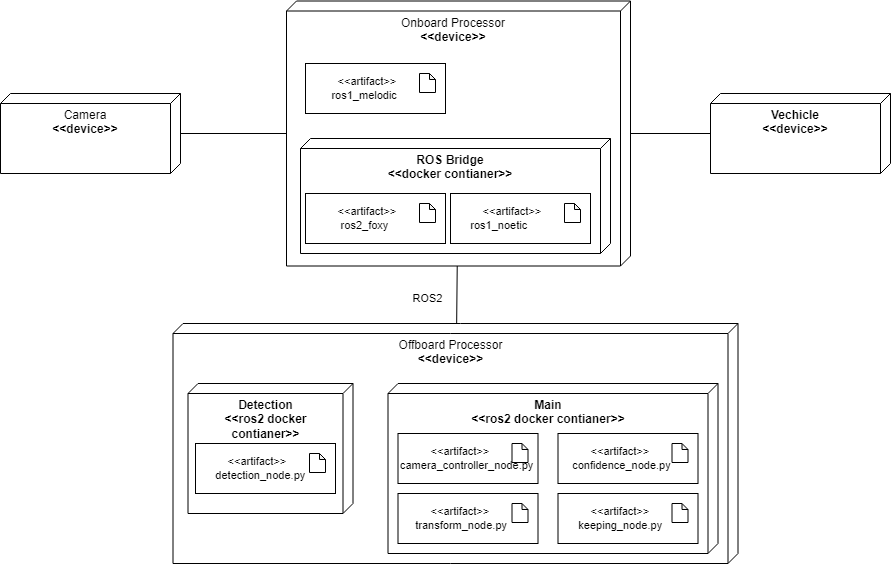
\includegraphics[width=6in]{deployment_uml}
	\caption{UML Deployment Diagram of the System}
	\label{fig:deployment}
\end{figure}

\subsubsection{Software Architecture}
From a software perspective, the system can be grouped into two categories: primary subsystems, which represent major workflows in the system, and secondary subsystems, which exist only to assist the primary subsystems with their workflows but are separate components.

The two primary subsystems in our project are the Detection and the Keeping \& Control subsystems. The Detection subsystem receives raw image data from the camera and determines the vehicle location within a lane, and sends this data to the Keeping \& Control subsystem. The K\&C subsystem interprets the lane data and produces movement commands to adjust the course of the vehicle. The two subsystems are discussed further in section 3 of this proposal.

Additionally, there are several secondary subsystems in our project. These secondary subsystems are the camera controller, the lane transformer, and the lane confidence subsystems. The camera controller is responsible for capturing the image feed from the camera mounted on the vehicle, and then supplying that to the detection node. The purpose behind this is to separate the detection module from the actual camera to remove any dependency issues. Additionally, we have a lane transformer subsystem which takes the data detected by the lane detection system and transforms it into a birds-eye view image of the lane data. The purpose of this is to simplify the operations of the primary subsystems and make it such that the primary subsystems can each be tested better in isolation. Lastly, we have the lane confidence node which assists with handling when a lane disappears from view. Its purpose is to keep track of lanes while they're present and ignore lanes that only appear for a singular frame, and extend lanes into new frames when they disappear spontaneously.

\subsubsection{Physical Architecture}

The physical architecture for the system is a distributed system with four significant hardware components: the camera, the onboard processing unit with ROS configured, the external processing unit with ROS configured, and the hardware/simulation for controlling the vehicle wheels. First, the camera sensor(s) captures the image data and sends that data to the onboard ROS environment. The onboard processor holds multiple different versions of ROS to allow communication with ROS2 nodes on the processors local network, allowing for it to communicate with an external laptop with stronger computing power. This laptop contains the software architecture described in section 1.4.1, broken down into two separate docker containers: one for the detection subsystem, and one for all the other subsystems. After the external processing has performed all the necessary calculations and generated a movement command, the movement command is sent back to the onboard processing unit which is then forwarded to the simulation or robot to execute the commands.

\subsection{Overview of Remainder of Report}

The remainder of the report will begin with Chapter 2, which will tie the project back to the Carleton Engineering project. It starts by outlining the health and safety concerns present as part of the project. Then, it will detail how the team exhibited the professionalism that is expected of engineering practitioners. The tools and systems used and project management skills demonstrated will also be discussed. Afterwards will be a quick discussion of how this project relates to each of the participants engineering disciplines. The section will conclude with an overview of the individual contributions made by each member of the team in both the report and the project as a whole.

Following the Engineering Project chapter will be chapter 3, which will focus on the work plan for the project. It will include the updated work breakdown structure, followed by a responsibility matrix, an activity network, and a Gantt chart. Then, a table will detail all of the costs and any special components that were required for the project. Lastly, the risk analysis table developed at the start of the project will be reviewed.

Following the work plan will be a highlight of the two primary subsystems for the project, the Detection subsystem and the Keeping \& Control subsystem. Each subsystem will have its requirements defined. Then, the technologies and methods important to the subsystem will be discussed. Following that, the considered solutions to the subsystem will be compared and the chosen path for that subsystem will be explained. The software architecture for that subsystem will be explained, followed by an explanation as to how the subsystem was implemented and subsequently evaluated.

After the explanation of the subsystems will be a section that will discuss how all the individual subsystems were designed to fit together, and then how the system as a whole was evaluated.

Lastly, the report will conclude with a reflection done by the group which will highlight the successes of the project, the significant changes from the proposal, and the group's reflections on what went wrong and what we would have done differently.

\section{The Engineering Project}

\subsection{Health and Safety}
For most of the development process, work was completed remotely and involved exclusively software development. As a result, there were no significant health and safety concerns that arose during the better part of development. However, as the project moved into the testing phase, potential saftey risks became apparent. The team made sure to follow all safety guidelines when working with the HiWonder JetAcker, and made sure to always have a spotter when the vehicle was in motion. Additionally, the team made sure to always have someone on standby to kill the program, stopping all commands to the JetAcker. The team also made sure a fire extingushier was nearby in case of spontaneous combustion of the JetAcker battery.

\subsection{Engineering Profesionalism}

The team used their experience from ECOR 4995 to a satisfactory extent during the performance of the project. The foremost principles from this course which we made sure to follow were effectively working as a team, and ensuring sustainability in our system.

For starters, the team did a great job at effectively cooperating. At the start of the project, the team got together and worked to best define what our objectives were for the project. After we understood the project sufficiently, we made sure that each member of the team had a clearly defined role. We also made sure to have clear and open communication with each other in case there were any issues that arose, allowing us to progress with little friction from each other.

In regards to legal and ethical obligations, the team ensured that all usage of libraries and open source projects was in compliance with license agreements and all aforementioned usage was properly cited. The team also did a great job at making sure that the work was sustainable for future projects. We understood at the start of the term that our project may be used by future engineering projects, so a major part of our work was focused on making our project as accessible as possible. This ensures the sustainability of our work by allowing improvements and extensions to be made.

\subsection{Project Management}
One of the goals of the engineering project is real experience in working on a long-term team project. Students should explain what project management techniques or processes were used to coordinate, manage and perform their project.

The way that we approached the development of our system was focused on an agile development cycle. The purpose of this is because while we were confident with our ability to work on the project, we understood that there was a lot of risk involved in what we were trying to do. Because of that, we couldn't set fixed goals and plan too far ahead and were forced to be flexible with deadlines and accomplishing goals. In order to properly keep track of all the required tasks and objectives, we used the project management service "ClickUp", explained in more detail in Chapter 3, which allowed us to easily track what had to be done, what dependencies existed in tasks, and track the progress on our timeline.

\subsection{Justification of Suitability for Degree Program}
In this section, students should explain how the project
relates to the degree program of each group member.

This project relates significantly to the degree of the students involved as each student is taking Software Engineering. The development of this system is entirely software based, and focuses on using many important software engineering concepts such as but not limited to project management, real-time systems, embedded systems, and machine learning.


\subsection{Individual Contributions}
This section should carefully itemize the individual contributions of each team member. Project contributions should identify which components of work were done by each  individual. Report contributions should list the author of  each major section of this report.

\subsubsection{Project Contributions}

Curtis:
\begin{itemize}
	\item CLRNet setup and configuration
	\item Docker setup and configuration
	\item CARLA setup and configuration
\end{itemize}

Robert:
\begin{itemize}
	\item ROS2 configuration
	\item Configuring JetAcker
	\item Confidence system
\end{itemize}

Ian:
\begin{itemize}
	\item Communication between subsystems
	\item Handling CLRNet outputs
	\item Line transformation system
\end{itemize}

Liam:
\begin{itemize}
	\item Controller setup and evaluation
\end{itemize}


\subsubsection{Report Contributions}
Curtis:
\begin{itemize}
	\item Abstract
	\item Chapter 1
	\item Chapter 4.1
	\item Chapter 6
	\item LaTeX Template
\end{itemize}

Robert:
\begin{itemize}
	\item Chapter 1
	\item Chapter 5
	\item Chapter 6
\end{itemize}

Ian:
\begin{itemize}
	\item Chapter 1
	\item Chapter 2
	\item Chapter 6
\end{itemize}

Liam:
\begin{itemize}
	\item Chapter 1
	\item Chapter 4.2
	\item Chapter 6
\end{itemize}

\section{Work Plan}

\subsection{Work Breakdown Structure}

\begin{figure}[H]
	\centering
	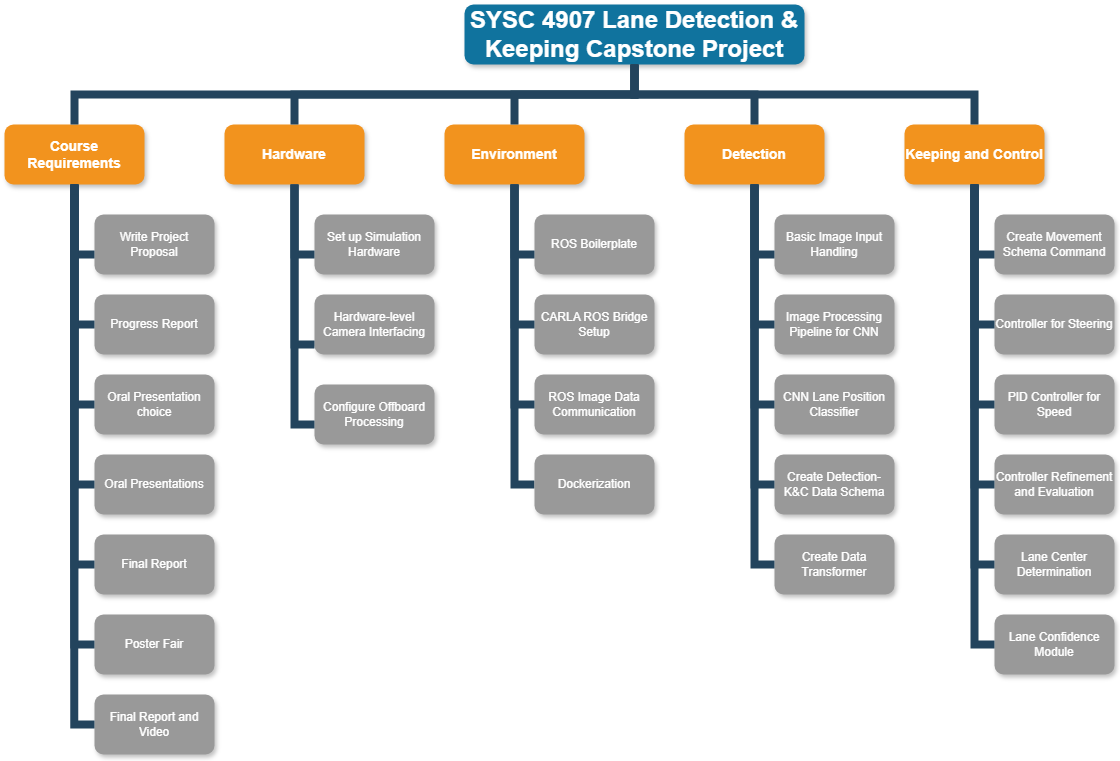
\includegraphics[angle=90,height=9in]{wbs}
	\caption{Project Work Breakdown Structure}
	\label{fig:wbs}
\end{figure}

\subsection{Responsibility Matrix}
\begin{table}[H]
	\centering
	\begin{tabular}{|c | c | c | c | c | c |}
		\hline
		Step & Project Task                         & Curtis & Liam & Ian & Robert \\ [0.5ex]
		\hline
		1    & Project Proposal                     & R      & R    & R   & R      \\
		\hline
		2    & Progress Report                      & R      & R    & R   & R      \\
		\hline
		3    & Oral Presentation                    & R      & R    & R   & R      \\
		\hline
		4    & Final Report Draft                   & R      & R    & R   & R      \\
		\hline
		5    & Poster Fair                          & R      & R    & R   & R      \\
		\hline
		6    & Final Report and Video               & R      & R    & R   & R      \\
		\hline
		7    & Set up Simulation Software           & R      &      &     &        \\
		\hline
		8    & Configure Offboard Processing        & R      &      &     &        \\
		\hline
		9    & ROS1-ROS2 Bridge                     &        &      &     & R      \\
		\hline
		10   & JetAcker Mesaging Configuration      &        &      &     & R      \\
		\hline
		11   & ROS Boilerplate                      &        &      &     & R      \\
		\hline
		12   & CARLA ROS Bridge Setup               & R      &      &     & S      \\
		\hline
		13   & ROS Message Types                    &        &      & R   &        \\
		\hline
		14   & Dockerization                        & R      &      &     &        \\
		\hline
		15   & Basic Image Input Handling           & R      &      &     &        \\
		\hline
		16   & Image Processing Pipeline for CNN    & R      &      &     &        \\
		\hline
		17   & Data Perspective Transformation      &        &      & R   &        \\
		\hline
		18   & Lane Confidence Module               &        &      &     & R      \\
		\hline
		19   & Controller for Steering              &        & R    &     &        \\
		\hline
		20   & Controller Refinement and Evaluation &        & R    &     &        \\
		\hline
		21   & Lane Center Determination            &        & R    &     &        \\
		\hline
	\end{tabular}
	\caption{Responsibility Matrix of Major Project Components and Tasks}
	\label{tab:WorkBreakdown}
\end{table}

\subsection{Project Network}

\begin{figure}[H]
	\centering
	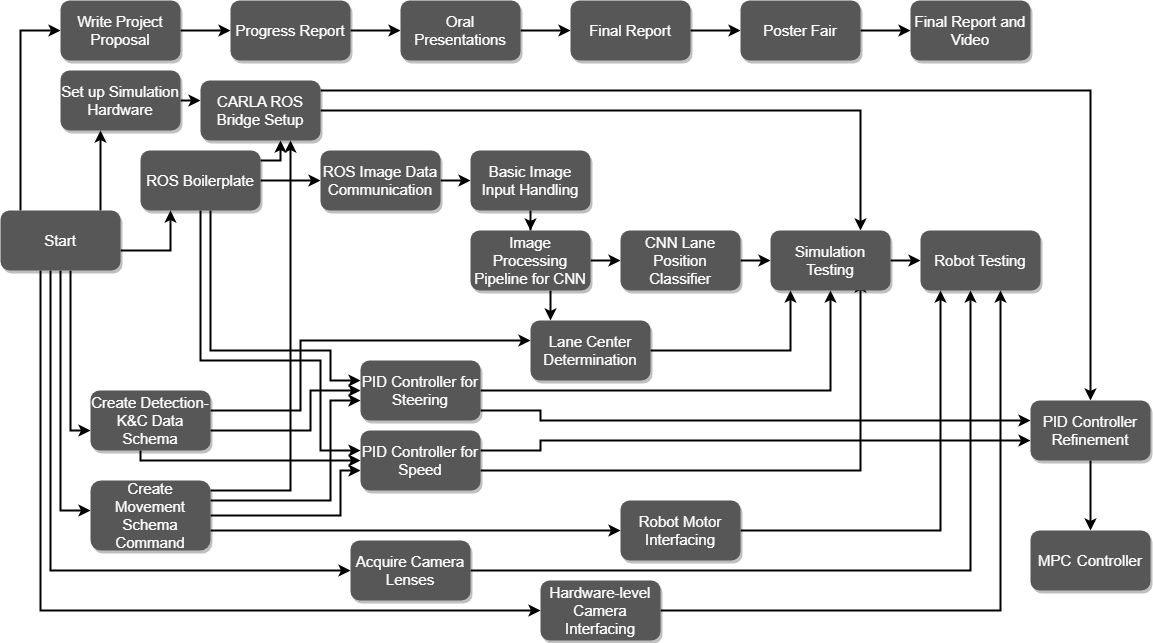
\includegraphics[angle=90,height=9in]{activity}
	\caption{Project Activity Network}
	\label{fig:activity}
\end{figure}

\subsection{Gantt Chart}

\begin{figure}[H]
	\centering
	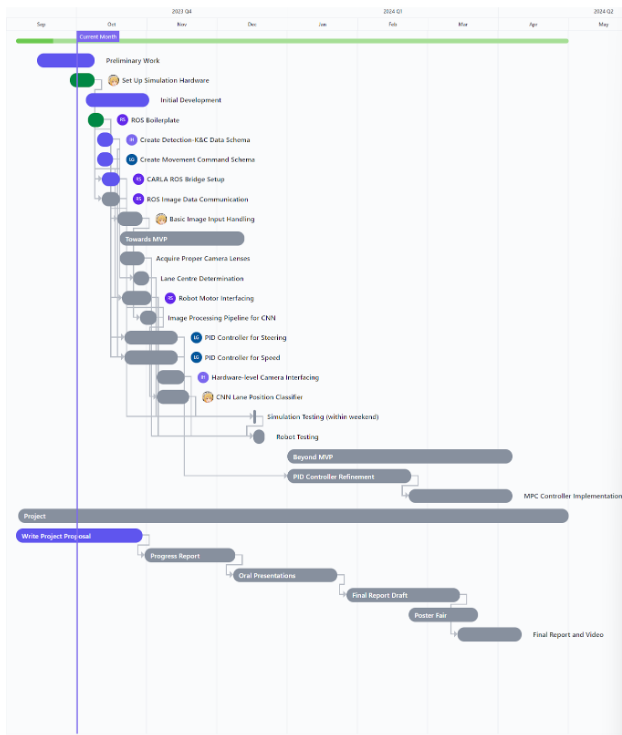
\includegraphics[angle=90,height=9in]{gantt}
	\caption{Gantt Chart of Project Tasks Over Time}
	\label{fig:gantt_chart}
\end{figure}

\subsection{Costs, Special Components and Facilities}
\begin{table}[H]
	\centering
	\begin{tabular}{@{}lp{0.5\linewidth}l@{}}
		\toprule
		\textbf{Item}     & \textbf{Description}                                                                                                                 & \textbf{Cost}                \\ \midrule
		HiWonder JetAcker & A robot that can have cameras configured onto the frame and respond to movement commands                                             & \$0 (Provided by Department) \\ \midrule
		Simulation Server & A computer running Ubuntu Linux, capable of running the CARLA Simulation software that can be accessed remotely for testing software & \$0 (Provided by Department) \\ \midrule
		SD Card           & An SD card for increasing the storage size of the HiWonder JetAcker                                                                  & \$30                         \\ \bottomrule
	\end{tabular}
	\caption{Extra materials purchased for this project and their associated costs.}
	\label{tab:costs}
\end{table}

\subsection{Risk Analysis}

In order to perform the risk analysis, the risk levels and meaning have to be identified. Table \ref{Table_risk_level} highlights the matrix that determines the overall risk level based on the probability of an event occurring and the impact it has on the success of the project. Table \ref{Table_risk_meaning} highlights the impact of the risk level and the appropriate steps to take for properly mitigating next.

\begin{figure}[H]
	\centering
	\begin{minipage}{.45\textwidth}
		\centering
		\begin{tabular}{|p{0.7in}|p{0.55in}|p{0.55in}|p{0.55in}|p{0.55in}|}
			\cline{1-5}
			\multicolumn{2}{|l|}{\multirow{2}{*}{RISK LEVEL}}                   & \multicolumn{3}{|l|}{\makecell{PROBABILITY of the event                                 \\ occuring}} \\ \cline{3-5}
			\multicolumn{2}{|l|}{}                                              & Low                                                     & Moderate & High               \\ \cline{1-5}
			\multirow{3}{0.8in}{SEVERITY of the event on the project's success} & Low                                                     & VERY LOW & LOW    & MEDIUM    \\ \cline{2-5}
			                                                                    & Moderate                                                & LOW      & MEDIUM & HIGH      \\ \cline{2-5}
			                                                                    & High                                                    & MEDIUM   & HIGH   & VERY HIGH \\ \cline{1-5}
		\end{tabular}
		\caption{Risk Level Matrix for Risk Analysis}
		\label{Table_risk_level}

	\end{minipage}%
	\hspace{0.1\textwidth}%
	\begin{minipage}{.45\textwidth}
		\centering
		\begin{tabular}{|@{}l|p{0.5\linewidth}|}
			\toprule
			Risk Level & Description                                                                                                               \\ \hline
			Very Low   & Very low risk, does not require any significant plans for mitigation                                                      \\ \hline
			Low        & A preliminary study on a plan of action to recover should be performed and documented                                     \\ \hline
			Moderate   & A significant risk. A plan of action to recover should be made in advance.                                                \\ \hline
			High       & A very significant risk that warrants considering a change in the project to address, or a plan of action should be made. \\ \hline
			Very High  & An unacceptable risk. The project should be changed to address this risk.                                                 \\ \bottomrule
		\end{tabular}
		\caption{Risk Level Meaning}
		\label{Table_risk_meaning}

	\end{minipage}
\end{figure}

At the beginning of the project, five risks were identified as being the most prominent issues that the team might run into over the course of the project. These risks were identified as the following: Neural Networks / ML is too complicated, Hardware not powerful enough, Scope Creep, Future Integration Challenges, and Software Version Incompatibility.

\textbf{Neural Networks / ML is too complicated}

The first risk for the project was whether the neural network/machine learning present in the lane detection would be too complicated for the team to handle. This risk was identified as a low probability, as some members of the team have prior experience designing neural networks and the problem domain means that there is a lot of reference material to draw on. Additionally, this risk was given a high severity since failure to properly construct a neural network would render the "Lane Detection" portion of the project impossible. As a result, this risk presented an overall moderate risk level for the team. The plan of action for this error would be if the neural network is too complex for the team to achieve, an algorithmic approach would be used as those are simpler to design than a neural network.

Unfortunately, this identified risk did occur during the development of the project. Despite the teams experience and the available resources, it proved to be too difficult to design our own convolutional neural network. However, further research into an algorithmic approach also proved challenging since the algorithmic approaches appeared to be more difficult than the neural network approach. In order to address this problem, the team instead opted for the use of a pre-existing CNN, CLRNet. This CNN proved to satisfy the requirements that our own neural network would need, and as a result the team could move forward with the rest of the project.

\textbf{Hardware is not Powerful Enough}

The second identified risk for the project was whether the hardware for the robot would be powerful enough. Since at the beginning of the project we did not have the proper technical specifications of the robot nor the technical requirements for the system to run, we were unsure if the final product could run on the robot. The chances of this were identified to be moderate since we knew there was a chance of this occurring, but thought it wouldn't be too likely. For severity, we identified this problem to be a moderate severity because the hardware should still be capable of running the neural network, but it would run it much slower than expected. As a result, the risk level identified with this risk was determined to be moderate. The plan of action for this risk was to instead make use of a distributed computing system, where a laptop would connect to the vehicle remotely and perform all the intensive action there.

As with the first risk, this identified risk also occurred during the development of the project. The HiWonder JetAcker proved to lack numerous hardware requirements to have the project run entirely on it, and as a result a distributed approach had to be used. There were many problems with setting up the distributed network though, since the JetAcker proved to have poor documentation and technical issues that made it difficult to properly distribute. However, despite the complications that were presented this risk was properly managed.

\textbf{Scope Creep}

Another identified risk with the project is a risk that is present in most development projects: scope creep. Scope creep occurs when proposed features keep getting added to the list of tasks to do to the point where there is too much work to get done and the team fails to address some of the most important tasks. For our team, we identified that the probability we encounter scope creep to be rather low, as following the projects proposal no new features will begin to be implemented until after all other performable work has been accomplished. Furthermore, the risk of scope creep to the overall success of the project was identified to be low since even if the team does accidentally start adding more to the project scope, additional features can easily be dropped. Since the risk level of this risk was identified to be very low, no major plans had to be designed. However, the plan for the project would be to try and accomplish a minimum viable product(MVP) as soon as possible so that new features can only be brought on once the core functionality has been implemented.

Over the course of the project, we did not encounter any issues with scope creep. The team did a good job of focusing on what needed to be done, and new features were only ever considered after individuals were left with nothing else to do. This risk was properly handled.

\textbf{Future Integration Challenges}

Since future projects might be building on this project, a significant risk is that of future integration challenges. While documentation and code readability will be prioritized, the time constraints put on the project could lead to quick solutions to problems that may not be easily read by future teams integrating our system with other autonomous driving systems. Given the amount of uncertainty in general with the project, it is moderately likely that this problem is encountered by the end of the projects development. However, even though it is quite likely to happen it is unlikely to affect the severity of this project since while integration with future self-driving systems is preferred but not critical to the project. Having software that is less interoperable with other services will not severely impact our system in itself. As a result, the overall risk level was determined to be low, and the plan of action to address this will be to always properly document code whenever code is submitted to the git repository.

As with the first two identified risks, this risk also occurred during our projects development. While this was a concern that was had throughout the project, the rate at which development was occurring led to poor documentation of many important procedures within the project. This problem was eventually addressed at the end of the project since the team spent time reviewing all the work performed, so future groups should still be able to use this repository with relative ease.

\textbf{Software Version Incompatibility}

The final significant risk identified at the beginning of the project was the potential for software version incompatibilities. This was deemed unlikely to occur since ROS 2, Ubuntu, Carla, and the Carla ROS bridge all have their own versions that are only compatible with specific versions of the others, but these are fairly clearly documented and problems should be straightforward to avoid. Furthermore, it was also deemed unlikely to affect the severity of the project since if an incompatibility between chosen versions is found and cannot be worked around, we could migrate to versions that are compatible, which may require changing Ubuntu versions but should not require redoing much work. Overall this risk was identified to be very low risk. No plan of action was identified because initial research showed that the versioning of all required systems was sufficiently stable that no further action would be required.

Unfortunately, this risk proved to be one of the largest problems encountered over the course of the project. While the software versions were compatible for the Carla, ROS 2, and Ubuntu portions, the version that existed on the JetAcker proved to be a very big problem. The result of this is discussed later, but to provide a short summary a member of the team spent several months dealing with an array of version incompatibilities to finally end with a functional system that works most of the time. For future reference, it should be noted that software incompatibility with this software should be considered a much larger risk than the team initially thought.


\section{Software Subsystems}

\subsection{Lane Detection}

The Lane Detection subsystem is responsible for detecting lane markers (road lines) in video frames sent from the camera
controller node and sending the locations of these markers on the video frames to the coordinate transformation node for
processing.

\subsubsection{Requirements}

Requirement from system-wide requirements:

\begin{itemize}
	\item \textbf{FR1}: 
\end{itemize}

Subsystem-specific requirements:
\begin{itemize}
	\item \textbf{FR1.1}: The subsystem should detect lane boundaries in a variety of driving conditions such as lighting and
	      road surfaces.

	      When operating a vehicle, Assisted Driving systems are expected to work in most driving conditions where a human driver
	      would reasonable be able to drive appropriately, such as night time or on roads with markings of varying colours.
	      While these environmental variations are often trivial to human drivers, they can pose significant issues for software
	      making decisions based on video data.
	      The subsystem must be able to work in different driving environments to avoid confusion by the driver.
	\item \textbf{FR1.2}: The subsystem should accurately infer lane boundaries that are somewhat obscured by objects on the
	      road such as other vehicles or concrete dividers.

	      In driving scenarios, it is not uncommon for lane markers to be partially obscured by other objects in the field of view
	      of the driver.
	      Cars on the road from busy traffic or passes can block direct vision of road lines, along with debris, dividers and any
	      other solid object.
	      Drivers are able to recognize these lines, but primitive detection algorithms may not make the distinction that two disjoint
	      line segments on an image belong to the same road line.
	\item \textbf{NFR1.1}: Real-time Processing: The subsystem must process video input fast enough to output lane location data
	      at a rate of no less than 10 frames per second.

	      Real-time processing is critical for a system that controls a vehicle moving at high-speeds along a road such as a highway.
	      While the curvature of high-speed roads is often slight to allow drivers to maintain control of their vehicles, the
	      system needs to be able to react to these changes quickly to maintain a smooth path at the centre of its lane as it drives.
	\item \textbf{NFR1.2}: Generic Input Handling: The subsystem must be able to accept video input that originated from any
	      class of video device.

	      One of the main goals of this project is that the system remain as hardware-agnostic as possible, and can be adapted for
	      different vehicle types and infrastructures with little modification.
	      In order to maintain this principle, the detection subsystem must decouple itself from any specific video capture hardware or
	      simulator that it ingests data from as we develop the system, such that future groups and developers can continue to work
	      on the system with different hardware or in different simulators.
	\item \textbf{NFR1.3}: The subsystem must accept and produce data on channels that can be accessed by external and/or future code.

	      This system is a starting point for the Lane Detection project for future groups to improve upon in later years.
	      In addition, future groups may be tasked with combining different autonomous driving systems into a single vehicle that provides
	      varying self-driving functionality.
	      The data ingested and generated by this subsystem must be made accessible such that other developers in the future have the
	      ability to hook into this subsystem and potentially redirect input/output to/from other systems for an improved self-driving
	      experience.
\end{itemize}


\subsubsection{Technologies and Methods}
~\\
\underline{Line Detection:}

The backbone of the detection subsystem lies in its use of computer vision and machine learning to identify lane markers in video
frames.

Computer vision is the field of study that deals with the development of algorithms and techniques for enabling computers
to interpret and understand visual information from images or videos.
While humans are good at making use of visual information, computers need to rely on these complex algorithms to turn image
data into usable information to act on.
While the term ``computer vision'' covers a broad spectrum of topics, commonly used computer vision techniques include video
processing, object recognition, face detection and augmented reality.
The ultimate goal of computer vision research is to enable machines to perceive and understand the visual world in a way that
is similar to or surpassing human vision.
This has numerous applications in fields such as robotics, autonomous vehicles, security systems and medical imaging, among
others.

Machine learning, a subset of artificial intelligence, is a rapidly growing field that focuses on developing algorithms and
models that enable computers to learn from data and make predictions or decisions based on that data without explicit programming
to do so.
At its core, machine learning enables algorithms to recognize patterns and relationships in datasets, allowing systems to adapt
and improve their decision-making abilities as they're exposed to more information.
This process, known as ``training'' a machine learning model, mimics the way in which humans learn, albeit at a much faster pace
and with a focus on specific tasks for each system and model.
The performance of machine learning models can be evaluated using various metrics, such as accuracy, precision, recall and F1
score.
Neural networks are a subset of machine learning algorithms inspired by the structure of biological neural networks in the human
brain.
They consist of interconnected nodes or artificial neurons organized into layers, with each layer processing input data using
mathematical functions and passing it on to the next layer.
The increase in complexity of these networks makes them more computationally expensive to train and run, but they can also yield
more high-level insights on large, complicated sets of data.

Due to the computationally expensive operations performed by a majority of machine learning programs, a computer's GPU is often
used for operating on machine learning models, rather than its CPU.
This is because while CPUs are better optimized for sequential execution of tasks, GPUs are designed to run a large number of
operations in parallel, making the hardware better suited to run the computations required for most machine learning applications.
However, since GPUs are primarily designed with graphics in mind, a software interface is required to use the GPU for
general-purpose computation.
NVIDIA provides the CUDA (Compute Unified Device Architecture) Toolkit \cite{CUDA} to allow developers to interface with its
GPUs for general-purpose computational tasks.
A similar stack, ROCm, is provided by AMD for use with its Radeon series of GPUs. \cite{ROCm}
\\~\\
\underline{Confidence}

The line detection system is not perfect. The exact position of the lines can fluctuate from frame to frame, and lines sometimes disappear briefly before being picked up again. To account for this, a system was designed to take past line data into account when deciding where lines are. This system works by maintaining a list of confidence lanes, which consist of a list of lines that are considered to be a part of the same lane and a confidence value between 0 and 1 that represents how confident the system is that the lane exists. Every time a new set of lines are detected, the system tries to match each one to an existing confidence lane by comparing the position of the line to the average of all the stored lines in each confidence lane. If it is close enough to one, it is added to that confidence lane's list, the oldest one is removed, and the confidence is increased. If it does not match anything, a new confidence lane is created with it as the only element in the list. After all lines have been processed, any confidence lanes that have not had a line added to them have their confidence decreased, and all confidence lanes with a high enough confidence have all their stored lines averaged and sent as output. The goal of this system is to smooth out the fluctuations in detected lines. The average of multiple past lines should reduce the side-to-side movement of the detected line, while the confidence aims to prevent lines from immediately disappearing from the output if they fail to be detected for a few frames.

The confidence system also includes some transformations to normalize the line data. This works by taking all the points that form a line, clipping off a portion at the top towards the horizon, matching a polynomial to what is left, and replacing the original irregular points with evenly-spaced points along the y-axis on this polynomial. Doing this makes operations like averaging and matching lines much more straightforward, since the system can expect to find points at specific y-values and average those. The line detection system struggles towards the horizon, so these points have to be removed before matching the polynomial. This portion of the system should probably be separated out into its own node to improve separation of concerns and make it easier to make changes and improvements to it.

Work on the confidence system began near the end of the semester, and it is not yet complete. The bulk of it is done, but there are still a few issues to iron out before it is useful. Clipping off the portion of the initial line near the horizon is not correctly implemented, resulting in the created polynomials being incorrect and turning the entire output into garbage.
\\~\\
\underline{Messaging and Data Transformations:}

The main transformation peformed on the lane data is a perspective transformation. A perspective transformation is a geometric transformation which can be applied to an image or list of points on a plane, to correct or modify its perspective \cite{CarletonHomography}. Perspective transformations can be used to correct distortions in an image or modify the viewpoint that an image is perceived at.
Homography refers to a transformation that maps points from one plane to another. In computer vision applications, homography is often used to describe the relationship of two images taken of the same scene, from different perspectives. Homography is useful for perspective transformations because it retains proportionality of the points within the image. To perform a perspective transformation, a homography matrix must be calculated. A homography matrix is a 3x3 matrix which describes the perspective transformation between two planes.
The first step of a typical method for generating a homography matrix is to identify sample points in the source image which form a polygon whose proportions are known, irrespective of how they may appear in the image. This is often done by identifying a quadrilateral within the source image which is known to be rectangular. For example, if an image contains a tile floor with rectangular tiles, the four corners of a tile may be used as the source points. The angles between these points are known to be 90 degrees, so the corresponding coordinates in the transformed image can be determined. From these source and destination points, the homography matrix may be generated and used the image or list of points within the image to complete the perspective transformation. Figure \ref{CarletonTransform} gives an example perspective transformation. The source points in the source image are chosen, shown on the left, and their corresponding points on the destination image are shown on the right.
\begin{figure}
	\centering
	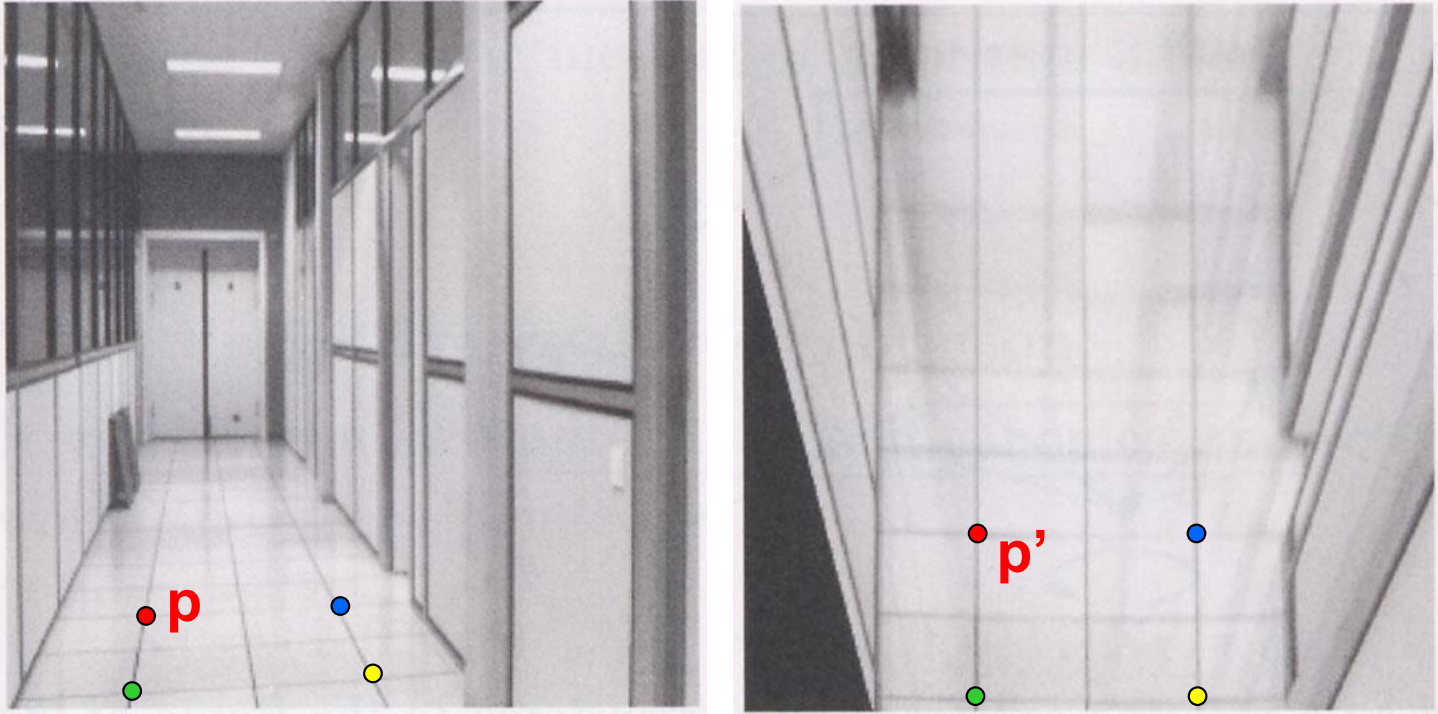
\includegraphics[width=6in]{transform_carleton.png}
	\caption{An example of a perspective transformation \cite{CarletonHomography}.}
	\label{CarletonTransform}
\end{figure}

When it comes to publishing lane data messages to ROS topics, some configuration is required to ensure compatibility with the underlying ROS messaging functionality. ROS messages are defined in a .msg file, which specifies the message type and fields. The message type is the name of the message, and the fields are the data that the message contains. To publish this data to a ROS topic, the data must be converted to a ROS message type \cite{ros_documentation}. For sending lane data, a custom message type must be defined in a .msg file. This message type must contain the data that is to be sent, and the data must be converted to this message type before being published to the ROS topic. In regards to our system, the lane data needing to be published is contained in a multidimensional array. ROS provides an interface for sending multidimensional arrays where a schema must be defined and this schema is used for processing the array into a message that can be published to a ROS topic \cite{ros_multi_array}. Another option for sending lane data involves flattening the data into a one dimensional array of \texttt{float32} values. This transforms the data into a compatible message type which can be published to a ROS topic. The data can then be reconstructed from the one dimensional array when it is received by another node. 


\subsubsection{Conceptualization}
\label{DetConcept}

\underline{Line Detection:}

There are many possible approaches to the problem of detecting road lines from a camera mounted in a vehicle.
In the planning phase of the project, we considered the use of detection techniques that did not use machine learning at all.
However, less complicated detection techniques can suffer from a lack of versatility.
This is an important aspect of lane detection, as vehicles are driven in a variety of environments that result in varying
levels of brightness, contrast and visibility of lane markers in video frames to be processed.

One considered approach to lane detection was the use of heavier image pre-processing and a Hough Transform to determine line
locations within video frames.
Hough Transforms work by representing lines in an image using a ``parameter space,'' where each point represents a set of
variables in a line or curve in the original image.
Lines and curves are detected in the image by find local maxima in the image after it has been transposed to the parameter space
for the task.
This can be seen in Figure \ref{HoughTransform}, where the parameters matching two straight lines are seen as white points in
the parameter space after the image is transposed.
After finding these maxima, the image can be converted back to its original coordinate space to find the detected lines and
curves.
This technique can be applied to the problem of lane detection, as the contrast between the black asphalt of the road and the
white or yellow painted lines can make good use of an appropriate parameter space for line and curve detection.

\begin{figure}
	\centering
	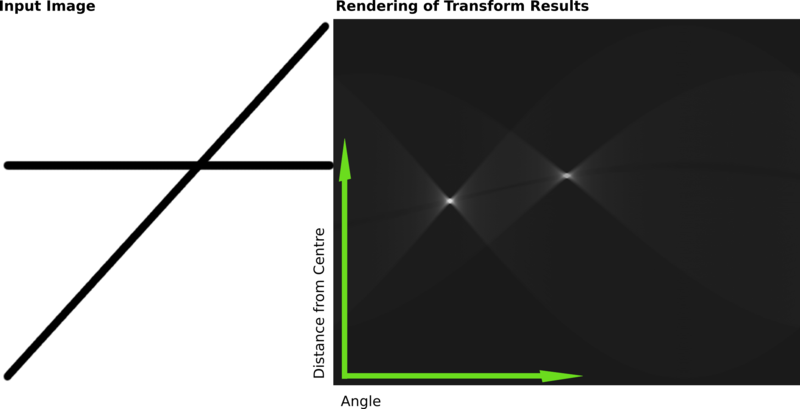
\includegraphics[width=0.5\textwidth]{Hough-example}
	\caption{An example of a Hough Transform used for line detection in an image.}
	\label{HoughTransform}
\end{figure}

One issue with the use of Hough Transforms is the changing contrast between road lines and the road surface, influenced by
factors such as wear, lighting conditions and other environmental variations.
In order to mediate this problem, different methods of image pre-processing were proposed in order to make the distinction
between road line and road surface as obvious as possible for the Hough Transform.
One of these proposed techniques was the conversion from the BGR colour space to the CIELAB (or La*b*) colour space.
La\*b\* is an alternative colour space in which colours are measured based on their \textbf{L}ightness, along with \textbf{a*} and
\textbf{b*} values corresponding to red-green and blue-yellow axes \cite{Mclaren2008}.
The rationale behind using the La*b* colour space is that as seen in Figure \ref{LabColourSpace}, yellow and white fall close
together in this space, meaning that light yellow and white road lines can be detected in a similar manner within the same space.

\begin{figure}
	\centering
	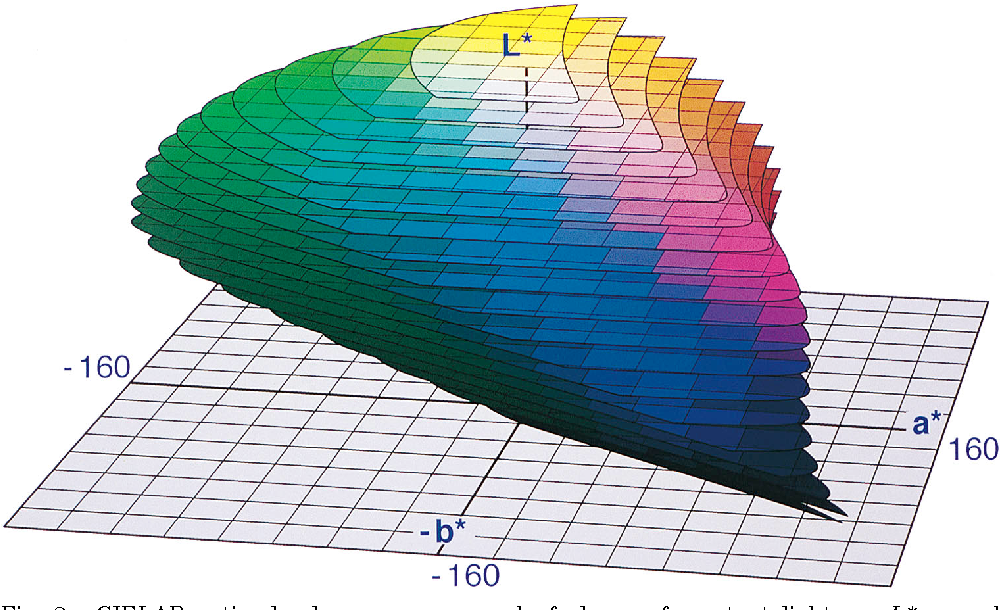
\includegraphics[width=0.5\textwidth]{Lab-colour-space}
	\caption{A visualisation of the different colours and their locations on the La*b* colour space.}
	\label{LabColourSpace}
\end{figure}

Ultimately, the use of these techniques was abandoned as while their implementation seems simple enough to understand and work
on, we feared the amount of extra work required to make the detection subsystem as usable in as many environments as possible
would grow too large, given the amount of time allocated for this project.

As an alternative to Hough Transforms, we looked into the use of machine learning for lane detection to leverage its versatility
in functioning in the dynamic environments a lane keeping system would experience in a vehicle as it drives.
Unlike Hough Transforms, which rely on predefined rules and parameters for the specific problem space, machine learning models
can be trained on large amounts of diverse data, making them flexible and capable of accommodating changes in road conditions
and lighting.

The TuSimple Lane Detection Benchmark\cite{TuSimpleBenchmark} was used as a metric to examine which machine learning approaches
to investigate for this project.
TuSimple is a Chinese company focused on making autonomous heavy-duty trucks for goods transportation.
They provide various benchmarks and large datasets of dashcam footage, which machine learning researchers can use to train and
test machine learning models for tasks such as lane detection and velocity estimation from image data. \cite{TuSimpleBenchmark}

Papers with Code is a database that provides open access to ``machine learning papers, code, datasets, methods and evaluation
tables''. \cite{PapersWithCode}
TuSimple uses Papers with Code to provide a leaderboard for their Lane Detection benchmark, listing papers that perform the best
on their datasets' test data, sorted by their accuracy or F1 scores.
As of writing this report, the top-performing models are listed in Table \ref{Table_TuSimpleBenchmark}, with their associated
papers, where applicable.
Out of the listed models, ones based on the CLRNet paper ranked best on both F1 scores and accuracy.
As these models were new and scored well, we saw this as an opportunity to implement bleeding-edge software into our system
to give it an edge for detecting lanes.

{\renewcommand{\arraystretch}{2}%
\begin{table}[]
	\centering
	\begin{tabular}{llllll}
		\textbf{Rank} & \textbf{Model}      & \textbf{Accuracy} & \textbf{F1 Score} & \textbf{Code?} & \textbf{Paper}         \\ \hline
		1             & CLRNet (ResNet-18)  & 96.82\%           & 97.89             & Y              & \cite{zheng2022clrnet} \\ \hline
		2             & CLRNet (ResNet-34)  & 96.9\%            & 97.82             & Y              & \cite{zheng2022clrnet} \\ \hline
		3             & CANet-L (ResNet101) & 96.76\%           & 97.77             & N              & \cite{yang2023canet}   \\ \hline
		4             & GANet (ResNet-34)   &                   & 97.71             & Y              & \cite{Wang_2022_CVPR}  \\ \hline
		5             & GANet (ResNet-18)   &                   & 97.68             & Y              & \cite{Wang_2022_CVPR}  \\ \hline
		6             & CLRNet (ResNet-101) &                   & 97.62             & Y              & \cite{zheng2022clrnet} \\ \hline
		7             & CANet-S             & 96.56\%           & 97.51             & N              & \cite{yang2023canet}   \\ \hline
		8             & GANet (ResNet-101)  &                   & 97.45             & Y              & \cite{Wang_2022_CVPR}  \\ \hline
		9             & CANet-M             & 96.66\%           & 97.44             & N              & \cite{yang2023canet}   \\ \hline
		10            & Oblique Convolution & 96.50\%           & 97.42             & N              & None                   \\ \hline
	\end{tabular}
	\caption{Top 10 TuSimple Lane Detection Benchmark models, March 2024.}
	\label{Table_TuSimpleBenchmark}
\end{table}

CLRNet (Cross Layer Refinement Network for Lane Detection) is a paper written by researchers from FABU.ai, a Chinese autonomous
driving development company, and Zhejiang University. \cite{zheng2022clrnet}
In this paper, a neural network algorithm known as a ``refinement network'' is used to accurately detect lanes on a road from an
image taken by a dashcam in a vehicle.
Refinement networks \cite{lin2016refinenet} are a type of machine learning technique in which objects are detected at a high
level and located with increased precision as the network decreases the scope further onto the detected objects.

A major advantage to the use of CLRNet is that the framework uses contextual information around an image to infer the positions
of lines even when they are not very visible on-screen.
For example, when another vehicle passes by the camera providing the video feed to CLRNet, it has little to no problems
accurately determining the location of the line behind the passing vehicle.
This coincides with requirement \textbf{FR1.2}, allowing the system to infer road lines that are obscured by objects in its field
of view.
Detected and inferred lanes also maintain a smooth shape, which is critical in our navigation system as we want to minimize
jitter introduced by jagged lines caused by errors in the detection subsystem.
\\~\\
\underline{Messaging and Data Transformations}
The two main tasks of the Messaging and Data Transformations subsystem are to process the lane data into a format that can be published to a ROS topic, and to perform any transformations on the detected lane markings before they are used by the K\&C subsystem.

After processing source images, the Detection module outputs lane markings as a list of lists, with each list representing a detected line, and each line consisting of several x,y coordinates denoting points on the line.  This formatting is useful for parsing the lane data, but cannot be easily included in a ROS message. ROS offers a functionality for publishing multi-dimensional arrays to topics; however, gaining familiarity with this functionality would be time consuming and the Python implementation for flattening the list of lines was not overly complex. Because of this, the decision was made to flatten the lane data before publishing it in a ROS message, and unflatten the lane data after it was received.

The mechanism used in the K\&C system, described in Section \ref{KCConcept}, requires data where the lane markings are plotted on a cartesian grid from a top-down perspective of the scene. The K\&C subsystem assumes the position of the camera to be at the origin, with lane markings extending in the positive y direction with lines to the left of the car having negative x coordinates and lines to the right of the car having positive x coordinates. These stipulations mean that after lanes have been detected from the source image, a perspective transformation must be performed to provide usable lane data to the K\&C subsystem for making steering adjustments. This design decision increases the risk of issues resulting from propagation of error or latency through the additional calculations, but it allows for the integration with the chosen solution for the K\&C subsystem. For future iterations of the system, the perspective transformation may become superfluous, depending on the specific controller used in those future iterations.


\subsubsection{Software Architecture}

The Lane Detection subsystem receives video frames from the Camera Controller node over a ROS topic, formatted as
\texttt{sensor\_msgs/Image} messages.
The subsystem uses CLRNet to detect the locations of road lines on the image, then sends this data over another ROS topic to the
Keeping \& Control node.
Using a ROS topic allows the actual line detection process to run asynchronously from the Camera Controller and Keeping \& Control nodes.
Since ROS nodes run on separate threads, this also allows other nodes to continue running during the computationally-expensive process
of line detection, whereas a synchronous approach would introduce hitching and delays that would be unacceptable in a real-time system
such as an autonomous vehicle.

\begin{figure}
	\centering
	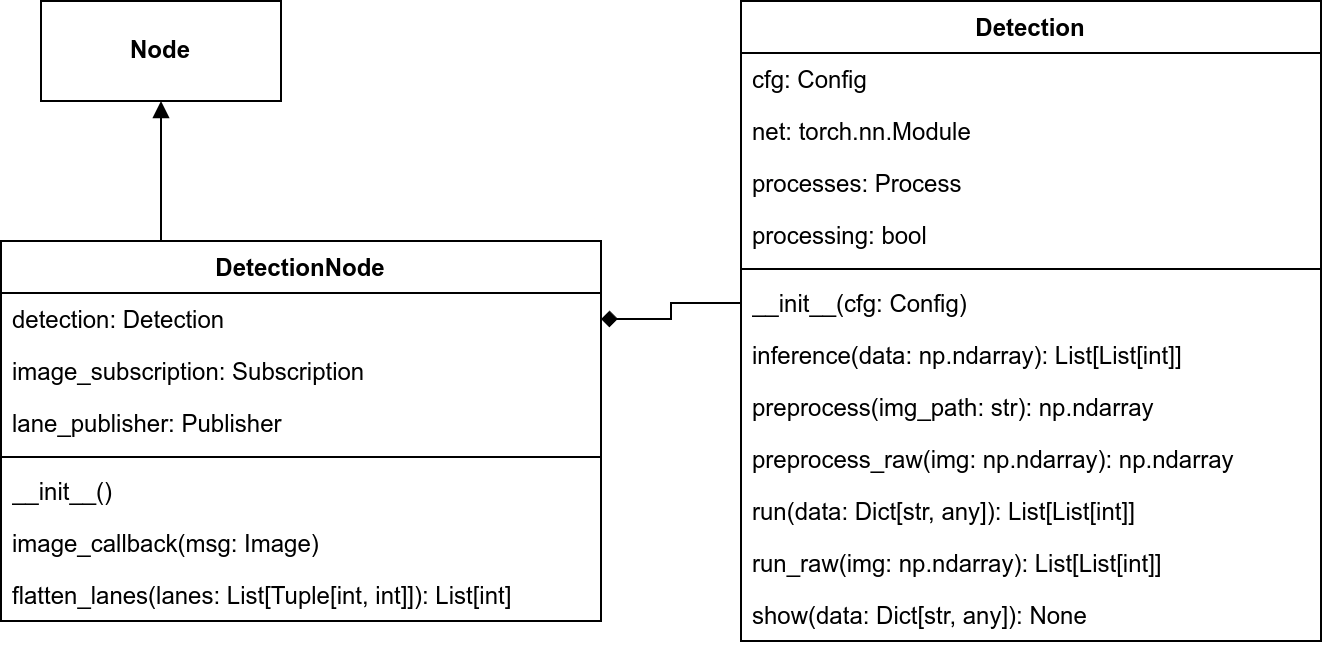
\includegraphics[width=0.7\textwidth]{Detection-UML}
	\caption{UML Class Diagram of the Detection Subsystem's ROS Node.}
	\label{Detection-UML}
\end{figure}

Since the actual lane marker detection process in this subsystem uses a neural network running on the GPU, the subsystem needs the
NVIDIA CUDA runtime to be installed in its environment.
The main system is based on the \texttt{ros-bridge} \cite{ROSBridge} Docker image, which does not have this toolkit installed.
To avoid bloating the environment on which the system runs, the detection subsystem runs in a separate Docker container based on the
\texttt{nvidia/cuda} Docker image, allowing it to interface with the host machine's GPU.
The networking stack in ROS2 allows nodes between Docker containers to communicate with one another without any additional configuration,
meaning that running lane detection in a separate container does not add any unnecessary complications in the system's architecture.

\subsubsection{Implementation}
\underline{Video Input}

The first step in implementing the lane detection aspect of the system is to set up a node that can accept video input
from a real or virtual camera.
This node, dubbed the Camera Controller, is responsible for capturing video frames from whichever source the system is
configured to use and outputting them to the Detection node as \texttt{sensor\_msgs/Image} messages over a ROS topic.
Since the system, in its state for this year, is designed to run on either the HiWonder JetAcker or a computer running
the CARLA simulator, the Camera Controller node is set up to accept video input from either the JetAcker's camera
via the \texttt{/camera/rgb/image\_raw} topic or from the CARLA-ROS bridge's simulated dashcam via the
\texttt{/carla/ego\_vehicle/camera/rgb/image\_raw} topic.
One of the main reasons for this design decision is to allow the system to be as hardware-agnostic as possible,
especially given that one of the initial cameras we were considering using for the JetAcker required a custom driver
to be installed on the system, and we wanted to minimize coupling between the system and the hardware it runs on.
\\

\underline{Video Preprocessing}

CLRNet expects images to be in a $800 \times 600$ resolution before processing, with a configurable \texttt{cut\_height}
parameter that determines how much of the image from the top is cropped before being fed into the network.
When CLRNet was initially trained on the TuSimple dataset, the images were cropped to remove the top 320 pixels in order
to remove irrelevant information from above the horizon line (not used in lane detection) from frames.
Since CLRNet is trained on dashcam footage, any additional preprocessing steps such as colour space conversion
may yield worse results than the original images, as the network is already trained to work with the colour space
provided by the dashcam.
\\

\underline{Lane Detection}

Using CLRNet for lane detection without re-training the model on the dataset is relatively simple.
TuRoad provides the LaneDet \cite{LaneDet} tool, a Python program that interfaces with different lane detection models
to detect lanes in images and show the results in a window or save them to a file.
While the tool is designed to be a command-line utility, it can be easily modified to be used as a Python module
to be integrated into the Detection node by replacing the file path input with input provided by the Camera Controller node.
LaneDet also does not have explicit support for CLRNet, but the model can be loaded into the tool by modifying some of
the dependency imports to load code from the CLRNet Python interface instead of the default model interface in the repository.
Code in \texttt{detection.py} makes the necessary imports to code which was borrowed from LaneDet to load the
CLRNet model and run it on arbitrary video frames which are passed in from the Camera Controller node.
\\

\underline{Detection Results}

Once CLRNet has been run on a video frame, the model provides output formatted as a list of lanes, where each lane is
a series of points on the lane.
Each point is a tuple of decimal numbers ranging from 0 to 1, representing the x and y coordinates of the point with
respect to the input image's dimensions.
Upon a successful detection cycle, the Detection node makes the required formatting adjustments to the data before sending
it to the Keeping \& Control node.
\\


\underline{Messaging and Data Transformations}


The first challenge addressed by the Messaging and Data Transformations module is the reformatting of lane data into a ROS compatible data type. Publishing messages to ROS topics first requires the use of message interfaces. The interfaces for the system are defined in the \texttt{/ros2\_ws/src/lane\_interfaces} directory. The interface for sending lane location data is named LaneLocation and consists of five attributes, stamp, frame\_id, lanes, row\_lengths, and img\_shape. The stamp and frame\_id attributes are of type string and provide the timestamp for the message and filename for the image associated with the lanes respectively. These two attributes are not currently used by the system, but were added to include metadata that may become useful for future features. The lanes attribute is an array with elements of type float32. This attribute contains the data representing the lanes detected for an image. The row\_lengths attribute is an array with elements of type int32 and stores the number of points for each detected line. The image\_shape attribute is also an array with elements of type int32 and stores the dimensions of the image, to be used in the perspective transformation.

The lines detected by the Detection subsystem are outputted as a list of lists, with each list representing a detected line, and each line consisting of several x,y coordinates denoting points on the line, as described in Section \ref{DetConcept}. Since the object is a multidimensional list, it must be restructured to allow for it to be published to a ROS topic. To account for this, the list was flattened by iterating through each list of points, and separately adding the $x$ and $y$ components to a list. The points remain ordered as they were in the original list.

\[ 1: \{[(x1, y1), (x2, y2), \cdots], [(x3, y3), (x4, y4), \cdots ], [(x5, y5), (x6, y6), \cdots], \cdots \} \]
\[ 2: \{x1, y1, x2, y2, x3, y3, x4, y4, x5, y5, x6, y6, \cdots\} \]

List 1 depicts the structure of the lanes before flattening, and List 2 depicts the lanes after flattening. The implementation for the flattening and unflattening methods is contained in the \texttt{line\_transformations.py} file. For unflattening the data, the process is reversed by iterating through the flattened list and adding the $x$ and $y$ components to a list of points. The points are then grouped into lists of points, with each list representing a detected line. 

\begin{figure}
	\centering
	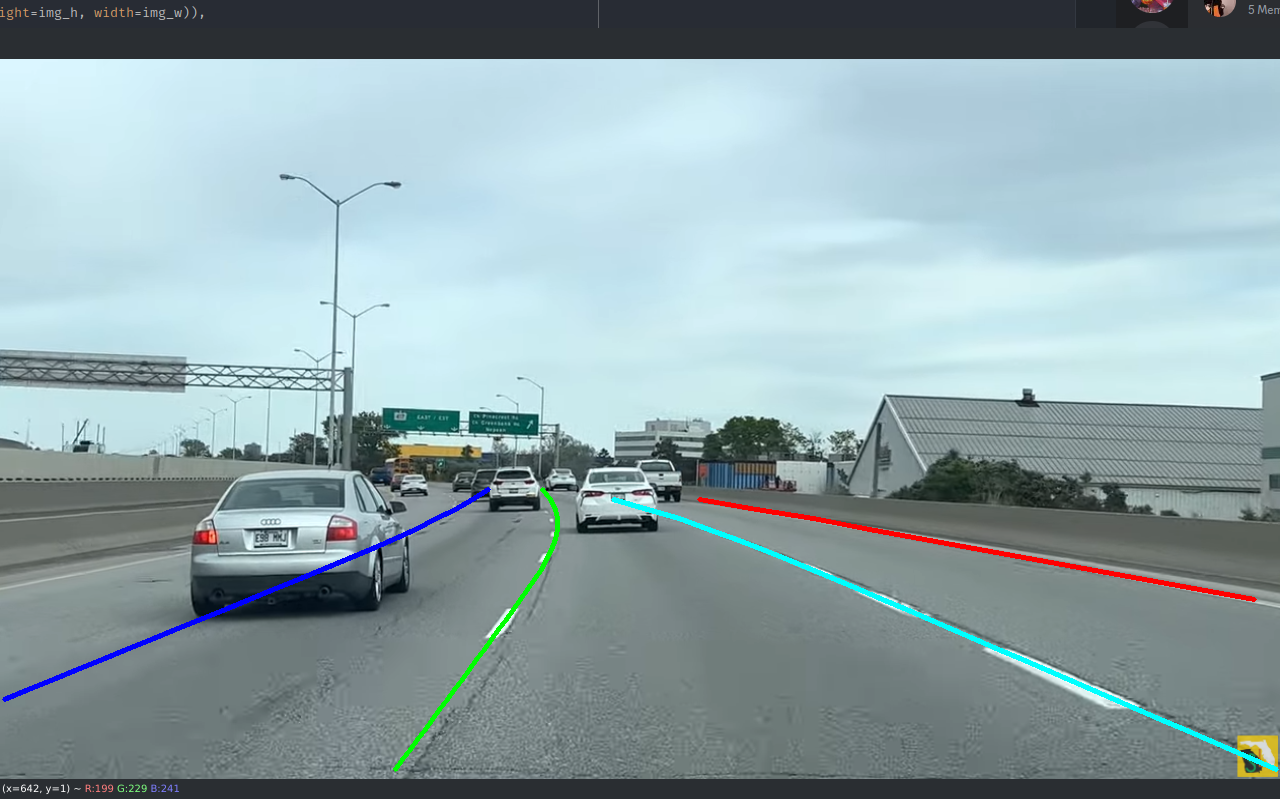
\includegraphics[width=0.7\textwidth]{ikea_lines.png}
	\caption{An example image with detected lane markings, before perspective transformation.  \textit{Modified from} \cite{ikea_image}}
	\label{ikea_lines}
\end{figure}

\begin{figure}
	\centering
	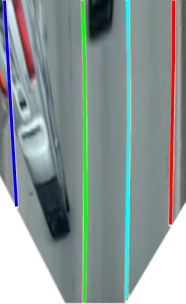
\includegraphics[height=0.6\textwidth]{top_down_ikea.png}
	\caption{The example image from Figure \ref{ikea_lines}, after perspective transformation.  \textit{Modified from} \cite{ikea_image}}
	\label{transformed_ikea}
\end{figure}

The next challenge tackled by the Messaging and Data Transformation module was to transform the lanes from the first person camera perspective to a top down representation of the scene. In the \texttt{lanes\_to\_birds\_eye()} method in \texttt{line\_transformations.py} file. This method takes lane data as input and converts each point into a corresponding point in the top donw perspective. To obtain the homography matrix for the transformation, the vanishing point of the image is calculated to allow a source trapezoid to be defined \cite{johncmitchell}. The source trapezoid is used in conjunction with a destination rectangle and both are passed into the \texttt{cv2.getPerspectiveTransform()} method from Python's OpenCV library. The homography matrix is then used to transform each point in the lane data using the \texttt{cv2.perspectiveTransform()} method. The transformed lane data is then returned to be published to a ROS topic. Figure \ref{ikea_lines} shows an example image with detected lane markings, and Figure \ref{transformed_ikea} shows the same image after perspective transformation. The images themselves are not transformed within the actual implementation and are shown in the figures to improve understanding. 


\subsubsection{Evaluation}

\begin{table}[]
    \centering
    \captionsetup{justification=centering,margin=2cm}
    \begin{tabular}{@{}lrrrrrrr@{}}
        \toprule
        \textbf{Method} & \textbf{Backbone}        & \textbf{F1 (\%)} & \textbf{Acc (\%)}  & \textbf{FP (\%)} & \textbf{FN (\%)} \\ \midrule
        
        SCNN~\cite{pan2018spatial} & VGG16 & 95.97 & 96.53  & 6.17 & \textbf{1.80} \\
        
        RESA~\cite{zheng2021resa} & ResNet34 & 96.93 & 96.82 & 3.63 & 2.48  \\
        
        PolyLaneNet~\cite{tabelini2021polylanenet}  & EfficientNetB0 & 90.62 & 93.36 & 9.42 & 9.33 \\
        
        E2E~\cite{yoo2020end}  & ERFNet  & 96.25  & 96.02  & 3.21 & 4.28 \\
        
        UFLD\cite{qin2020ultra} & ResNet18 & 87.87 & 95.82 & 19.05 & 3.92 \\
        
        UFLD\cite{qin2020ultra}  &  ResNet34 & 88.02 & 95.86  & 18.91 & 3.75 \\
        
        LaneATT\cite{tabelini2021keep} & ResNet18 & 96.71 & 95.57 & 3.56 & 3.01 \\
        
        LaneATT\cite{tabelini2021keep} & ResNet34 & 96.77 & 95.63 & 3.53 & 2.92 \\
        
        LaneATT\cite{tabelini2021keep} & ResNet122 & 96.06 & 96.10 & 5.64 & 2.17 \\
        
        FOLOLane\cite{qu2021focus} & ERFNet & 96.59 & \textbf{96.92} & 4.47 & 2.28 \\
        
        CondLaneNet\cite{liu2021condlanenet} & ResNet18 & 97.01 & 95.48 & 2.18 & 3.80 \\
        
        CondLaneNet\cite{liu2021condlanenet} & ResNet34 & 96.98 & 95.37  & 2.20 & 3.82 \\
        
        CondLaneNet\cite{liu2021condlanenet} & ResNet101 & 97.24 & 96.54 & \textbf{2.01} & 3.50 \\
        \midrule

        \textbf{\methodname} & ResNet18                                & \textbf{97.89}                                 & 96.84                                 & 2.28                                 & 1.92  \\

        \textbf{\methodname}  &     ResNet34                & 97.82                                 &  96.87                                 & 2.27                                 &  2.08    \\

        \textbf{\methodname} & ResNet101                               & 97.62                                 &  96.83                                 & 2.37                                 & 2.38    \\ 
        \bottomrule
    \end{tabular}
    \caption{CLRNet researchers' comparison of state-of-the art models during development. (Source: CLRNet \cite{zheng2022clrnet})}
    \label{tab:tusimple_main}
\end{table}


% \begin{table}
%     \begin{center}
%     \resizebox{0.5\textwidth}{!}{%
%             \begin{tabular}{@{}lrrrrrrr@{}}
%                 \toprule
%                 \textbf{Method} & \textbf{Backbone}        & \textbf{F1 (\%)} & \textbf{Acc (\%)}  & \textbf{FPS} & \textbf{MACs (G)} & \textbf{FP (\%)} & \textbf{FN (\%)} \\ \midrule
                
%                 SCNN~\cite{pan2018spatial} & VGG16 & 95.97 & 96.53 & 7.5 & - & 6.17 & 1.80 \\
                
%                 RESA~\cite{zheng2021resa} & ResNet34 & 96.93 & 96.82 & - & - & 3.63 & 2.48  \\
                
%                 PolyLaneNet~\cite{tabelini2021polylanenet}  & EfficientNetB0 & 90.62 & 93.36 & 115 & 1.7 & 9.42 & 9.33 \\
                
%                 E2E~\cite{yoo2020end}  & ERFNet  & 96.25  & 96.02  & - & - & 3.21 & 4.28 \\
                
%                 UFLD\cite{qin2020ultra} & ResNet18 & 87.87 & 95.82 & 312.5 & - & 19.05 & 3.92 \\
                
%                 UFLD\cite{qin2020ultra}  &  ResNet34 & 88.02 & 95.86 & 169.5 & - & 18.91 & 3.75 \\
                
%                 LaneATT\cite{tabelini2021keep} & ResNet18 & 96.71 & 95.57 & 250 & 9.3 & 3.56 & 3.01 \\
                
%                 LaneATT\cite{tabelini2021keep} & ResNet34 & 96.77 & 95.63 & 171 & 18.0 & 3.53 & 2.92 \\
                
%                 LaneATT\cite{tabelini2021keep} & ResNet122 & 96.06 & 96.10 & 26 & 70.5 & 5.64 & 2.17 \\
                
%                 FOLOLane\cite{qu2021focus} & ERFNet & 96.59 & 96.92 & - & - & 4.47 & 2.28 \\
                
%                 CondLaneNet\cite{liu2021condlanenet} & ResNet18 & 97.01 & 95.48 & 220 & 10.2 & 2.18 & 3.80 \\
                
%                 CondLaneNet\cite{liu2021condlanenet} & ResNet34 & 96.98 & 95.37 & 154 & 19.6 & 2.20 & 3.82 \\
                
%                 CondLaneNet\cite{liu2021condlanenet} & ResNet101 & 97.24 & 96.54 & 58 & 44.8 & 2.01 & 3.50 \\
%                 \midrule

%                 \textbf{\methodname} & ResNet18                                & 95.57                                 & \underline{3.56}                                 & 3.01                                 & \underline{250}                              & \underline{9.3} \\

%                 \textbf{\methodname}  &     ResNet34                & 95.63                                 & \textbf{3.53}                                 & 2.92                                 & 171                              & 18.0 \\

%                 \textbf{\methodname} & ResNet101                               & 96.10                                 & 5.64                                 & 2.17                                 & 26                               & 70.5 \\ 
%                 \textbf{\methodname}  & ERFNet                                & 96.10                                 & 5.64                                 & 2.17                                 & 26                               & 70.5 \\ \bottomrule
                

%             \end{tabular}
%     }

%     \end{center}
%     \caption{State-of-the-art results on TuSimple. For a fairer comparison, the FPS of the fastest method (\cite{ufsa}) was measured on the same machine and conditions as our method. Additionally, all metrics for this method were computed using the official source code, since only the accuracy was available in the paper.}

%     \label{tab:tusimple_main}

% \end{table}


Given the extensive evaluation performed on CLRNet by its authors, we used the results of their experiments described in
the CLRNet paper \cite{zheng2022clrnet} as a benchmark for its use in the system.
For one of its benchmarks, Zheng et el. used the TuSimple dataset to compare performance scores of the different implementations
of CLRNet to other state-of-the-art lane detection models.
CLRNet, using ResNet18 as a backbone, provides the highest F1 score out of all the models tested, with a score of 97.89\%.

In this case, the F1 score is a relevant metric to use for evaluating lane detection performance, as it measures both
the rate at which the model correctly detects lanes and the rate at which it correctly ignores non-lane features in the frame.
The former is important for ensuring the vehicle has a clear understanding of where its lane boundaries are, while the latter
is important for ensuring the vehicle does not make steering adjustments based on false positives derived from the video frame.

\subsection{Lane Keeping \& Control}
The Lane Keeping \& Control (K\&C) subsystem is responsible for taking in lane position data with relation to the vehicle, determining the best corrective action to take to steer the vehicle towards the center of its lane and execute the appropriate instructions to the hardware/simulation.

\subsubsection{Requirements}
Requirement from system-wide requirements:

\begin{itemize}
	\item FR2: Lane Following Precision. The system should maintain a deviation of no more than 0.45 meters from the center of its lane under normal driving conditions.

	      As stated earlier, the ability to precisely follow the center of the lane is a very important functional requirement of the system. The primary purpose of this subsystem is therefore to fulfill that functional requirement by creating a control system that given the position of the lanes with respect to the vehicle, will be able to precisely follow their path.

\end{itemize}
Subsystem-specific requirements:
\begin{itemize}


	\item FR2.1: Steering Control Stability. The control subsystem should aim to minimize the heading error of the vehicle.

	      An important part of self-driving cars is the stability of the steering. It is not desirable for the humans in the vehicle if the steering of the car is continuously changing direction and overcompensating, meaning that the control system must minimize the heading error associated with the steering.

	\item FR2.2: Control Frequency.
	      The subsystem must produce movement command updates at a frequency of 50Hz.

	      An important part of any real-time control system is that it must be able to reach deadlines. Additionally, a control system must exhibit continuous interaction with the environment which it is located within. To achieve these goals, the system must therefore be required to produce periodic movement commands that are frequent enough to give the appearance of continuous motion. The frequency of 50Hz was agreed upon by the group and the project supervisors as sufficiently frequent to represent continuous feedback from the control system.

	\item FR2.3: Closed Loop Properties.
	      The subsystem must produce movement commands using the most recent information available.

	      In control systems, there are usually two kinds of control systems: open and closed systems. Open control systems typically involve no feedback being provided to the control system between output commands, whereas closed loop systems are fed information which is to be used as part of the command generation. It is our intention to make the control system closed loop because it is important that the subsystem is continuously fed data about its positioning for subsequent commands.

	      However, one potential issue with a purely closed loop system is due to a timing concern. The rate at which lane data is received from the detection module may not be able to keep up with the rate of the desired control frequency defined in FR2.2. This means that there may be times which the system is required to produce an output without having received information about its position within the system, which represents an open control loop.

	      Therefore, it is important for our system to use as much closed loop properties as possible, and only rely on open loop properties when the latest data is not available.

	\item FR2.4: Output Attributes. The output commands produced by the subsystem must output the fewest parameters required for path execution.

	      One of the primary goals of the system is to be very easy to configure for new hardware environments. For the control system, this means that the system must be able to output movement commands that are easily interpretable for any hardware environment it might be in. This does not mean that it must automatically be compatible with every hardware setup, but it must provide sufficient information such that an adapter can be used to convert between the control systems movement command and the hardware's execution.
\end{itemize}


\subsubsection{Technologies and Methods}
The development of the K\&C subsystem requires the use of three primary technologies and software concepts.

For starters, the K\&C system will require the use of multi-threading. Multithreading is the process by which a system has multiple concurrent threads, a program in execution, running concurrently in parallel. There are several advantages of using multi-threading, including better performance due to being able to run tasks during I/O blocking time, greater scheduling flexibility, and it separates the concern of what a task does and when it does it. With respect to our system, multithreading will need to be used to have our PID processing run in parallel to receiving new system environments from the lane detection subsystem. Multithreading was instructed as part of the SYSC 3303 Introduction to Real Time Systems course offered at Carleton.

Another important methodology for this project is that of feedback control systems. These systems are control systems that incorporate comparing the measured variable with its target value and then manipulates the system to minimize this error\cite{intro_to_feedback_sys}. Feedback control systems are advantageous since the controller takes into account any unforeseen changes present in the system such as friction from the environment or older data such as from long input processing times, both of which are likely to happen with our system\cite{intro_to_feedback_sys}. These concepts are taught as part of the SYSC 3600 and SYSC 4505 courses offered at Carleton University. While these courses are not required as part of a Software Engineering degree, they can be taken as electives for students in Software Engineering and the project supervisors have experience with this concept that can be shared with the students.

Cars and car-like vehicles use an arrangement of linkages called an Ackermann steering geometry in order to steer effectively[17]. It allows for the wheels on the inside and outside of a turn to trace circles of different radii, preventing slipping. In systems that use Ackermann steering or something similar, the front wheels turn while the rear wheels remain in place. In contrast, robots like the JetAuto use mecanum wheels, which allow for omnidirectional movement. While this is a useful property for robots, we intend to use the JetAuto to evaluate the system’s capabilities for car-like vehicles. As such, this subsystem should be able to send commands to vehicles with mecanum wheels that result in Ackermann-like movement. While this concept was not explicitly taught as part of a software engineering degree at Carleton, the integration of hardware components with embedded systems relates to the practices discussed in SYSC 3310 Introduction to Real-Time Systems.

\subsubsection{Conceptualization}
\label{KCConcept}

There are many control loops that could be used to handle the lane keeping and control requirements for this sub-system. However, out of all these methods, there are three that have stood out for us as potential conceptual solutions.
\\

\underline{PID Controller:}

A PID controller is an error driven controller. This means it works by being fed a source of error, and outputs actions intended to minimize it. The output is calculated using three components: a proportional, a derivative, and an integral component.

First, the proportional component calculates an output value that is directly proportional to the source of error. The effect of the proportional controller on the output is typically a significant immediate reaction to the output of the device. Next is the derivative component, which calculates an output value using the derivative of the error at the current point in time. The derivative component in PID controllers is typically used as a means of dampening the oscillation in the source of error that arises from the proportional component. Lastly, the integral component works by outputting a value proportional to the total error up to the current point in time. Integral components are largely effective at reducing the steady state error of the system to ensure that it reaches the desired value faster.  Using the outputs of these three values, the PID controller adds them together and outputs a command that is intended to minimize the error, which then starts the next cycle of the PID controller\cite{pid_explanation}. Fig.\ref{fig:piddiagram} illustrates a diagram of a typical PID controller.\\

\begin{figure}
	\centering
	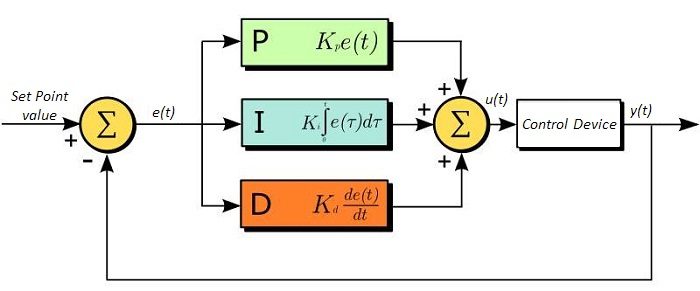
\includegraphics[width=4in]{PID2.jpg}
	\caption{Diagram of a Typical PID Controller}
	\label{fig:piddiagram}
\end{figure}

One of the things that makes PID controllers desirable is its tuning process. PID controllers only have three tunable constants, being the proportional constant \((K_p)\), the integral component \((K_i)\), and the derivative component \((K_d)\). After the PID controller is implemented, these three constants are then used to tune the system to a desired effect. \cite{pid_advantages}

The three main measurements used for evaluating a PID controller are the settling time, overshoot, and rise time. Within a PID controller, the settling time is typically defined as the time required to enter the 5\% error strip. The overshoot of the system is defined as the maximum amount by which the response overshoots the steady state value. Lastly, the rise time is typically defined as the time it takes for the controller to get from 10\% to 90\% of the steady state value. Each of these attributes are affected by the three constants in a PID controller, and the effect that each constant has on the overall controller can be found in Table \ref{tab:pidvals}.

\begin{table}[H]
	\centering
	\caption{Effect of PID Controller Characteristics Through Changing Constants \cite{pid_characteristics}}
	\begin{tabular}{|c | c | c | c | c |}
		\hline
		Increase in Constant & Rise Time    & Overshoot & Settling Time & S-S Error  \\ [0.5ex]
		\hline
		\(Kp\)               & Decrease     & Increase  & Small Change  & Decrease   \\
		\hline
		\(Ki\)               & Decrease     & Increase  & Increase      & Decrease   \\
		\hline
		\(Kd\)               & Small Change & Decrease  & Decrease      & No Changes \\
		\hline
	\end{tabular}
	\label{tab:pidvals}
\end{table}

The main advantage with a PID controller is its simplicity, both with designing and with tuning the controller. For starters, a PID controller is very simple to implement. PID controllers are not very technically complicated compared to other control schemes, and many PID controller packages already exist which could easily be used instead of creating a custom one. As a result, the only thing that needs to be determined is the source of the error for the system, and how the output affects the system. Additionally, PID controllers are very straightforward to tune. A PID controller only has three constants, all three of which have predictable effects on the performance of the controller.

Despite the advantages, there are numerous drawbacks to using a PID controller. For starters, the tuning of the controller can only be so effective. Since there are only three constants to tune, there is a much worse peak to the performance of the controller compared to more sophisticated models, such as the Model Predictive Control described next. Additionally, since the model is error driven it is very sensitive to noise in the error, especially with respect to the derivative component.
\\

\underline{Model Predictive Control:}

The MPC controller is a more sophisticated control system compared to the PID controller, with use in various industries and areas in academia.\cite{GARCIA1989335} It utilizes a model of the system, a cost function, and an optimization algorithm to determine the optimal strategy for minimizing error, which in this case is the distance between the car's centre and the centre of its lane.

One significant advantage of this controller is its potential for high accuracy when implemented effectively. The MPC controller takes a wider array of variables and information into account when making decisions, offering greater potential for improved performance metrics.

However, MPC comes with the drawback of increased complexity. Unlike a PID controller, which is relatively straightforward to set up and configure, implementing an MPC controller involves considering a larger set of variables and a model of the environment surrounding the system, making it more challenging during the initial stages of development.
\\

\underline{Stanford Mathematical Model (Stanley Controller):}

The Stanley controller is a model based controller that calculates its recommended trajectory by using the vehicles distance to the centre of the path and the heading error with the tangent line of the closest point. Most notably, it focuses on the trajectory of the vehicle with respect to the orientation of the front wheels as opposed to the entire vehicles body\cite{4282788}.

The Stanley controller is composed of two schemes that are used to model the vehicles motion. The first is the kinematic model, which works under the assumption that the vehicle has negligible inertia, focuses on the position and heading of the vehicle's front axis with respect to the centre of the lane. The second is the dynamic model which includes the additional inertial effects such as tire slip and steering actuation. These two models can be seen below in Fig. \ref{fig:stankine} and Fig. \ref{fig:standyna}.

\begin{figure}
	\centering
	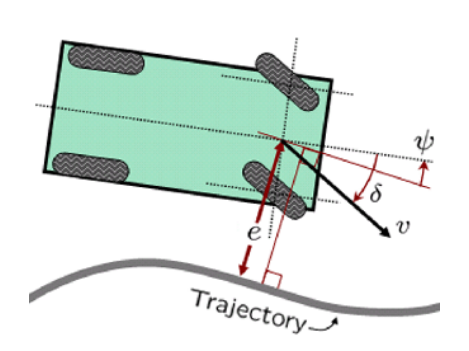
\includegraphics[width=4in]{stanley_kinematic}
	\caption{Kinematic Model of a Stanley Controller\cite{4282788}}
	\label{fig:stankine}
\end{figure}

\begin{figure}
	\centering
	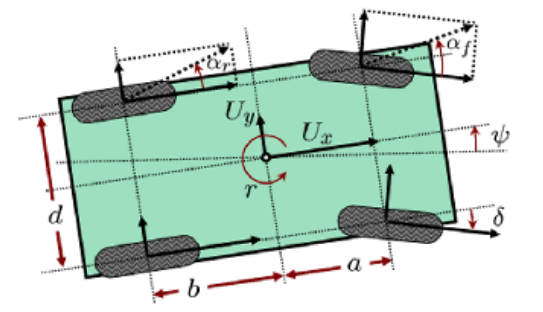
\includegraphics[width=4in]{stanley_dynamic}
	\caption{Dynamic Model of a Stanley Controller\cite{4282788}}
	\label{fig:standyna}
\end{figure}

The main advantage of the Stanley controller is that it can be very easy to implement, and can scale very well with complexity. The Stanley controller's two models allows for two different degrees of complexity within the model, ensuring that a simple approach can be used in addition to a more complicated model for further improvement. Additionally, the complexity of the kinematic model is not technically complex to implement.

However, a disadvantage with the control system is that the dynamic model is not interchangeable between environments. The dynamic model has a very strong relationship with the architecture of the vehicle, meaning that it is not particularly interchangeable to new systems.
\\

\underline{Chosen Solution:}

The original decision for which control system architecture to base the subsystem on was a PID controller. At that time, the two main control systems that were being considered was the PID controller and the MPC controller. Between these two options, it was significantly more difficult to try and implement the MPC controller due to the complexity associated with its implementation and the more complex theory associated with it. As a result, a PID controller was chosen as the starting point for development.

However, after having spent some time trying to implement the PID controller it was determined that the theory of how to integrate PID control within the system proved to be more complex than originally anticipated. Further research was conducted, and the team discovered the Stanley controller. This model proved to be significantly easier for the team to implement, and the disadvantages of the model being that it had a lot stronger coupling was negligible since we were more focused with getting any control system working. As a result, the decision was made to make this subsystem based on the Stanley controller.

\subsubsection{Software Architecture}

The Lane Keeping \& Control subsystem receives lane data from the Detection subsystem via a ROS topic using a publish-subscribe approach, allowing for asynchronous communication to accommodate different processing rates. The LaneDataListener component captures the lane position data and updates the LaneControl component. This component operates on a 50Hz timer, determining the optimal angle and velocity for the vehicle to stay centered in its lane. The output is formatted as an
\texttt{ackermann\_message/AckermannDrive} message,
a data type provided by ROS, and then published to a separate ROS topic. This data is subsequently utilized by either a hardware module (simulated or real) capable of responding to Ackermann steering signals, or a software component that interprets the Ackermann steering commands and converts them into a compatible format. Figures \ref{fig:control_class} and \ref{fig:control_sequence} further illustrate the architecture of the system.


\begin{figure}
	\centering
	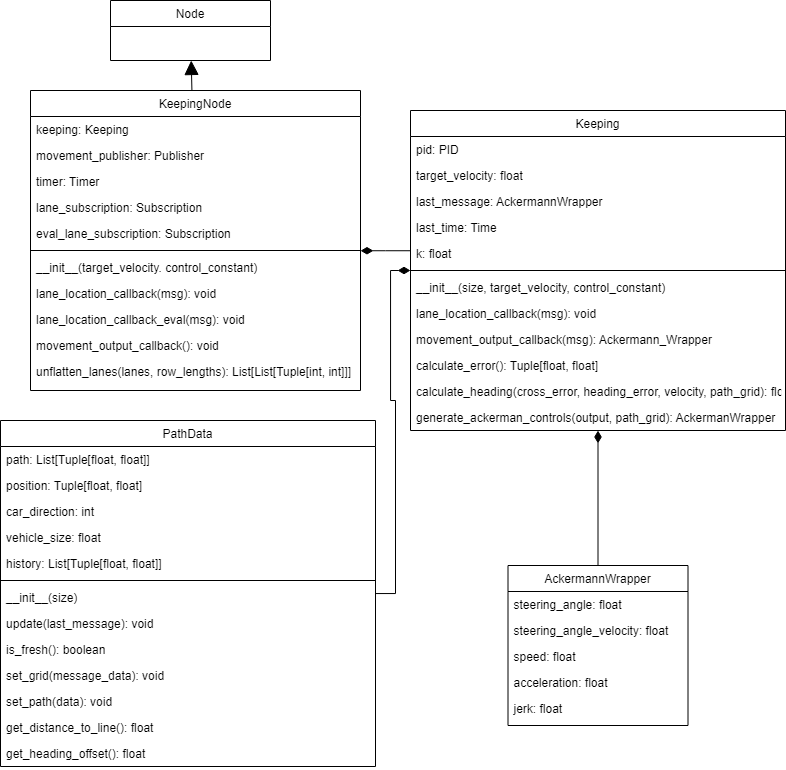
\includegraphics[width=0.7\textwidth]{KnC_diagrams}
	\caption{UML Class Diagram of the K\&C Subsystem}
	\label{fig:control_class}
\end{figure}

\begin{figure}
	\centering
	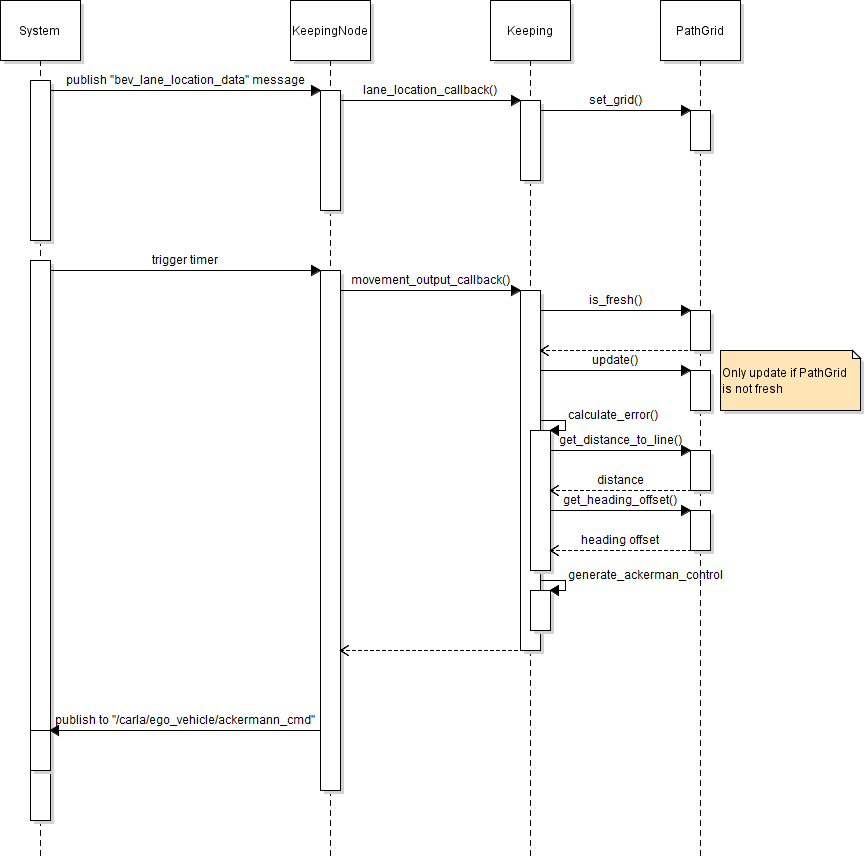
\includegraphics[width=0.9\textwidth]{KnC_sequence.png}
	\caption{UML Sequence Diagram of the K\&C Subsystem}
	\label{fig:control_sequence}
\end{figure}

The subsystem makes use of a proxy pattern for handling and sending requests. The reason for this is due to containerization issues. In order to run the ROS node, the system needs to actually run on ROS or else the "Node" package fails to properly import. The use of a proxy pattern here helps allows for the testing of files without the need for importing the ROS packages, allowing for more efficient development.


\subsubsection{Implementation}
\underline{Communication Schema}

The first step in building the K\&C subsystem was by establishing the communication schema between this subsystem and the adjacent control systems. This was imperative since without an idea of how each subsystem would communicate with this one, it would be impossible to start the development process. This meant identifying the correct input to the system, and the correct output from the system to the environment.

For the output of the system, the decision was made to use the built-in AckermannDrive message type that is already built into ROS. The reason for this was because it was already built into ROS, and was already integrated into the CARLA ROS Bridge which means it required less configuration to integrate the subsystem with CARLA. The AckermannDrive message asks for five parameters. The first parameter in the AckermannDrive message is the steering angle. This represents the desired steering angle that the vehicles front axis should be set to. The system will attempt to adjust the orientation of the wheels to that desired steering angle as quickly as possible. The second parameter is the steering angle velocity, which works in conjunction with the steering angle. This parameter specifies the maximum velocity that the yaw of the steering angle can achieve, where a zero represents no limit. This parameter is important as it prevents severe amounts of jerk with the steering, but it was not an important parameter for our system. The third parameter for the AckermannDrive message is the velocity. This represents the target velocity that the vehicle should aim to reach, to be achieved however the vehicle deems fit. The fourth and fifth parameters are the acceleration and jerk parameters, which set a maximum acceleration and jerk that the vehicle can achieve while attempting to adjust to the desired speed. The definition of this message type can be found in Fig. \ref{fig:ackermann}

\begin{figure}
	\centering
	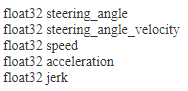
\includegraphics[width=0.3\textwidth]{ackeramnn_drive}
	\caption{Structure of the ROS AckermannDrive Message Type}
	\label{fig:ackermann}
\end{figure}

For the input to the system, a schema needed to be designed that allowed for a list of lane data points to be sent to the control subsystem. The first idea for this would be to have a list of list of tuples that contains the data points for each line. That is, a list of lanes where each lane is represented by a list of points, where each point is represented as a tuple. However, one problem that we had with this is that it was not the exact format that we thought that the detection subsystem would naturally produce. In research, it was determined that the output of the detection subsystem would more closely resemble the TuSimple schema which can be found in Fig. \ref{fig:tusimple_dataformat}. This is because we would be comparing the output of the detection to the TuSimple dataset, so our data would already be in this format. Furthermore, this format for the data is more efficient to send because it normalizes the data points by providing a list of Y-coordinates and each lane is instead represented by a list of X-coordinates, where points are generated by matching indexes. Due to the similarity with the TuSimple dataset output and the more efficient transformation method, this data scheme was chosen as the communication the subsystem would get from the detection subsystem.

\begin{figure}
	\centering
	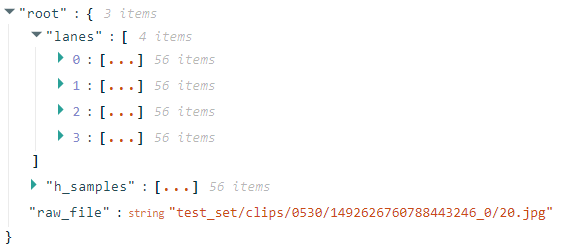
\includegraphics[width=0.6\textwidth]{tusimple_data_example}
	\caption{Example of the Structure of the TuSimple Dataset}
	\label{fig:tusimple_dataformat}
\end{figure}

\underline{Creating the PID Controller}

After the control schema was established, the next step was to create the PID controller. The PID controller was originally chosen as the control system due to its simplicity of design, so this represented the next hurdle for implementing this subsystem.

The first step in implementing the PID controller was actually creating the PID controller. In general, PID controllers are straightforward to create. Through the use of various tutorials and discussing PID controllers with fellow students, a functional PID controller was implemented. Afterwards, the PID controller was tested in a console environment to ensure that it worked as expected, and could theoretically be used for the control system.

The implementation of the PID controller can be found within our project
repository at \\\texttt{/lane-detection-keeping/ros2\textunderscore ws/src/lane\textunderscore nodes\textunderscore py/lane\textunderscore odes\textunderscore py/keeping/pid\textunderscore controller.py}
\\

\underline{Creating the Internal Map}

After the PID controller was implemented, the next step was creating an internal representation of the vehicle's environment. This is important for two reasons. For starters, having an internal representation of the environment would be essential in calculating the error that needs to be fed into the PID controller for it to work. Without an appropriate model of the environment available, it would be hard to determine the error and the control system would have a hard time properly steering. Additionally, since the rate at which lane data is produced is much slower than the rate at which the control system must enact movement commands, the system must be able to track roughly how far the vehicle has moved through its environment as it generates movement commands. Without this, the subsystem would not be able to achieve its output frequency of 50Hz.

The first step in implementing the internal map was to identify the path for the vehicle to follow. This means that in order for a model of its environment to exist, it must be created from the passed lane data from the detection subsystem. To do this, the internal map parses the lane data received from the detection and attempts to map each lane into a polynomial. The purpose of this is to smooth the lane curve to get rid of any jagged shapes that might appear in the lane lines. Through a mild amount of testing, a degree of 3 was chosen for the polynomial fitting. This is because the shape of curves is rarely straight enough for a degree of 1 or 2, and a degree of 4 or higher starts to suffer from overfitting which destroys the accuracy of the polynomial. After the lanes are turned into polynomials, the system identifies the closest lane that appears on each side of the origin by comparing the y-intercepts of the lanes. The system finds the smallest y-intercept above 0 and sets that as the left lane, and the lane with the largest y-intercept below 0 and sets that as the right lane. Then, it averages the polynomials for the two lanes to determine the centre of the two lanes, and stores that path as the centre lane for the vehicle to follow. Fig. \ref{fig:lane_center_determination} illustrates this process.

\begin{figure}
	\centering
	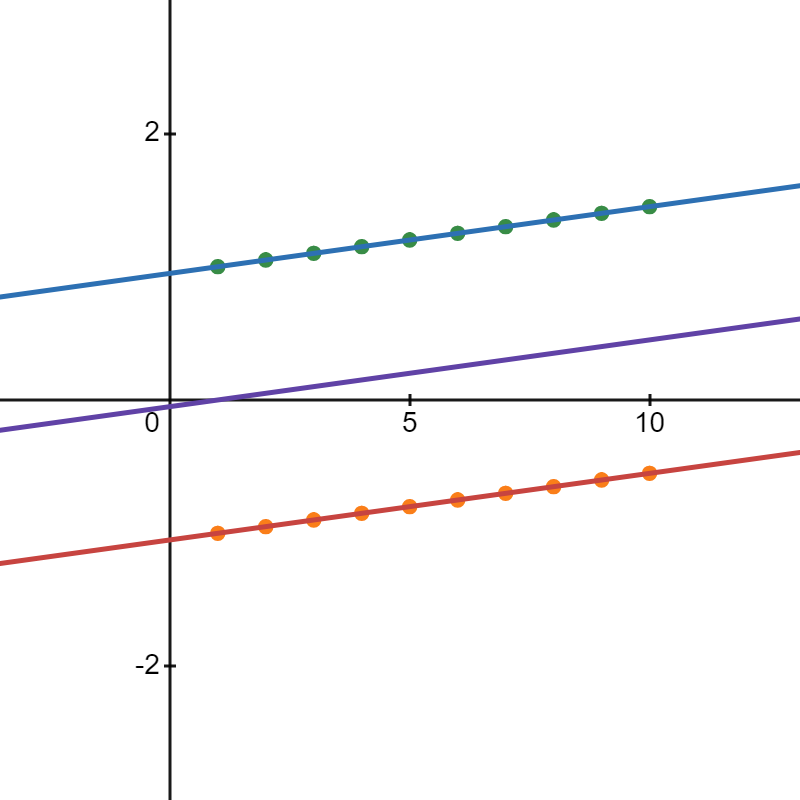
\includegraphics[width=0.7\textwidth]{lane_center}
	\caption{Calculation of the Center of the Lanes}
	\label{fig:lane_center_determination}
\end{figure}

The second step in implementing the internal map is to be able to predict where the vehicle is if no new lane data is received. This is important for the system because one of the requirements is to be able to use the latest available data for each command output, so its important that when the system is relying on old data it can predict where the vehicle moves between output commands. The first thing done to implement this was to set a flag on the internal grid called "fresh" which is set to true whenever a lane centre is configured, but then swapped to false after a movement command is generated. If the lane data is not fresh, the system will then update the position of the vehicle in the internal grid based on how much time has passed, and the last movement command enacted.

The steps for predicting the vehicles new position is done in four steps. The first step is to find the pivot point. An important part of Ackermann steering is that it works by having all the wheels oriented perpendicular to a singular pivot point. This means that given the last movement commands heading, we can take the distance between the axis and the angle of the heading to find the point which the vehicle will pivot around. Next, the system has to determine how far the vehicle actually travels. This is done by taking the time between the last movement command and the present, and multiplying it by the speed of the last movement command to get a distance. Afterwards, the number of radians travelled around with respect to the pivot point is calculated. Lastly, using the amount of radians that the system rotated about the pivot point the vehicles new position is calculated. Figure \ref{fig:internal_update_determination} provides a visual representation of the math. It should be noted that this method of predicting the vehicles location is not very accurate, as it works in an ideal world and simplifies a lot of the movement that is occurring.

\begin{figure}
	\centering
	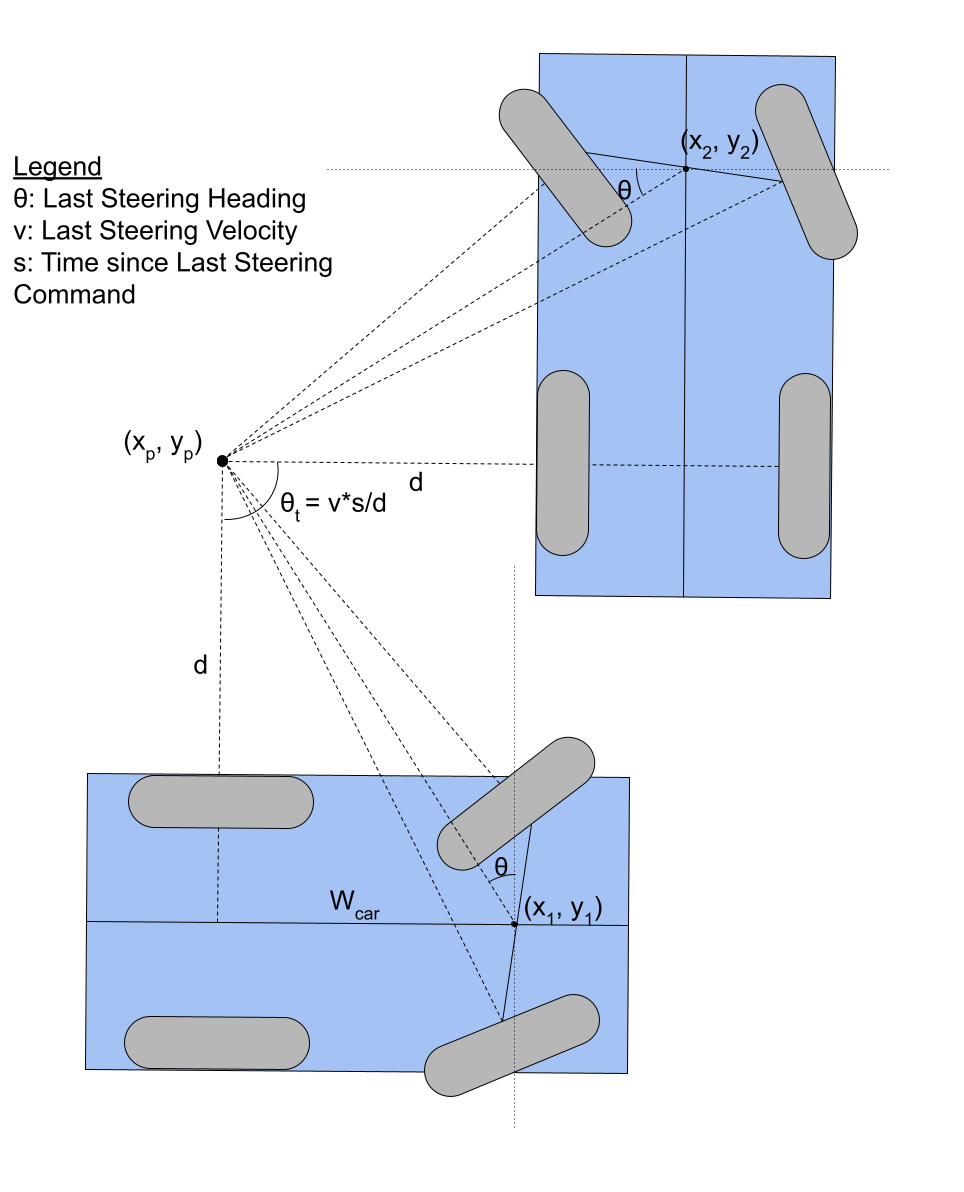
\includegraphics[width=5in]{update_description}
	\caption{Calculating the Vehicles New Position Between Cycles Without New Data}
	\label{fig:internal_update_determination}
\end{figure}

The full implementation of the internal mapping system can be found within the code repository at \texttt{/lane-detection-keeping/ros2\textunderscore ws/src/lane\textunderscore nodes\textunderscore py/lane\textunderscore odes\textunderscore py/keeping/robot\textunderscore path.py}
\\

\underline{The Problem with PID}

After having created the PID controller and the internal representation of the vehicle in its environment, it came time to putting these two components together to create a functional system. However, this proved to be a challenge. While the theory behind the use of a PID controller is very straightforward, a conventional PID controller works by taking a single source of error and outputting commands that are intended to minimize it. With respect to a system such as autonomous driving, its difficult to identify a singular source of error. For example, if we consider the source of error to be just the distance between the vehicles front axis to the centre of the lane and the output to represent the steering angle, then it becomes very easy for the vehicle to overcompensate its steering and start turning the opposite direction if the vehicle is too far away. On the other hand, if the source of error is the heading error of the vehicle then the vehicle will reach a parallel state with the centre of the lane and not be obliged to move closer to it. As a result, it proved difficult to identify an appropriate way to implement a single PID controller that can effectively include both of these errors in the PID algorithm. Furthermore, attempts to find implementations of PID controllers online for autonomous driving proved difficult and unhelpful, and a search for an alternative control system began.
\\

\underline{The Discovery of the Stanley Controller}

Further research conducted on simple control systems for autonomous driving led to the discovery of the Stanley Controller. This controller was originally designed in 2005 by Stanford University for autonomous driving in the 2005 DARPA Autonomous Driving Challenge, and works by using a mathematical model of the vehicles position to the centre of the lane and provides a means of effectively balancing the cross track error and the heading error of the vehicle at the same time, addressing the issues with implementing a PID controller. Since this control method looked functional and there was sufficient documentation from the control systems original page, the team worked to implement this control system instead.
\\

\underline{The Implementation of the Stanley Controller}

The Stanley controller primarily requires two sources of error to function.

First, it requires the heading error. This can easily be gathered from the control systems internal model of its environment by doing a few linear algebra calculations. The first step of this process is to identify the two closest points of the path from the internal model. These two closest points are then used to create a secant line from which the heading of the vehicle, which is stored within the model, is compared to in order to identify the heading error of the vehicle. A visual representation of this calculation can be found in Fig. \ref{fig:stanley_heading_calc}.

\begin{figure}
	\centering
	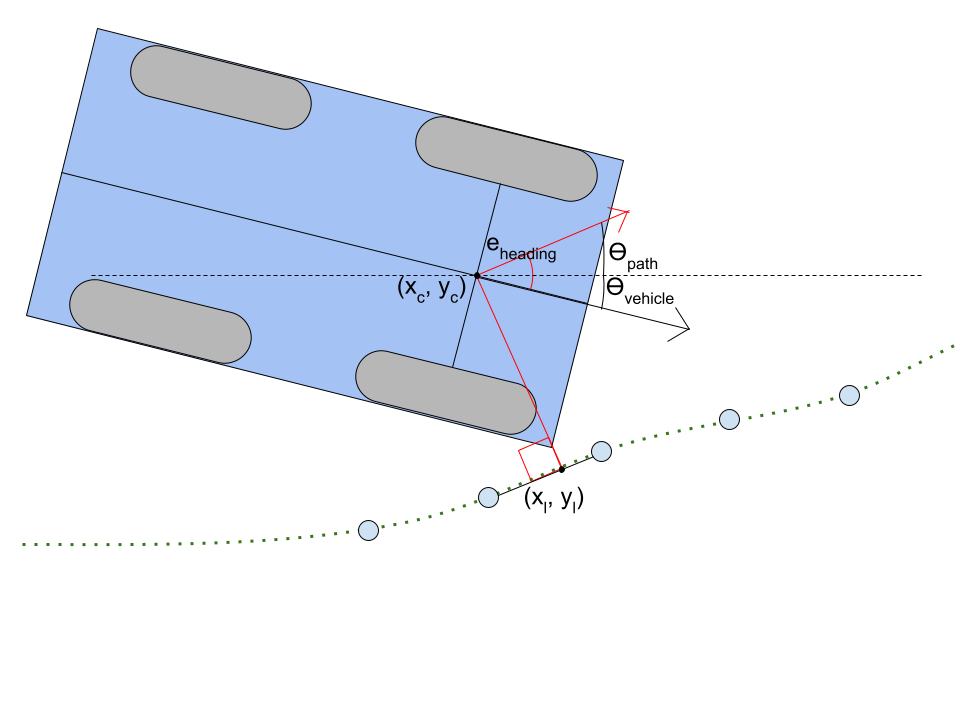
\includegraphics[width=5in]{stanley_heading_error}
	\caption{Calculation of the Heading Error for the Stanley Controller}
	\label{fig:stanley_heading_calc}
\end{figure}

Secondly, the cross track steering has to be configured. This is done by first identifying the cross track error, also known as the distance between the center of the front axis of the vehicle and the center of the lane. After the cross track error is calculated, it needs to be turned into a heading. The stanley controller uses the cross track error and calculates an angle by taking the inverse tangent of the ratio between the cross track error multiplied by a gain constant and the velocity of the vehicle. The result of this operation is the cross track heading, which is to be used as part of the final heading calculation. This calculation can be seen in Fig. \ref{fig:stanley_lateral_calc}.

\begin{figure}
	\centering
	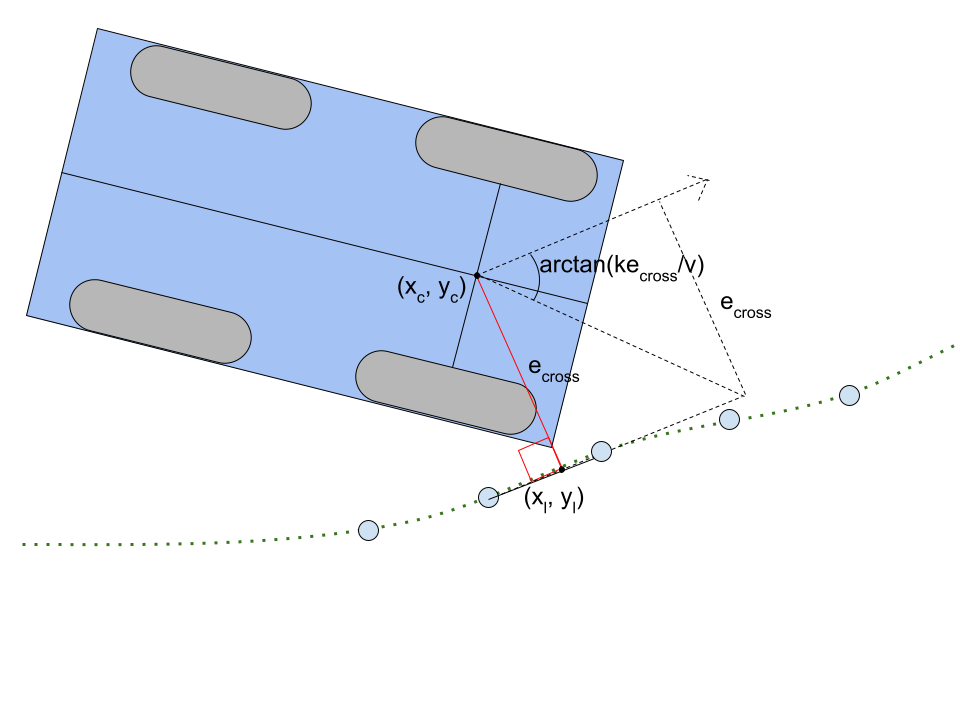
\includegraphics[width=5in]{stanley_lateral_error}
	\caption{Calculation of the Lateral Error for the Stanley Controller}
	\label{fig:stanley_lateral_calc}
\end{figure}

After these two heading values have been determined, their values are added together to determine the final heading value for the current movement calculation.

Another important part of the output command is the output velocity. The AckermannDrive requires a target speed to achieve, so another mechanism has to be put in place to determine which speed should be used. For our system, we decided that a PID controller should be effective for managing the velocity of the controls, but in order to keep things as simple as possible to reduce the amount of issues no controller was implemented for the longitudal control and only the lateral controllers were used.
\\

\underline{Evaluating the Stanley Controller}

After the controller was implemented, necessary procedures had to be created in order to properly evaluate the controller. Since at this point in time only CARLA has been properly integrated, a means of evaluating the performance of the controller though CARLA had to be used. Fortunately, within CARLA is as series of waypoints that are generated whenever a vehicle spawns into a map. Those waypoints can be taken and then modified to be fed into the control system as a means of providing a path without the detection module by providing those waypoints in a form similar to the way lanes are presented to the subsystem. In order to send the right waypoints, a new evaluation subsystem was designed that listens to CARLA for the vehicles current position in the map which then generates a series of points which is then sent to the vehicle. Furthermore, since this subsystem can listen to the vehicles position at all times, it is able to output graphs detailing the path of the vehicle as it travels through the system, and with the waypoints being followed identify how far away from the center of the road the vehicle is at all times. The visualizations for the vehicle were created with pythons MatPlotLib package.

\subsubsection{Evaluation}
\textbf{Evaluating FR2}

When it comes to evaluating the subsystem, the most important requirement for the quality of the control system is the maximum lateral error, also known as the maximum deviation from the center of the lane.

The methodology used for evaluating this functional requirement was primarily done through the evaluation subsystem described in the prior subsection. The vehicle was spawned at a specific point on the Town04 map, and follows a set of waypoints. These path chosen was due to the shape of its path. The path starts off with a shallow snaking patter, followed by a wide left turn. Afterwards, there is a straight section where the vehicle goes up a hill. Then, the vehicle performs a loop similar to the ones seen on a cloverleaf highway interchange. Lastly, the vehicle performs a sharp right hand turn.

Once the vehicle gets within 5 meters of the last waypoint, the evaluation subsystem will generate three figures: one overlaying the vehicle's path with the waypoint path, one illustrating the vehicles cross track error over time, and one illustrating the vehicles heading error over time. Additionally, each execution of the test will also output the maximum heading error the vehicle exhibited as well as the maximum lateral error the vehicle exhibited in order to identify whether the requirements have been achieved. This test will be repeated nine times, each with a unique combination of the stanley controller's 'k' control constant, which effects how far the control system "looks ahead" when calculating the cross track heading, and the standing velocity of the vehicle. The three different 'k' values that will be used are \texttt{0.5 1/s}, \texttt{1.0 1/s}, and \texttt{1.5 1/s}. The three different standing velocities used will be \texttt{4.0 m/s}, \texttt{6.0 m/s}, and \texttt{8.0 m/s}. The results of the nine tests can be seen in Table \ref{tab:controller_test_values}

\begin{table}
	\centering
	\begin{tabular}{| c | c | c | c |}
		\hline
		k (1/s) & Velocity (m/s) & max lateral error (meters) & max heading error (rads) \\ [0.5ex]
		\hline
		0.5     & 4.0            & 2.504                      & 0.6159                   \\
		\hline
		0.5     & 6.0            & 3.620                      & 0.6102                   \\
		\hline
		0.5     & 8.0            & 5.121                      & 0.5884                 \\
		\hline
		1.0     & 4.0            & 2.190                      & 0.5328                   \\
		\hline
		1.0     & 6.0            & 3.698                      & 0.6457                   \\
		\hline
		1.0     & 8.0            & 4.603                      & 0.6187                   \\
		\hline
		1.5     & 4.0            & 2.110                      & 0.4450                   \\
		\hline
		1.5     & 6.0            & 3.550                      & 0.6637                   \\
		\hline
		1.5     & 8.0            & 4.665                      & 0.5294                   \\
		\hline
	\end{tabular}
	\caption{Results of the Maximum Heading and Lateral Error for Various K and Speed Values}
	\label{tab:controller_test_values}
\end{table}

The results of the testing identified that the best performance for both maximum lateral error and maximum heading error was achieved when the k value was equal to \texttt{1.5 1/s} and the standing velocity was equal to \texttt{4.0 m/s}. Unfortunately, this result failed to reach the functional requirement of having a maximum lateral error of \texttt{0.45 meters}. The full path that the vehicle took can be seen in Fig.\ref{fig:waypointsk10v4}, the graph of the lateral error can be seen in Fig\ref{fig:lateralk10v4}, and the heading error of the trial can be seen in Fig\ref{fig:headingk10v4}. The figures depicting the path, lateral error, and heading error for the remaining 8 trials can be found in the appendix.

\begin{figure}
	\centering
	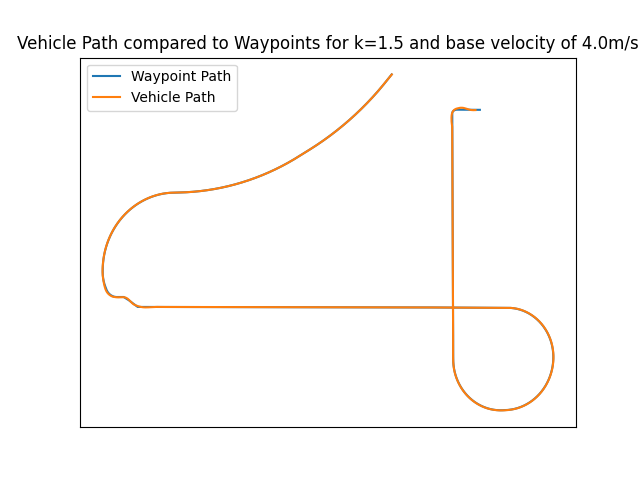
\includegraphics[width=4in]{/knc_eval/waypoints_k-15_v-4}
	\caption{Vehicle Path Compared to Waypoints for k=1.5 1/s and Base Velocity of 4.0 m/s Over Time}
	\label{fig:waypointsk10v4}
\end{figure}

\begin{figure}
	\centering
	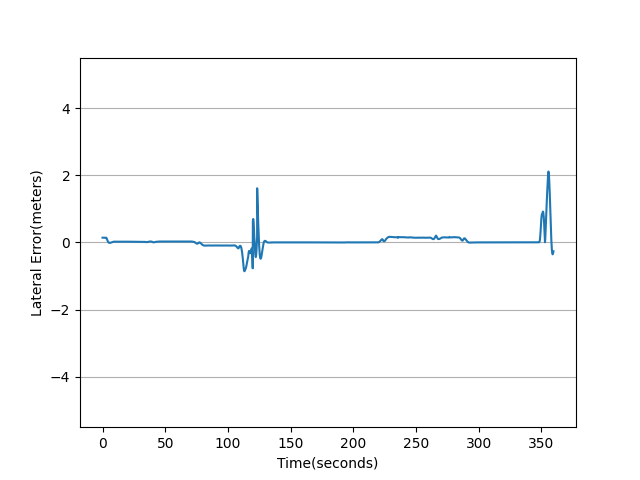
\includegraphics[width=4in]{/knc_eval/lateral_k-15_v-4}
	\caption{Lateral Error with k=1.5 1/s and Base Velocity of 4.0 m/s Over Time}
	\label{fig:lateralk10v4}
\end{figure}

\begin{figure}
	\centering
	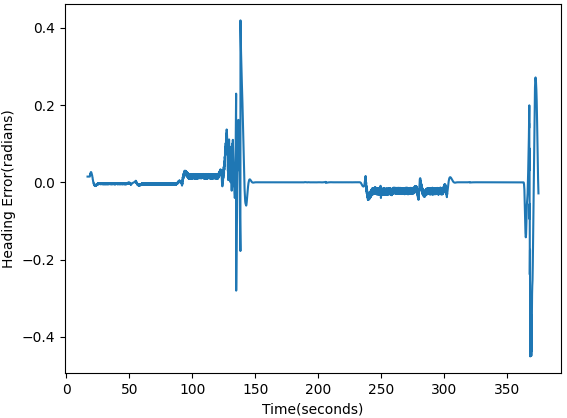
\includegraphics[width=4in]{/knc_eval/heading_k-15_v-4}
	\caption{Heading Error with k=1.5 1/s and Base Velocity of 4.0 m/s Over Time}
	\label{fig:headingk10v4}
\end{figure}

Upon further analysis of the figures, it can be identified that there were only two instances where the vehicle deviated beyond the required \texttt{0.45 meters} maximum deviation. When compared to the path of the vehicle, it can be identified that these two instances occurred when the vehicle was performing the left-hand turn approximately 35\% of the way through the course and the sharp right-handed turn at the end of the path. If these two instances are removed, the vehicle demonstrates a strong ability to stay within the requirement of a maximum lateral error of \texttt{0.45 meters}. However, these two cases are important for evaluating the lane following of the vehicle as sharp turns in a road can appear and the vehicle must be ready for them.

Additionally, it should be noted that all tests were performed a singular time. For a better performance evaluation, additional tests should be used to calculate a proper confidence interval.

\textbf{Evaluating FR2.1}

The evaluation for determining whether FR2.1 was satisfied comes down to the maximum heading error. There are many different ways to interpret what stability is represented by in the vehicle, but for our system we defined stability as the maximum heading error that the vehicle exhibits during a drive. As a team, we decided that the maximum heading error for our vechicle should be a 22.5 degree angle, or \(\pi/8\) radians in order to satisfy this requirement. This is not based on any actual calculation, but rather is an estimate as to the largest possible heading error a vehicle could have at the center of the land without exiting the lane.

In order to evaluate this requirement, the same methodology as FR2 was performed. The vehicle was spawned at a specific point on the Town04 map, and follows a set of waypoints. As before, the path was chosen because the path exhibits a wide range of steerings that would be useful for assessing the performance of the subsystem. The results for this test have been included in the evaluation for FR2, as both requirements were performed at the same point in time.

The results of the test found that even with the best possible configuration of standing velocity and control constant, the lowest heading error occurred with a k value of \texttt{1.5 1/s} and the standing velocity was equal to \texttt{4.0 m/s} with a maximum heading error of 0.4508 radians. Unfortunately, this also falls short of the requirement for this section.

A closer look at the heading error chart demonstrates as well that for a vast majority of the vehicles path the heading error remains very low, and only becomes much larger as the vehicle approaches much sharper turns. As a result, future work on this domain should be placed on improving the quality of the land following when sharper turns are present as this appears to be the most difficult part for the system to achieve.


\textbf{Evaluating FR2.2}

Another important requirement for this subsystem is the output frequency. This is important because the system must be able to output a sufficient number of movement commands each second in order to achieve the illusion of continuous driving.

Within our system, a timer within the control and keeping subsystem was configured to trigger the new movement output command on a variable frequency. This frequency is defined within the environmental variables of the command, and as a result it is very easy to adjust the frequency used internally. However, while it is possible that this value works we cannot be sure that this rate is actually achieved. If the amount of time it takes for the system to process a new request is longer than the soft deadline set by the timer, then the actual output frequency will not be the expected \(50Hz\). As a result, it is crucial for this to be tested experimentally to ensure that the proper frequency is actually being achieved by this.

The procedure by which this requirement was tested was through using a logger to output a log whenever a new movement command was outputted. Then, after increasing intervals of time the number of outputted logs will be analyzed and divided by the total time spent to achieve a frequency. The purpose of increased times is to get a better picture of what is actually happening as the longer the sample size, the less likely it is for smaller time segments to represent a biased part of the total population. The frequency observed after \(1s\), \(5s\), \(10s\), \(20s\), and \(60s\) can be observed in Table \ref{tab:frequency}.

\begin{table}
	\centering
	\begin{tabular}{| c | c | c |}
		\hline
		time (s) & Total Movement Commands Outputted & Movement Command Frequency \\ [0.5ex]
		\hline
		1.0      & 46                                & 46.00Hz                    \\
		\hline
		5.0      & 232                               & 46.40Hz                    \\
		\hline
		10.0     & 464                               & 46.40Hz                    \\
		\hline
		20.0     & 930                               & 46.50Hz                    \\
		\hline
		60.0     & 2787                              & 46.45Hz                    \\
		\hline
	\end{tabular}
	\caption{Results of the Maximum Heading and Lateral Error for Various K and Speed Values}
	\label{tab:frequency}
\end{table}


The results of this experiment show that at both long and short intervals of time, the output frequency of the system is approximately 46.4Hz. While this is not the required 50Hz frequency outlined in the functional requirements of the system, it is sufficiently close to the functional requirement to be considered achieved. This is in part due to the fact that the control system for this is not hard real time, and is instead soft real-time which means it is acceptable for the system to miss the occasional timer. As a result, this functional requirement has been achieved.

\textbf{Evaluating FR2.3}

One very important part of the system is the ability for the controller to be able to generate new movement commands using the latest availible data. This means that it must be able to interpret how far the vehicle has moved since the last image and predict where it currently is for the current movement command.

In order to evaluate this, the logs for the subsystem have to be observed. A log is posted each time a new set of lane data is given to the system, and a new log is also posted whenever a new movement command is posted. In order for this functional requirement to be satisfied, at least two movement commands must be uploaded between a pair of new lane data being provided and the two movement commands cannot be the same movement command. The results of this evaluation can be found in Fig. \ref{fig:fr23}.

\begin{figure}
	\centering
	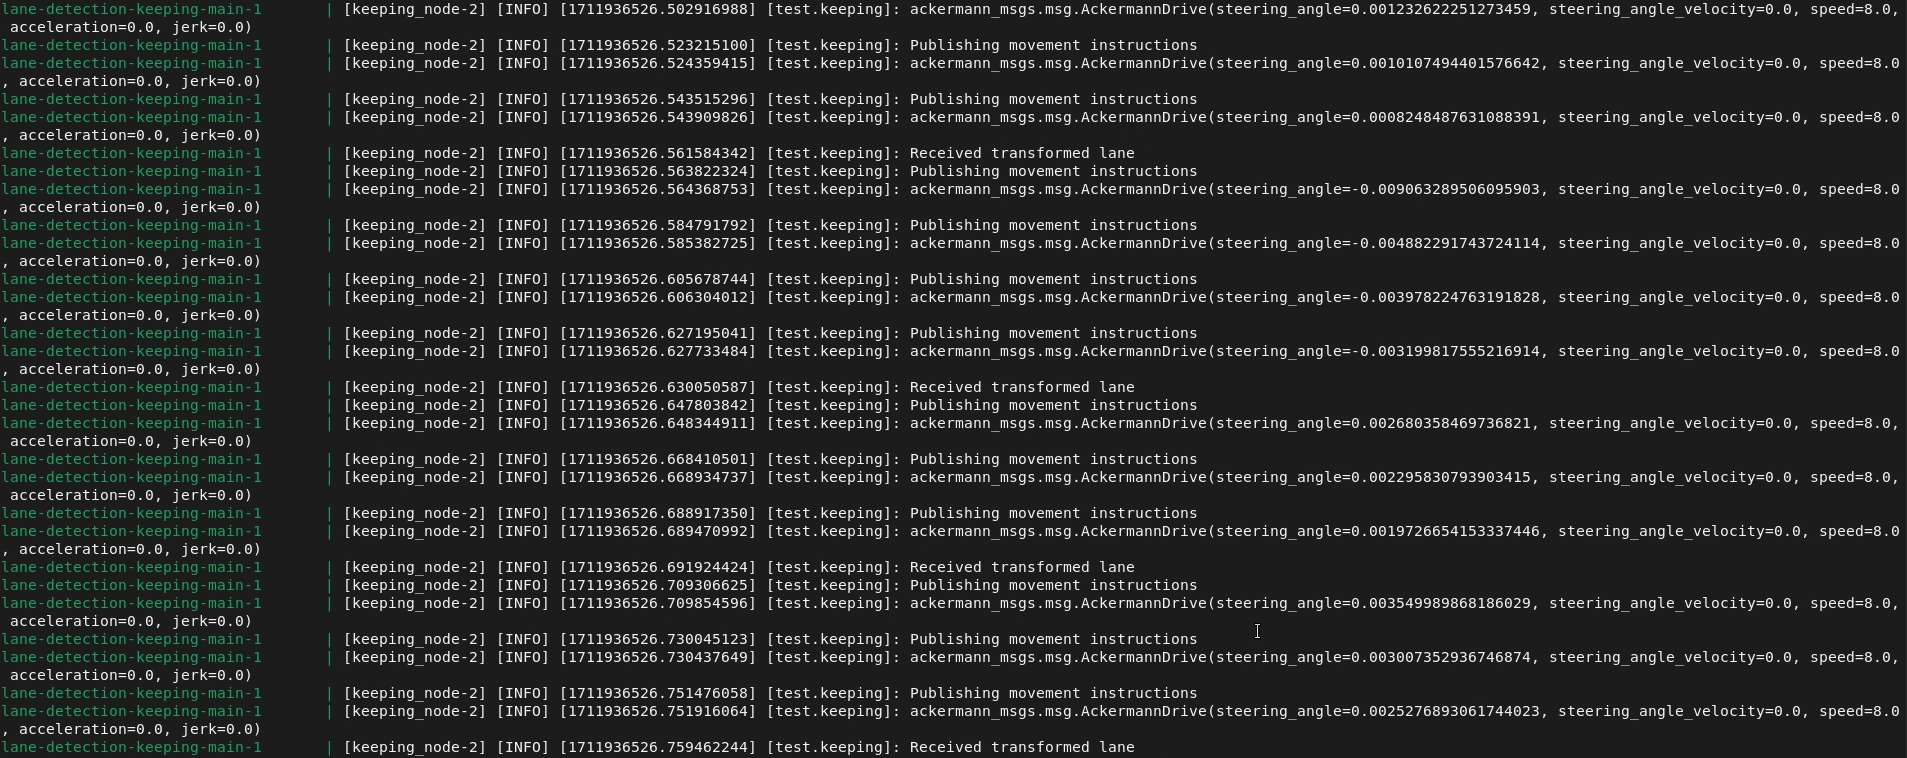
\includegraphics[width=6in]{fr23}
	\caption{Subset of Logs from the Keeping and Control Subsystem }
	\label{fig:fr23}
\end{figure}

The contents of the figure illustrate several instances between two lane being received logs where two or more movement commands were published, where each movement command was unique compared to the adjacent movement commands illustrating that the system exhibited closed loop properties and based movement commands on the latest available information, fulfilling the requirement.

\textbf{Evaluating FR2.4}
Our system outputs movement commands in the form of Ackermann messages, which are easily modifiable to fit any system requirement. Therefore, this requirement is fulfilled.


\section{System Integration and Evaluation}

\subsection{Integration}
Recall that the system is made up of two primary subsystems: Lane Detection and Lane Keeping \& Control. The Lane Detection subsystem processes real-time video camera footage from a vehicle as it drives, identifies lane markers and calculates the centre of the vehicle's lane. This information is relayed to the Keeping \& Control subsystem, which takes this data and determines the best corrective action to keep the vehicle centered in its lane. The K\&C subsystem is responsible for generating steering and acceleration commands based on the received lane position data, which is then sent to the vehicle hardware for execution.


\subsubsection{ROS2}
The Robot Operating System (ROS) is an open-source middleware suite for robotics. Despite its name, it is not an operating system but a software suite that runs mainly on Ubuntu. It provide a set of software frameworks for easy orchestration and data transfer between processes running on a robot.\cite{ros_documentation} Development on ROS 1 has ended and shifted to its successor, ROS 2, so we have chosen to use ROS 2 for orchestrating processes, facilitating data exchange and enabling interaction with the system's surrounding environment. Software using ROS follows a microservice architecture, with processes running as independent nodes that communicate with each other via messages sent through topics. Nodes can publish and subscribe to any number of topics, and topics can have any number of publishers and subscribers. When a node publishes a message to a given topic, all nodes subscribed to that topic receive the message. ROS is quite popular in the robotics industry, so there is good support for it from other software. CARLA, the simulation software we used, provides a bridge allowing it to communicate with ROS 1 and 2 nodes, publishing data such as a vehicle's camera feed to a topic and subscribing to a topic for movement commands.

ROS serves as the backbone of our system. Every subsystem runs as a set of ROS nodes that communicate with each other over a variety of topics. For example, the Lane Detection subsystem outputs the location of lanes to a specific topic, and the K\&C subsystem subscribes to that topic to get the data that it uses to determine what movement commands to send. Components of a subsystem work the same way. Inside Detection, for example, raw lines detected from the image are transformed to a top-down view before being sent to K\&C. Detecting the raw lines and transforming them are tasks done by different nodes, so the line data is passed between them on a topic. Because each step is a separate process, they do not all have to output at the same rate. K\&C, for instance, must output at a faster rate than Lane Detection to ensure steady operation of the vehicle at high speeds. For a given set of lanes sent to K\&C, it will send several commands before a new set of data arrives. This also allows parts of the system to handle faults more robustly. While not yet complete, work has begun on a Confidence component of Lane Detection that will take past lane data into account when sending data to K\&C, continuing to send confidently known lanes even if line detection fails to see them momentarily. This is all made very straightforward to orchestrate due to ROS 2, which handles all the details of message passing.

There are some downsides to using ROS, however. There are many different incompatible versions of ROS, and not all software supports all of them. ROS primarily targets running on Ubuntu, with other operating systems supported to varying extents. There is a different distro, or version, of ROS for every supported version of Ubuntu. For instance, ROS Melodic runs on Ubuntu 18.04, while ROS Noetic runs on Ubuntu 20.04. Different distros of ROS are not compatible, and sending messages between them is not officially supported in any capacity. Another divide exists between ROS 1 and ROS 2. ROS 2 is a newer version of ROS with many improvements, and aims to replace ROS 1 entirely. ROS 1 and 2 are not able to send messages to each other directly, but an official ROS bridge exists that can send messages between them so long as they are on the same version of Ubuntu. ROS 1 has mostly ended development, meaning no new distros will be released so it will never support any version of Ubuntu beyond 20.04. In May 2025 the last ROS 1 distro, Noetic, will be EOL. As such, we have chosen to use ROS 2 for our system. The downside to this is that the industry has not fully made the switch. There is much software out there that only supports ROS 1. Additionally, the CARLA ROS bridge mentioned earlier only supports ROS 2 Foxy, the ROS 2 distro targeting Ubuntu 20.04. The robot we used, however, runs ROS 1 Melodic on Ubuntu 18.04. This problem is described in more detail in the section on the HiWonder JetAcker.

Despite these issues, ROS provides huge benefits to the design and implementation of our system. It enables us to easily break down the system into separate subsystems and develop them independently of one another simultaneously. A simple stub can be made to publish test data, enabling easy testing of individual nodes. This makes splitting work between group members easy once topic names and message types are decided upon. It can make it harder to follow the flow of data, but since all nodes must subscribe to a topic using its name, a search in the codebase for the name of a topic will reveal all the nodes that publish and subscribe to it. Additionally, because nodes just publish to a topic without having to know what is subscribing to it, it is easy to swap out parts of the system by simply replacing them with a new node that publishes and subscribes to the same topics. This makes upgrading parts of the system or expanding it very easy. For instance, visualizing the data can be done by a node that simply subscribes to the relevant topics without having to make any other changes to the system. It also means that the system can easily be adapted to run on different hardware/simulations. All that is required is a node that can publish a camera feed to a topic and one that can control the hardware/simulation using the commands sent out by K\&C.

\begin{figure}[H]
	\centering
	\begin{minipage}{.45\textwidth}
		\centering
		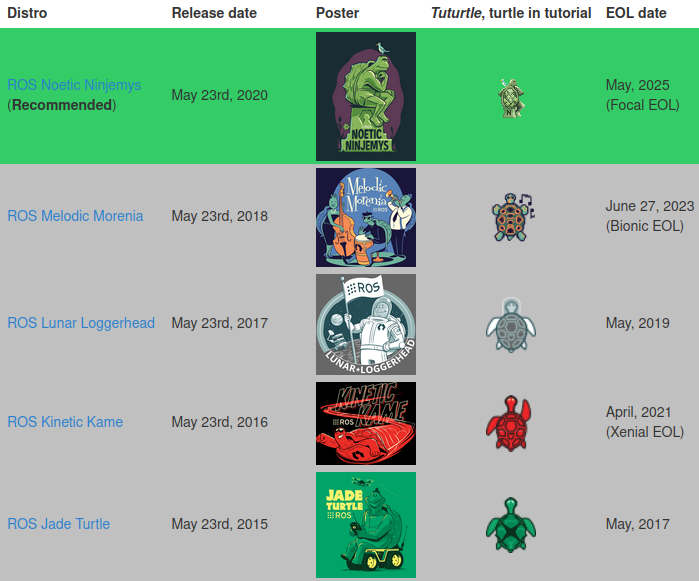
\includegraphics[width=\linewidth]{ROS1Distros.png}
		\captionof{figure}{A sample of ROS 1 distros from the ROS 1 wiki \cite{ROS1Distros}}
		\label{fig:ros1distros}
	\end{minipage}%
	\hspace{0.1\textwidth}%
	\begin{minipage}{.45\textwidth}
		\centering
		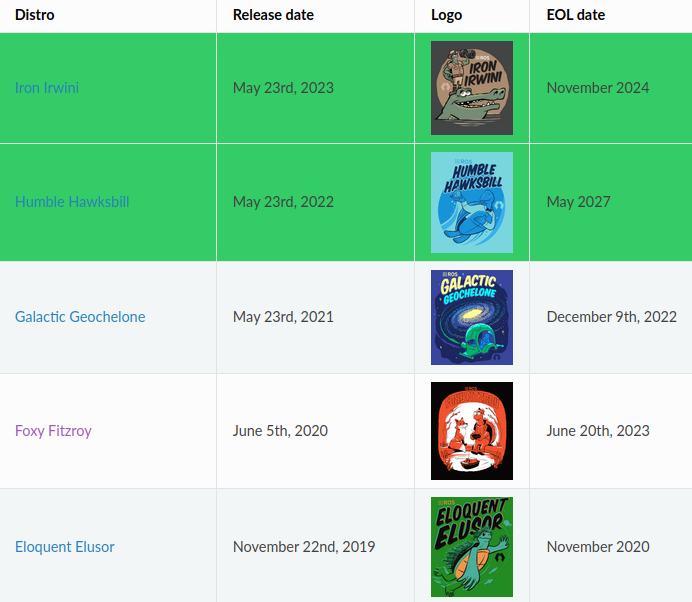
\includegraphics[width=\linewidth]{ROS2Distros.png}
		\captionof{figure}{A sample of ROS 2 distros from the ROS 2 wiki \cite{ROS2Distros}}
		\label{fig:ros2distros}
	\end{minipage}
\end{figure}

\subsubsection{Docker}
In addition to ROS, Docker was also used to assist with the integration of the software and hardware systems. A common problem with software is dependency issues, where running tasks would fail due to a dependency issue present with external packages. Docker solves this issue by making software run in isolated environments, making it less likely for packaging issues to be encountered. This helps with our project because there are a lot of dependency issues present with the simulation and the JetAcker, meaning containerized software is crucial to the applications success.


\subsection{Evaluation - Tools}
The system will be developed and evaluated for two phases of demonstration. The first phase will involve testing using a simulation environment, and the second will involve integration with a physical robot on a test roadway.

The evaluation of the individual Detection and K\&C subsystems will be completed as described in sections 3.1.6 and 3.2.6 respectively. The overall evaluation of the system will involve a more high level look at the system’s functionality.

\subsubsection{CARLA Simulator}
Our primary method of testing our system was CARLA, an open-source simulator for research on autonomous driving. CARLA provides a number of features vital to testing our system. It includes several detailed, realistic-looking maps. This is crucial for testing the Lane Detection subsystem, since the more realistic the simulation looks, the closer it is to a real road from the perspective of the car's camera. Too simple an environment may result in failure to properly evaluate the capabilities of the lane detection system. It also has realistic driving physics, crucial for testing the K\&C system. Furthermore, CARLA provides multiple maps with different types of roads, such as highways, suburban neighbourhoods, and city centers. This allowed us to test our system in many different environments and determine its strengths and weaknesses. Simulation of various weather conditions are also included, which is important since these are the situations in which autonomous driving systems struggle most.

Importantly, CARLA provides an interface to ROS 2 called the CARLA ROS Bridge. This bridge creates a few ROS 2 topics that CARLA publishes to, providing data such as a video feed from a camera, the current speed of the car, and position relative to predefined waypoints on the map, as well as accepting movement commands. By connecting the inputs and outputs of our system to these topics, we were able to test our system in realistic conditions and evaluate its performance under close to real conditions.

TODO: Liam look at what I wrote (above) and add in some stuff about waypoints and evaluation in more detail.

For the main course of the project, testing will be performed in a simulation environment using CARLA. CARLA is a driving environment simulation tool used for iterative, test-driven development of autonomous driving systems.\cite{dosovitskiy2017carla} This testing method will give freedom of modifying the various parameters to be considered with respect to road conditions. Using the simulation will also allow for quick testing of features throughout development. When running simulations using CARLA, the distance from the centre of the lane will be determined by the detection subsystem and adjustments to remain in the lane will be made by the K\&C subsystem. The results of the adjustments will be observed and recorded to verify proper functioning of the system.

\subsubsection{HiWonder JetAcker}

\begin{figure}
	\centering
	\includegraphics*[width=0.4\textwidth]{JetAcker1}
	\caption{HiWonder JetAcker Autonomous Vehicle Robot.}
	\label{fig:JetAcker}
\end{figure}

Our secondary method for testing our system was intended to be the HiWonder JetAcker, a robot with an Ackermann steering geometry similar to that of a real car. Unfortunately, due to a fire that destroyed a different robot as well as the charger for the JetAcker, we were not able to run our system on the JetAcker. Much of the groundwork for doing so was completed just days before the fire.

The JetAcker is equipped with an RGB camera, a depth camera, and a LIDAR. Of these, we only planned to use the RGB camera. Its steering mechanism uses an Ackermann geometry in which the wheels used for steering rotate by different amounts in order to minimize slipping during a turn. This is the basis for the steering mechanisms used by real cars, which is why we chose to use the JetAcker. It provides us with a system that is controlled in much the same way as a real car.

Using the JetAcker proved to be much more difficult than expected, and numerous problems were encountered. The JetAcker was acquired around the halfway point of the project, and the hope was that our system would be able to easily integrate to any hardware due to its modular approach where only a video input and command output are required. The JetAcker, however, runs on ROS 1 Melodic on Ubuntu 18.04. Our system runs on ROS 2 Foxy on Ubuntu 20.04. There is a bridge for sending messages between ROS 1 and 2, but it only works for versions on the same version of Ubuntu. This meant that to send messages between our system and the JetAcker, we had to first bridge them from ROS 2 Foxy to ROS 1 Noetic, and then send them from Noetic to Melodic, and do the same in reverse to communicate the other way. The bridge is officially supported, but sending messages between different distros of ROS is unsupported for both ROS 1 and ROS 2. We found that Melodic and Noetic are capable of communicating, but it is not an ideal scenario since it is not supported officially.

Because our system is designed to operate on cars, we chose to use AckermannDrive messages for the control output. These messages contain a forward speed and a steering angle. This accurately reflects how steering a car works, as those are the variables that are physically controllable on a car. The same is true of the JetAcker, but its software is not capable of handling AckermannDrive messages, instead taking Twist messages containing a linear velocity and an angular velocity. We believe this is because the JetAcker was built using a different robot, the JetAuto, as a starting point, and the JetAuto has mecanum wheels that allow it to move and rotate independently and in any direction. Our choice to use AckermannDrive messages made using the ROS bridge much more difficult. By default, the ROS bridge only supports message types that are built into ROS. Twist is one of these, but AckermannDrive is not. To use message types that are not a part of ROS by default, the ROS bridge has to be built from source, which cannot be done without building ROS 2 from source first. Building ROS 2 from source is not a simple task, as it has many dependencies and is a huge project. Since the JetAcker runs Ubuntu 18.04 and we needed to bridge versions on Ubuntu 20.04, we built ROS 2 and the ROS Bridge in a Docker container running Ubuntu 20.04. Once the Dockerfile to create this container was finished, we were able to put it onto the JetAcker and build it. We then discovered that the JetAcker only has a few gigabytes of spare storage, so we had to replace the SD card on it to build the image. Once the image was built, we modified the source code of the JetAcker to allow it to respond to AckermannDrive messages, and tested that it worked. We were able to successfully control it with AckermannDrive messages sent from ROS 2 on a laptop connected to the JetAcker's wifi network.

Our plan was to construct a test track for the JetAcker in order to test our system in the real world. Having multiple environments to test our system, with different pros and cons, would have been incredibly useful. While the JetAcker is further from a real driving environment than CARLA, it is a physical machine, so it can provide valuable data that we could not get from CARLA.

\subsection{Evaluation - Results}

Due to the complications that arose with the JetAcker, the primary method of evaluation for the system was done through the Carla simulation software. However, even though Carla is a great environment for testing there is a limited amount of information that can be extracted from the Carla-ROS bridge that makes it difficult to evaluate where the lane centre truly is. In order to get around this, the waypoint path that was used for the keeping and control subsystem was broken into four distinct parts that each exhibited a unique path characteristic that can be used to evaluate the system as a whole. The vehicle is then spawned at the beginning of each segment, and once the vehicle reaches the end the evaluation subsystem will output the maximum lateral error and the error over time associated with that trial.

The four different trial paths used for the evaluation are a straight line, a shallow snake curve, a moderately sharp circular curve, and a straight line that has a lane merge. The straight line is a path that has no turns associated with it, and it meant to confirm that the vehicle is actually capable of following a clear path. The second evaluation path is the shallow snake path. The purpose of this path is to determine that the vehicle is capable of identifying curves present in the vehicles field of view, and then to then proceed to follow the lanes. The two curves in the snake path have a radii of approximately 340 meters and 85 meters, respectively. Thirdly, a moderately sharp circular path was added to evaluate if the vehicle can control itself well on sharper corners. The curve of the circular shape has a radius of approximately 55 meters. Lastly, a straight lane path that has another lane merge into it was used to evaluate how the system is able to handle that scenario.

Each trial path was run through five times to achieve an average maximum lateral error over time. Additionally, each trial path outputted a line chart of the lateral error over time to identify any noticeable patterns present in the lateral error. Finally, each trial also outputted a line chart comparing the overall path of the vehicle to the path of the waypoints to provide a birds-eye view of the path the vehicle takes. The results of the testing can be found in Table \ref{tab:overal_eval}.

\begin{table}[H]
	\centering
	\begin{tabular}{c c c c c c c c }
		\textbf{Trial Path} & \textbf{Trial 1} & \textbf{Trial 2} & \textbf{Trial 3} & \textbf{Trial 4} & \textbf{Trial 5} & \textbf{Average} & \textbf{Standard Deviation} \\ [0.5ex]
		\hline
		Straight Path & 0.0529 m & 0.0405 m & 0.0491 m & 0.0573 m & 0.0535 m & 0.0506 m & 0.0064 m \\		
		\hline
		Snake Path & 0.3216 m & 0.3174 m & 0.3202 m & 0.3172 m & 0.3223 m & 0.3197 m & 0.0023 m \\		
		\hline
		Circle Path & 0.5086 m & 0.4997 m & 0.5119 m & 0.5104 m & 0.5455 m & 0.5152 m & 0.0176 m \\		
		\hline
		Merge Path & 1.4733 m & 1.3943 m & 1.4385 m & 1.4829 m & 1.4563 m & 1.4491 m & 0.0350 m \\		
		\hline
	\end{tabular}
	\caption{Results of Maximum Lateral Devation across 5 Trials for 4 Unique Paths}
	\label{tab:overal_eval}
\end{table}

\textbf{Straight Path}

The straight path had little relevant insights to gain from it. The average maximum lateral error for this path was 0.0535 meters, which is well below the maximum lateral error threshold defined in Functional Requirement 2. Further analysis of the lateral error over time graphs does not highlight anything of note, as the lateral error remains too low to show anything meaningful as seen in Fig. \ref{fig:straight_lat_1}. Furthermore, a review of the vehicle path compared to the waypoint path demonstrates that there is almost a complete overlap between the vehicles path and the waypoints. Therefore, in the case of a completely straight path the system can maintain a maximum lateral heading below 0.45 meters.

\begin{figure}
	\centering
	\begin{minipage}{.45\textwidth}
		\centering
		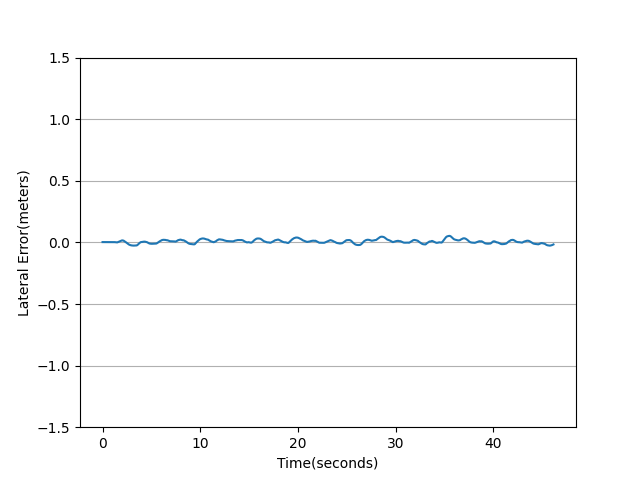
\includegraphics[width=\linewidth]{/overall_eval/lateral_straight_1}
		\caption{Lateral error over time for straight path trial 1}
		\label{fig:straight_lat_1}
	\end{minipage}%
	\hspace{0.1\textwidth}%
	\begin{minipage}{.45\textwidth}
		\centering
		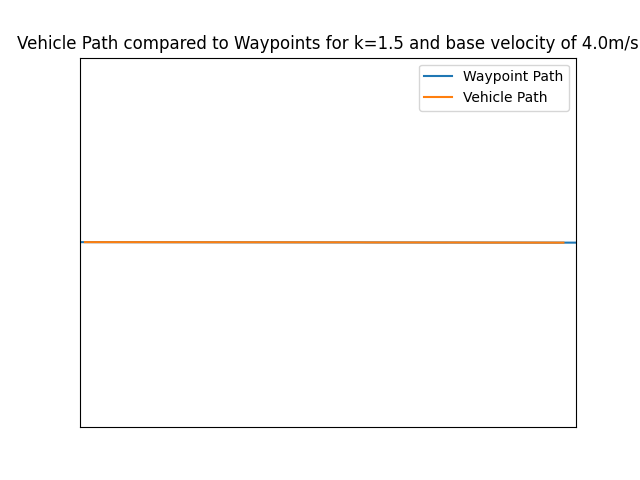
\includegraphics[width=\linewidth]{/overall_eval/waypoints_straight_1}
		\caption{Top-down view of vehicle path compared to lane center for straight path trial 1}
		\label{fig:straight_way_1}
	\end{minipage}
\end{figure}

\textbf{Snake Path}

The snake path was originally chosen to evaluate how effectively the autonomous driving system can deal with the existence of turns in the road in each direction. For this trial, the vehicle achieved an average maximum lateral error of 0.3457 meters, which while it is close to the maximum lateral error of 0.45 meters it still remains acceptable. Upon further investigation of the lateral error over time graph found at Fig. \ref{fig:snake_lat_1} in conjunction with the vehicle path graph found at Fig. \ref{fig:snake_way_1}, a few key points can be identified. For starters, the two halves of the vehicle path can be identified. The first half of the snake shape was a lot more shallow than the second half, which resulted in an average lateral error that visually appears around half of what was seen in th second half. Furthermore, The moment when the vehicle switches the direction of the curve there is a noticeable peak in the lateral error before the vehicle finds its footing and has a more steady lateral error. This increased initial error is likely due to the vehicle not responding quickly enough to the curvature of the path, and as a result it accidentally overshoots. All that said, in the case of a slightly curved path in both direction the system can maintain a maximum lateral heading below 0.45 meters.

\begin{figure}
	\centering
	\begin{minipage}{.45\textwidth}
		\centering
		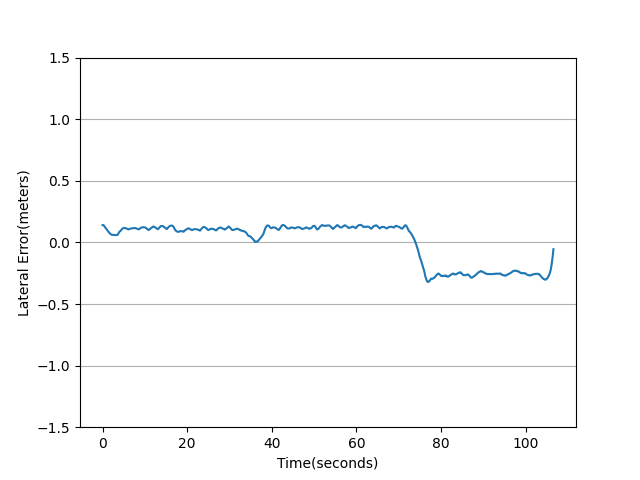
\includegraphics[width=\linewidth]{/overall_eval/lateral_snake_1}
		\captionof{figure}{Lateral Error over Time for Snake Path Trial 1}
		\label{fig:snake_lat_1}
	\end{minipage}%
	\hspace{0.1\textwidth}%
	\begin{minipage}{.45\textwidth}
		\centering
		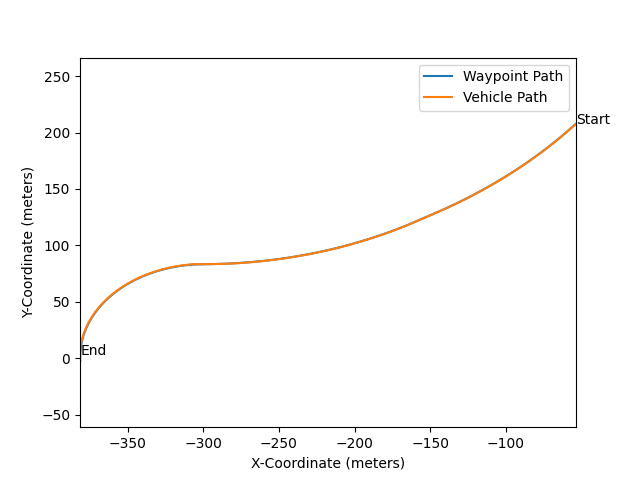
\includegraphics[width=\linewidth]{/overall_eval/waypoints_snake_1}
		\captionof{figure}{Vehicle Path compared to Lane Center for Snake Path Trial 1}
		\label{fig:snake_way_1}
	\end{minipage}
\end{figure}

\textbf{Circle Path}

The third trial map our team chose was the Circle path, which was originally chosen to evaluate how effectively the autonomous driving system can deal with sharper turns. For this trial, the vehicle achieved an average maximum lateral error of 0.5393 meters, which fails the requirement for maintaining a maximum lateral error below 0.45 meters. Upon further investigation of the lateral error over time graph found at Fig. \ref{fig:circle_lat_1} in conjunction with the vehicle path graph found at Fig. \ref{fig:circle_way_1}, a few notable patterns emerge. For starters, the same pattern observed with the snake path can be identified. When the vehicle begins on the track, it initially gets a very high lateral error which ends up being the maximum lateral error for the trial. However, this maximum lateral error is very quickly lowered to a more stable lateral error that does remain under the 0.45 meters identified in the requirements. As before, this is likely due to the initial overshoot of the vehicle not attempting to steer towards the lane centre at the beginning, but only after its already started moving away. However, while we can understand why this initial overshoot might be occurring the ability to handle this overshoot must exist in the lane evaluation system, and as a result in the case of a moderately curved path the system cannot maintain a maximum lateral heading below 0.45 meters.

\begin{figure}
	\centering
	\begin{minipage}{.45\textwidth}
		\centering
		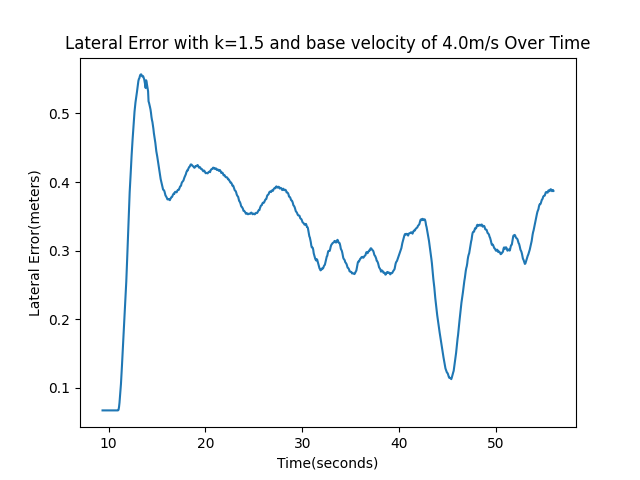
\includegraphics[width=\linewidth]{/overall_eval/lateral_circle_1}
		\captionof{figure}{Lateral Error over Time for Circle Path Trial 1}
		\label{fig:circle_lat_1}
	\end{minipage}%
	\hspace{0.1\textwidth}%
	\begin{minipage}{.45\textwidth}
		\centering
		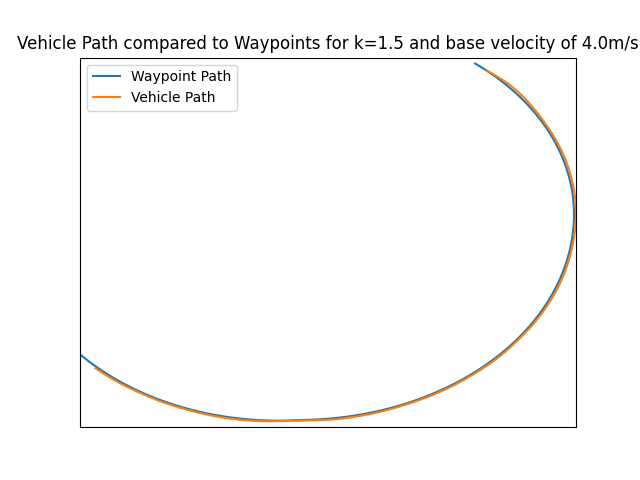
\includegraphics[width=\linewidth]{/overall_eval/waypoints_circle_1}
		\captionof{figure}{Vehicle Path compared to Lane Center for Circle Path Trial 1}
		\label{fig:circle_way_1}
	\end{minipage}
\end{figure}

\textbf{Merge Path}

The final trial that our team chose was a merge path. This means that the vehicle travels along a straight path, but partway through another lane merges into the current one and no line is visible for a short while. This is useful since a human driver would be able to identify the "invisible" lane line, and as a result the autonomous driving must as well. For this trial, the vehicle achieved a maximum lateral error of 1.4107 meters which falls well above the maximum lateral error tolerance defined in the requirements. Upon review of the lateral error over time graph found at Fig. \ref{fig:merge_lat_1} in conjunction with the vehicle path graph found at Fig. \ref{fig:merge_way_1}, it can be identified that the point at which the other lane merges into the vehicles lane the car fails to properly drive straight forward and instead veers to the side and takes a short amount of time to properly correct itself. Ultimately, in the case of a merging path into the vehicles current path the system cannot maintain a maximum lateral heading below 0.45 meters.

\begin{figure}
	\centering
	\begin{minipage}{.45\textwidth}
		\centering
		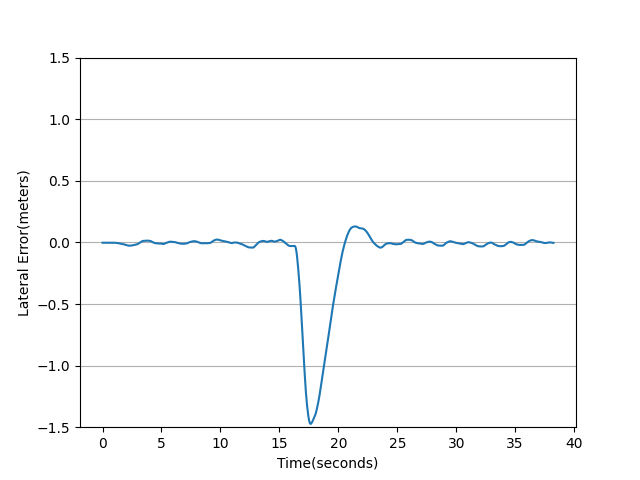
\includegraphics[width=\linewidth]{/overall_eval/lateral_merge_1}
		\captionof{figure}{Lateral Error over Time for Merge Path Trial 1}
		\label{fig:merge_lat_1}
	\end{minipage}%
	\hspace{0.1\textwidth}%
	\begin{minipage}{.45\textwidth}
		\centering
		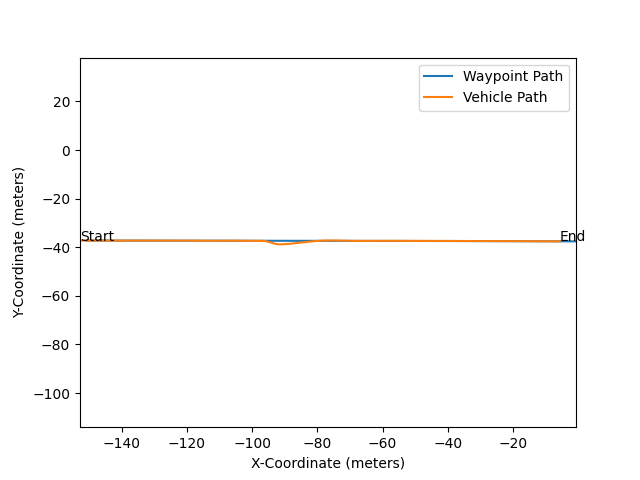
\includegraphics[width=\linewidth]{/overall_eval/waypoints_merge_1}
		\captionof{figure}{Vehicle Path compared to Lane Center for Merge Path Trial 1}
		\label{fig:merge_way_1}
	\end{minipage}
\end{figure}

\textbf{Conclusions}

Overall, the system was not capable of maintaining a maximum lateral error below 0.45 meters in all tested environments. It was capable of maintaining a sufficiently low maximum lateral error when the shape of curves in the road was sufficiently shallow, but after a certain point was no longer capable of always remaining between the lane lines. Furthermore, the system was incapable of keeping when any disturbances to the lane data were present since when the other lane merged onto the vehicles path it was incapable of properly determining the lane centre and flew off course.

Of further note, the other graphs generated in the other trials can be found in Appendix B.

\section{Reflections}

The final report needs to contain your original project proposal
(for example, as an Appendix or a separate chapter in your main
document). It is not uncommon that changes in your project goals
and objectives, methods used to achieve them, etc., may have
occurred over the course of the project. Therefore, in a final
chapter in the report, entitled “Reflections”, discuss how well
the original project objectives were met. Identify and discuss any
changes that occurred as the project progressed. Finally, as part
of this chapter, reflect, as a group, on the past two terms. Did
the project unfold as expected? Did the team work result in unexpected
challenges or benefits? With hindsight, if you had to undertake the
project again, would you make the same initial decisions about
tools/methods/timelines?

\subsection{Success of Project Objectives}

While we tried our best, we hit very few of our functional requirements for the system.

\subsection{Changes from Proposal}

WE had a lot of changes from our proposal.

While we wanted to make our own CNN, we were not able to make one on our own and had to instead use a pre-existing model.

While we initially planned to use a PID controller, it proved too complex and instead a mathematical model was used.

More...

\subsection{Group Reflection}

As a group, we believe that overall the project went very well.

\textbf{Project Unfolding as Expected}

The project ended up unfolding very differently from what we expected. Notably, we thought that a lot of parts would be much easier to learn than they actually were. At the start of the project, we did not have any extensive experience in the field of autonomous driving. As a result, any guess as to what we thought would happen was very inaccurate, with some actions taking significantly less time than expected and others taking significantly more time than expected. Furthermore, the focus of the project also shifted a lot between the proposal to the final product. At the beginning of the project, the focus was on designing an entirely new autonomous driving system using CARLA and the JetAcker as a means of testing the performance of the vehicle. However, as the project went on the team started to move away from creating the best possible autonomous driving system from scratch and instead worked towards creating an effective framework from which the autonomous driving system can be built from. The team spent a lot of time properly configuring Docker and ROS2 within the simulation environment so that a proper bridge between our system and CARLA can be used, with extensive documentation so that future groups can use our work in the future. Additionally, a lot of time was spent getting to the point where the JetAcker was in a state where it was possible for it to receive commands from an external computer. Combined, these two tasks took a significant portion of the development of the project.


\textbf{Unexpected Challenges and Benefits}

Since the project was a very new domain for everyone in the group, there was a rather large number of challenges that were faced over the course of the project.

For starters, a major initial challenge we encountered during the project was with the convolutional neural network. We initially planned to perform the lane detection by using our own neural network, but we were unable to actually design our own. It was a very ambitious attempt, but unfortunately we were not sufficiently proficient in that field to be able to even make a simple neural network from scratch. We were able to get around this by simply using an existing pre-trained neural network so we were able to get around the problem in the end.

Additionally, there were numerous challenges that took place in the development of the control system. Since no members of the team had any experience with control systems on account of the entire team being in the software engineering stream, we didn't know how to even start designing systems for that. This means one member of the team was effectively assigned to both learn and create a control system for use in the project. This presented with a wide range of challenges through almost every stage of learning.

On the hardware side, more stuff

\textbf{Decisions in Hindsight}

We bit off a lot more than we could chew. We're happy with the progress, but if we knew what we know now we would have been a lot more productive.

\vspace{12pt}

\appendix

\section{Keeping and Control Evaluation Graphs}
\label{FirstAppendix}

\begin{figure}[H]
	\centering
	\begin{minipage}{.45\textwidth}
		\centering
		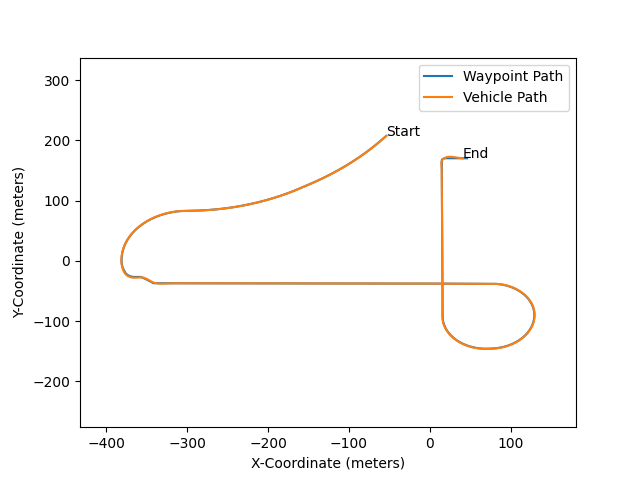
\includegraphics[width=\linewidth]{/knc_eval/waypoints_k-05_v-4.png}
		\captionof{figure}{Vehicle Path Compared to Waypoints for k=0.5 1/s and Base Velocity of 4.0 m/s Over Time}
		\label{fig:wayk5v4}
	\end{minipage}%
	\hspace{0.1\textwidth}%
	\begin{minipage}{.45\textwidth}
		\centering
		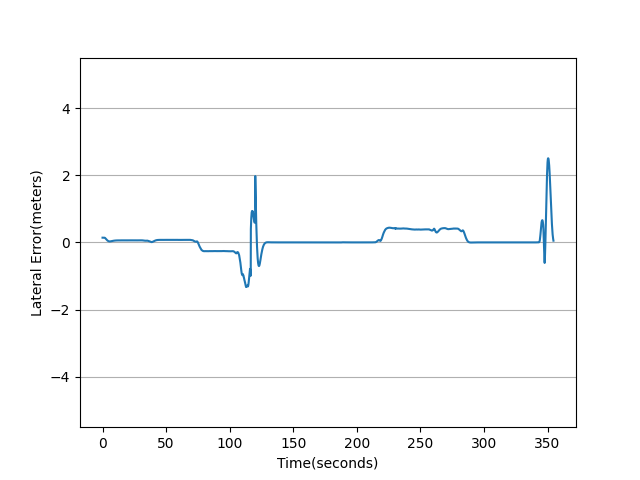
\includegraphics[width=\linewidth]{/knc_eval/lateral_k-05_v-4.png}
		\captionof{figure}{Lateral Error with k=0.5 1/s and Base Velocity of 4.0 m/s Over Time}
		\label{fig:latk5v4}
	\end{minipage}
\end{figure}

\begin{figure}[H]
	\centering
	\begin{minipage}{.45\textwidth}
		\centering
		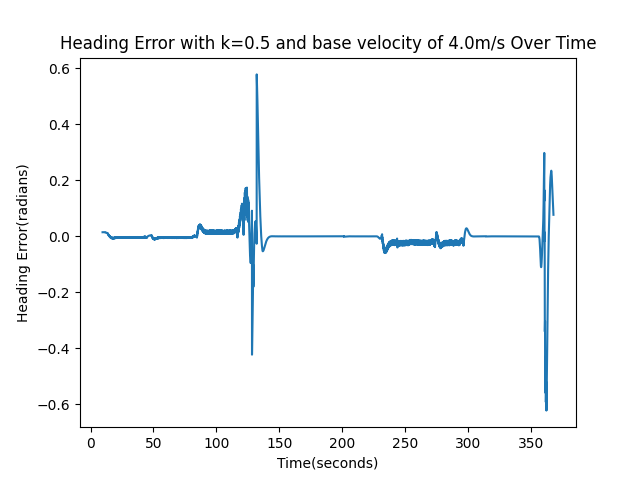
\includegraphics[width=\linewidth]{/knc_eval/heading_k-05_v-4.png}
		\captionof{figure}{Heading Error with k=0.5 1/s and Base Velocity of 4.0 m/s Over Time}
		\label{fig:headk5v4}
	\end{minipage}%
	\hspace{0.1\textwidth}%
	\begin{minipage}{.45\textwidth}
		\centering
		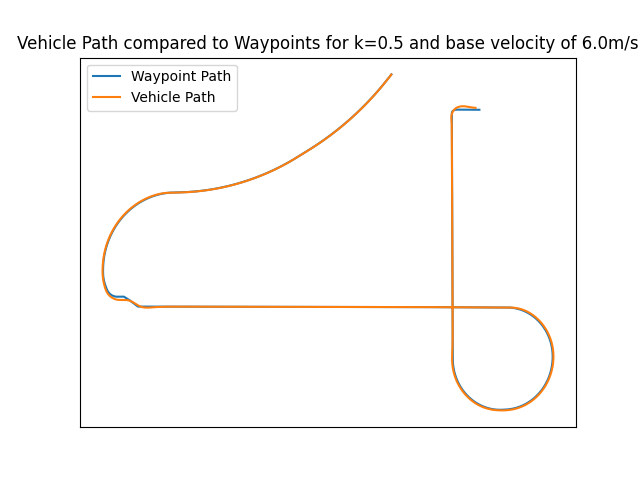
\includegraphics[width=\linewidth]{/knc_eval/waypoints_k-05_v-6.png}
		\captionof{figure}{Vehicle Path Compared to Waypoints for k=0.5 1/s and Base Velocity of 6.0 m/s Over Time}
		\label{fig:wayk5v6}
	\end{minipage}
\end{figure}

\begin{figure}[H]
	\centering
	\begin{minipage}{.45\textwidth}
		\centering
		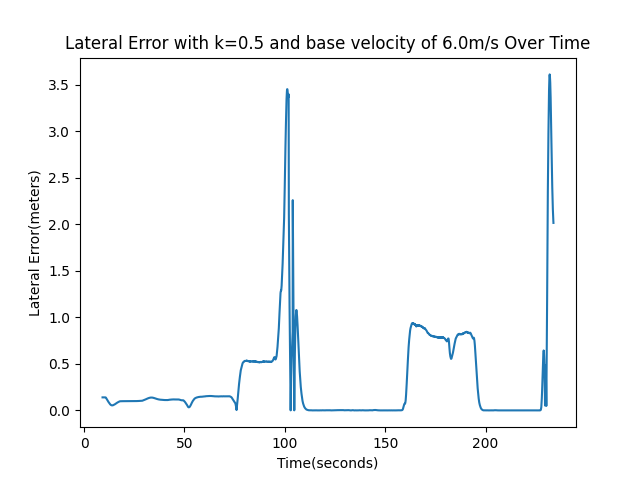
\includegraphics[width=\linewidth]{/knc_eval/lateral_k-05_v-6.png}
		\captionof{figure}{Lateral Error with k=0.5 1/s and Base Velocity of 6.0 m/s Over Time}
		\label{fig:latk5v6}
	\end{minipage}%
	\hspace{0.1\textwidth}%
	\begin{minipage}{.45\textwidth}
		\centering
		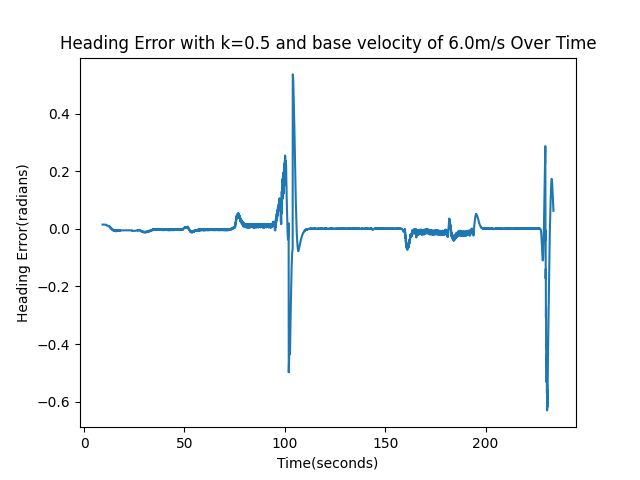
\includegraphics[width=\linewidth]{/knc_eval/heading_k-05_v-6.png}
		\captionof{figure}{Heading Error with k=0.5 1/s and Base Velocity of 6.0 m/s Over Time}
		\label{fig:headk5v6}
	\end{minipage}
\end{figure}

\begin{figure}[H]
	\centering
	\begin{minipage}{.45\textwidth}
		\centering
		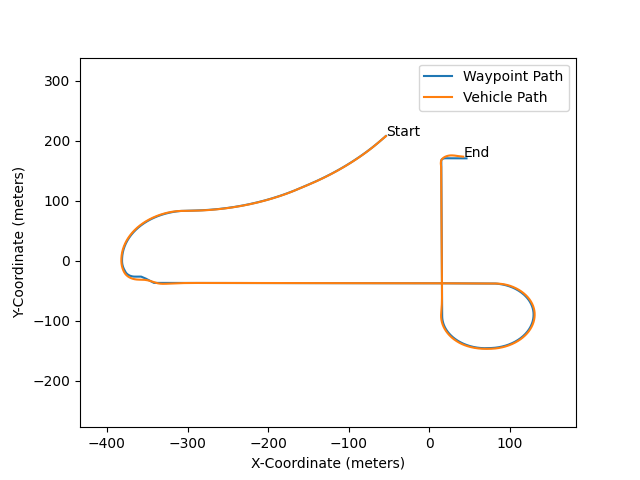
\includegraphics[width=\linewidth]{/knc_eval/waypoints_k-05_v-8.png}
		\captionof{figure}{Vehicle Path Compared to Waypoints for k=0.5 1/s and Base Velocity of 8.0 m/s Over Time}
		\label{fig:wayk5v8}
	\end{minipage}%
	\hspace{0.1\textwidth}%
	\begin{minipage}{.45\textwidth}
		\centering
		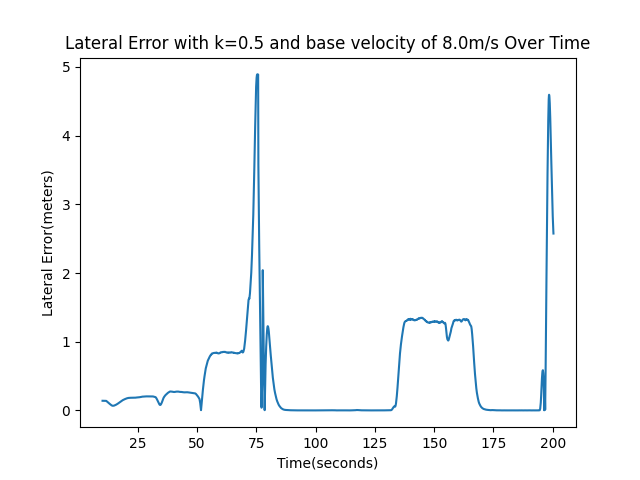
\includegraphics[width=\linewidth]{/knc_eval/lateral_k-05_v-8.png}
		\captionof{figure}{Lateral Error with k=0.5 1/s and Base Velocity of 8.0 m/s Over Time}
		\label{fig:latk5v8}
	\end{minipage}
\end{figure}

\begin{figure}[H]
	\centering
	\begin{minipage}{.45\textwidth}
		\centering
		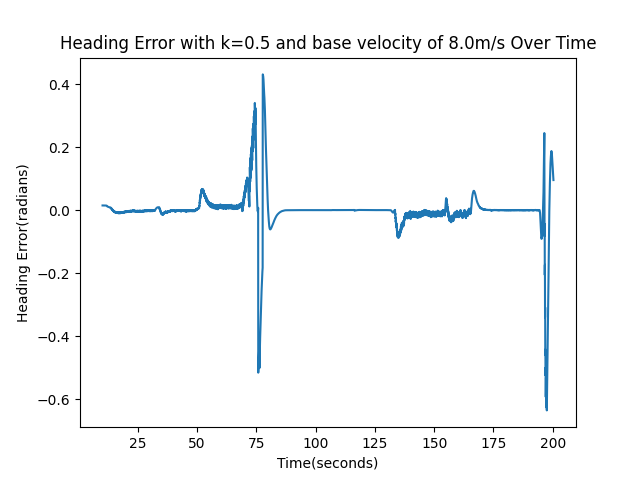
\includegraphics[width=\linewidth]{/knc_eval/heading_k-05_v-8.png}
		\captionof{figure}{Heading Error with k=0.5 1/s and Base Velocity of 8.0 m/s Over Time}
		\label{fig:headk5v8}
	\end{minipage}%
	\hspace{0.1\textwidth}%
	\begin{minipage}{.45\textwidth}
		\centering
		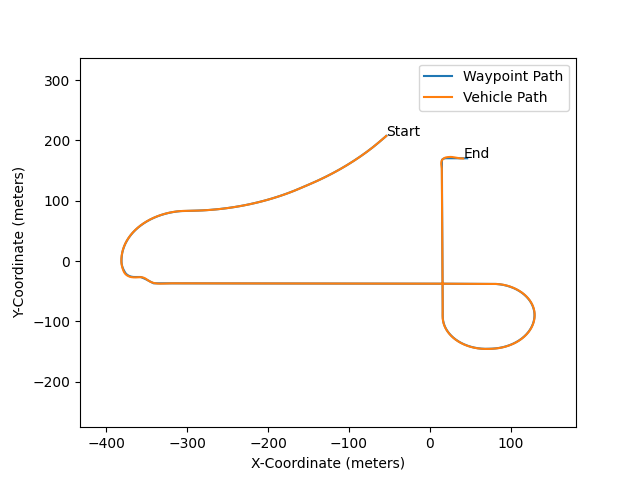
\includegraphics[width=\linewidth]{/knc_eval/waypoints_k-1_v-4.png}
		\captionof{figure}{Vehicle Path Compared to Waypoints for k=1.0 1/s and Base Velocity of 4.0 m/s Over Time}
		\label{fig:wayk10v4}
	\end{minipage}
\end{figure}

\begin{figure}[H]
	\centering
	\begin{minipage}{.45\textwidth}
		\centering
		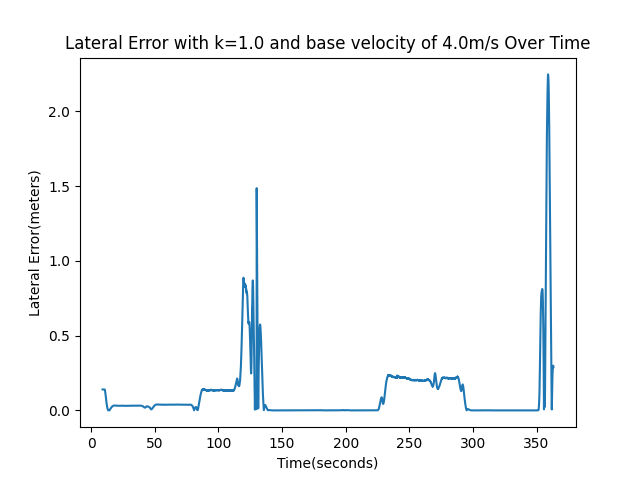
\includegraphics[width=\linewidth]{/knc_eval/lateral_k-1_v-4.png}
		\captionof{figure}{Lateral Error with k=1.0 1/s and Base Velocity of 4.0 m/s Over Time}
		\label{fig:latk10v4}
	\end{minipage}%
	\hspace{0.1\textwidth}%
	\begin{minipage}{.45\textwidth}
		\centering
		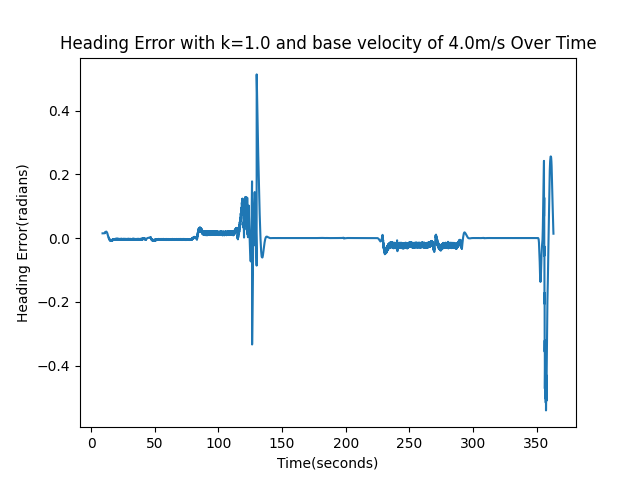
\includegraphics[width=\linewidth]{/knc_eval/heading_k-1_v-4.png}
		\captionof{figure}{Heading Error with k=1.0 1/s and Base Velocity of 4.0 m/s Over Time}
		\label{fig:headk10v4}
	\end{minipage}
\end{figure}


\begin{figure}[H]
	\centering
	\begin{minipage}{.45\textwidth}
		\centering
		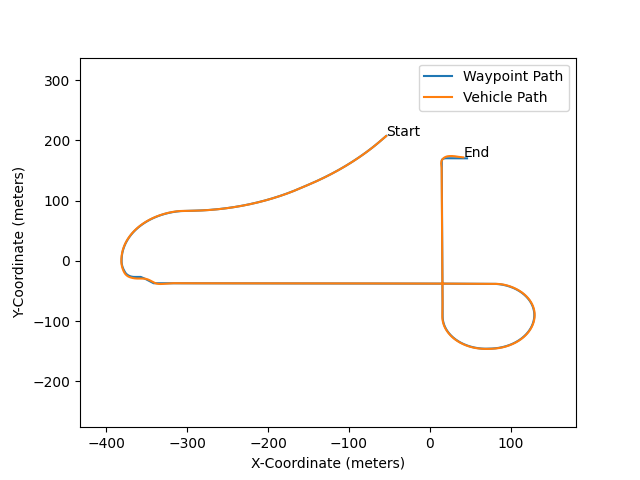
\includegraphics[width=\linewidth]{/knc_eval/waypoints_k-1_v-6.png}
		\captionof{figure}{Vehicle Path Compared to Waypoints for k=1.0 1/s and Base Velocity of 6.0 m/s Over Time}
		\label{fig:wayk10v6}
	\end{minipage}%
	\hspace{0.1\textwidth}%
	\begin{minipage}{.45\textwidth}
		\centering
		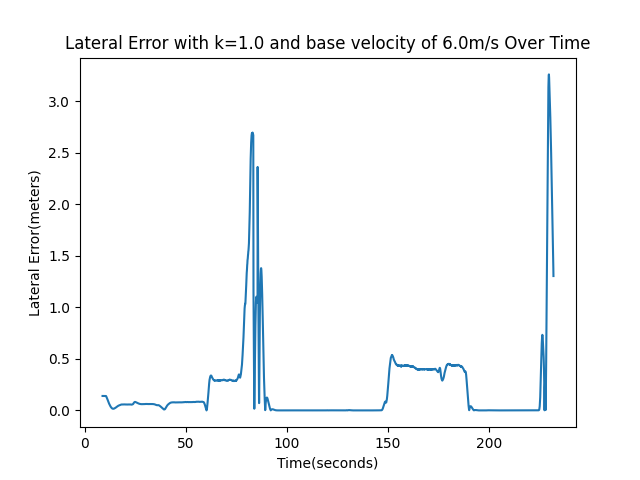
\includegraphics[width=\linewidth]{/knc_eval/lateral_k-1_v-6.png}
		\captionof{figure}{Lateral Error with k=1.0 1/s and Base Velocity of 6.0 m/s Over Time}
		\label{fig:latk10v6}
	\end{minipage}
\end{figure}

\begin{figure}[H]
	\centering
	\begin{minipage}{.45\textwidth}
		\centering
		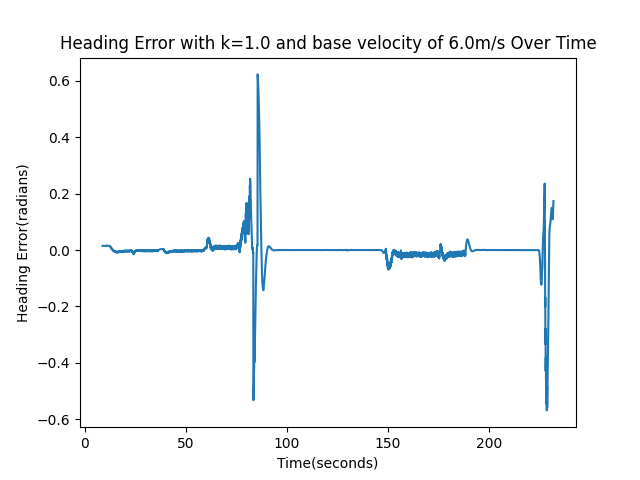
\includegraphics[width=\linewidth]{/knc_eval/heading_k-1_v-6.png}
		\captionof{figure}{Heading Error with k=1.0 1/s and Base Velocity of 6.0 m/s Over Time}
		\label{fig:headk10v6}
	\end{minipage}%
	\hspace{0.1\textwidth}%
	\begin{minipage}{.45\textwidth}
		\centering
		\includegraphics[width=\linewidth]{/knc_eval/waypoints_k-1_v-8.png}
		\captionof{figure}{Vehicle Path Compared to Waypoints for k=1.0 1/s and Base Velocity of 8.0 m/s Over Time}
		\label{fig:wayk10v8}
	\end{minipage}
\end{figure}

\begin{figure}[H]
	\centering
	\begin{minipage}{.45\textwidth}
		\centering
		\includegraphics[width=\linewidth]{/knc_eval/lateral_k-1_v-8.png}
		\captionof{figure}{Lateral Error with k=1.0 1/s and Base Velocity of 8.0 m/s Over Time}
		\label{fig:latk10v8}
	\end{minipage}%
	\hspace{0.1\textwidth}%
	\begin{minipage}{.45\textwidth}
		\centering
		\includegraphics[width=\linewidth]{/knc_eval/heading_k-1_v-8.png}
		\captionof{figure}{Heading Error with k=1.0 1/s and Base Velocity of 8.0 m/s Over Time}
		\label{fig:headk10v8}
	\end{minipage}
\end{figure}

\begin{figure}[H]
	\centering
	\begin{minipage}{.45\textwidth}
		\centering
		\includegraphics[width=\linewidth]{/knc_eval/waypoints_k-15_v-6.png}
		\captionof{figure}{Vehicle Path Compared to Waypoints for k=1.5 1/s and Base Velocity of 6.0 m/s Over Time}
		\label{fig:wayk15v6}
	\end{minipage}%
	\hspace{0.1\textwidth}%
	\begin{minipage}{.45\textwidth}
		\centering
		\includegraphics[width=\linewidth]{/knc_eval/lateral_k-15_v-6.png}
		\captionof{figure}{Lateral Error with k=1.5 1/s and Base Velocity of 6.0 m/s Over Time}
		\label{fig:latk15v6}
	\end{minipage}
\end{figure}

\begin{figure}[H]
	\centering
	\begin{minipage}{.45\textwidth}
		\centering
		\includegraphics[width=\linewidth]{/knc_eval/heading_k-15_v-6.png}
		\captionof{figure}{Heading Error with k=1.5 1/s and Base Velocity of 6.0 m/s Over Time}
		\label{fig:headk15v6}
	\end{minipage}%
	\hspace{0.1\textwidth}%
	\begin{minipage}{.45\textwidth}
		\centering
		\includegraphics[width=\linewidth]{/knc_eval/waypoints_k-15_v-8.png}
		\captionof{figure}{Vehicle Path Compared to Waypoints for k=1.5 1/s and Base Velocity of 8.0 m/s Over Time}
		\label{fig:wayk15v8}
	\end{minipage}
\end{figure}

\begin{figure}[H]
	\centering
	\begin{minipage}{.45\textwidth}
		\centering
		\includegraphics[width=\linewidth]{/knc_eval/lateral_k-15_v-8.png}
		\captionof{figure}{Lateral Error with k=1.5 1/s and Base Velocity of 8.0 m/s Over Time}
		\label{fig:latk15v8}
	\end{minipage}%
	\hspace{0.1\textwidth}%
	\begin{minipage}{.45\textwidth}
		\centering
		\includegraphics[width=\linewidth]{/knc_eval/heading_k-15_v-8.png}
		\captionof{figure}{Heading Error with k=1.5 1/s and Base Velocity of 8.0 m/s Over Time}
		\label{fig:headk15v4}
	\end{minipage}
\end{figure}

\section{System Evaluation Graphs}
\label{SecondAppendix}

\begin{figure}[H]
	\centering
	\begin{minipage}{.45\textwidth}
		\centering
		\includegraphics[width=\linewidth]{/overall_eval/lateral_straight_2}
		\captionof{figure}{Lateral Error over Time for Straight Path Trial 2}
		\label{fig:straight_lat_2}
	\end{minipage}%
	\hspace{0.1\textwidth}%
	\begin{minipage}{.45\textwidth}
		\centering
		\includegraphics[width=\linewidth]{/overall_eval/waypoints_straight_2}
		\captionof{figure}{Vehicle Path compared to Lane Center for Straight Path Trial 2}
		\label{fig:straight_way_2}
	\end{minipage}
\end{figure}

\begin{figure}[H]
	\centering
	\begin{minipage}{.45\textwidth}
		\centering
		\includegraphics[width=\linewidth]{/overall_eval/lateral_straight_3}
		\captionof{figure}{Lateral Error over Time for Straight Path Trial 3}
		\label{fig:straight_lat_3}
	\end{minipage}%
	\hspace{0.1\textwidth}%
	\begin{minipage}{.45\textwidth}
		\centering
		\includegraphics[width=\linewidth]{/overall_eval/waypoints_straight_3}
		\captionof{figure}{Vehicle Path compared to Lane Center for Straight Path Trial 3}
		\label{fig:straight_way_3}
	\end{minipage}
\end{figure}

\begin{figure}[H]
	\centering
	\begin{minipage}{.45\textwidth}
		\centering
		\includegraphics[width=\linewidth]{/overall_eval/lateral_straight_4}
		\captionof{figure}{Lateral Error over Time for Straight Path Trial 4}
		\label{fig:straight_lat_4}
	\end{minipage}%
	\hspace{0.1\textwidth}%
	\begin{minipage}{.45\textwidth}
		\centering
		\includegraphics[width=\linewidth]{/overall_eval/waypoints_straight_4}
		\captionof{figure}{Vehicle Path compared to Lane Center for Straight Path Trial 4}
		\label{fig:straight_way_4}
	\end{minipage}
\end{figure}

\begin{figure}[H]
	\centering
	\begin{minipage}{.45\textwidth}
		\centering
		\includegraphics[width=\linewidth]{/overall_eval/lateral_straight_5}
		\captionof{figure}{Lateral Error over Time for Straight Path Trial 5}
		\label{fig:straight_lat_5}
	\end{minipage}%
	\hspace{0.1\textwidth}%
	\begin{minipage}{.45\textwidth}
		\centering
		\includegraphics[width=\linewidth]{/overall_eval/waypoints_straight_5}
		\captionof{figure}{Vehicle Path compared to Lane Center for Straight Path Trial 5}
		\label{fig:straight_way_5}
	\end{minipage}
\end{figure}









\begin{figure}[H]
	\centering
	\begin{minipage}{.45\textwidth}
		\centering
		\includegraphics[width=\linewidth]{/overall_eval/lateral_snake_2}
		\captionof{figure}{Lateral Error over Time for Snake Path Trial 2}
		\label{fig:snake_lat_2}
	\end{minipage}%
	\hspace{0.1\textwidth}%
	\begin{minipage}{.45\textwidth}
		\centering
		\includegraphics[width=\linewidth]{/overall_eval/waypoints_snake_2}
		\captionof{figure}{Vehicle Path compared to Lane Center for Snake Path Trial 2}
		\label{fig:snake_way_2}
	\end{minipage}
\end{figure}

\begin{figure}[H]
	\centering
	\begin{minipage}{.45\textwidth}
		\centering
		\includegraphics[width=\linewidth]{/overall_eval/lateral_snake_3}
		\captionof{figure}{Lateral Error over Time for Snake Path Trial 3}
		\label{fig:snake_lat_3}
	\end{minipage}%
	\hspace{0.1\textwidth}%
	\begin{minipage}{.45\textwidth}
		\centering
		\includegraphics[width=\linewidth]{/overall_eval/waypoints_snake_3}
		\captionof{figure}{Vehicle Path compared to Lane Center for Snake Path Trial 3}
		\label{fig:snake_way_3}
	\end{minipage}
\end{figure}

\begin{figure}[H]
	\centering
	\begin{minipage}{.45\textwidth}
		\centering
		\includegraphics[width=\linewidth]{/overall_eval/lateral_snake_4}
		\captionof{figure}{Lateral Error over Time for Snake Path Trial 4}
		\label{fig:snake_lat_4}
	\end{minipage}%
	\hspace{0.1\textwidth}%
	\begin{minipage}{.45\textwidth}
		\centering
		\includegraphics[width=\linewidth]{/overall_eval/waypoints_snake_4}
		\captionof{figure}{Vehicle Path compared to Lane Center for Snake Path Trial 4}
		\label{fig:snake_way_4}
	\end{minipage}
\end{figure}

\begin{figure}[H]
	\centering
	\begin{minipage}{.45\textwidth}
		\centering
		\includegraphics[width=\linewidth]{/overall_eval/lateral_snake_5}
		\captionof{figure}{Lateral Error over Time for Snake Path Trial 5}
		\label{fig:snake_lat_5}
	\end{minipage}%
	\hspace{0.1\textwidth}%
	\begin{minipage}{.45\textwidth}
		\centering
		\includegraphics[width=\linewidth]{/overall_eval/waypoints_snake_5}
		\captionof{figure}{Vehicle Path compared to Lane Center for Snake Path Trial 5}
		\label{fig:snake_way_5}
	\end{minipage}
\end{figure}








\begin{figure}[H]
	\centering
	\begin{minipage}{.45\textwidth}
		\centering
		\includegraphics[width=\linewidth]{/overall_eval/lateral_circle_2}
		\captionof{figure}{Lateral Error over Time for Circle Path Trial 2}
		\label{fig:circle_lat_2}
	\end{minipage}%
	\hspace{0.1\textwidth}%
	\begin{minipage}{.45\textwidth}
		\centering
		\includegraphics[width=\linewidth]{/overall_eval/waypoints_circle_2}
		\captionof{figure}{Vehicle Path compared to Lane Center for Circle Path Trial 2}
		\label{fig:circle_way_2}
	\end{minipage}
\end{figure}

\begin{figure}[H]
	\centering
	\begin{minipage}{.45\textwidth}
		\centering
		\includegraphics[width=\linewidth]{/overall_eval/lateral_circle_3}
		\captionof{figure}{Lateral Error over Time for Circle Path Trial 3}
		\label{fig:circle_lat_3}
	\end{minipage}%
	\hspace{0.1\textwidth}%
	\begin{minipage}{.45\textwidth}
		\centering
		\includegraphics[width=\linewidth]{/overall_eval/waypoints_circle_3}
		\captionof{figure}{Vehicle Path compared to Lane Center for Circle Path Trial 3}
		\label{fig:circle_way_3}
	\end{minipage}
\end{figure}

\begin{figure}[H]
	\centering
	\begin{minipage}{.45\textwidth}
		\centering
		\includegraphics[width=\linewidth]{/overall_eval/lateral_circle_4}
		\captionof{figure}{Lateral Error over Time for Circle Path Trial 4}
		\label{fig:circle_lat_4}
	\end{minipage}%
	\hspace{0.1\textwidth}%
	\begin{minipage}{.45\textwidth}
		\centering
		\includegraphics[width=\linewidth]{/overall_eval/waypoints_circle_4}
		\captionof{figure}{Vehicle Path compared to Lane Center for Circle Path Trial 4}
		\label{fig:circle_way_4}
	\end{minipage}
\end{figure}

\begin{figure}[H]
	\centering
	\begin{minipage}{.45\textwidth}
		\centering
		\includegraphics[width=\linewidth]{/overall_eval/lateral_circle_5}
		\captionof{figure}{Lateral Error over Time for Circle Path Trial 5}
		\label{fig:circle_lat_5}
	\end{minipage}%
	\hspace{0.1\textwidth}%
	\begin{minipage}{.45\textwidth}
		\centering
		\includegraphics[width=\linewidth]{/overall_eval/waypoints_circle_5}
		\captionof{figure}{Vehicle Path compared to Lane Center for Circle Path Trial 5}
		\label{fig:circle_way_5}
	\end{minipage}
\end{figure}








\begin{figure}[H]
	\centering
	\begin{minipage}{.45\textwidth}
		\centering
		\includegraphics[width=\linewidth]{/overall_eval/lateral_merge_2}
		\captionof{figure}{Lateral Error over Time for Merge Path Trial 2}
		\label{fig:merge_lat_2}
	\end{minipage}%
	\hspace{0.1\textwidth}%
	\begin{minipage}{.45\textwidth}
		\centering
		\includegraphics[width=\linewidth]{/overall_eval/waypoints_merge_2}
		\captionof{figure}{Vehicle Path compared to Lane Center for Merge Path Trial 2}
		\label{fig:merge_way_2}
	\end{minipage}
\end{figure}

\begin{figure}[H]
	\centering
	\begin{minipage}{.45\textwidth}
		\centering
		\includegraphics[width=\linewidth]{/overall_eval/lateral_merge_3}
		\captionof{figure}{Lateral Error over Time for Merge Path Trial 3}
		\label{fig:merge_lat_3}
	\end{minipage}%
	\hspace{0.1\textwidth}%
	\begin{minipage}{.45\textwidth}
		\centering
		\includegraphics[width=\linewidth]{/overall_eval/waypoints_merge_3}
		\captionof{figure}{Vehicle Path compared to Lane Center for Merge Path Trial 3}
		\label{fig:merge_way_3}
	\end{minipage}
\end{figure}

\begin{figure}[H]
	\centering
	\begin{minipage}{.45\textwidth}
		\centering
		\includegraphics[width=\linewidth]{/overall_eval/lateral_merge_4}
		\captionof{figure}{Lateral Error over Time for Merge Path Trial 4}
		\label{fig:merge_lat_4}
	\end{minipage}%
	\hspace{0.1\textwidth}%
	\begin{minipage}{.45\textwidth}
		\centering
		\includegraphics[width=\linewidth]{/overall_eval/waypoints_merge_4}
		\captionof{figure}{Vehicle Path compared to Lane Center for Merge Path Trial 4}
		\label{fig:merge_way_4}
	\end{minipage}
\end{figure}

\begin{figure}[H]
	\centering
	\begin{minipage}{.45\textwidth}
		\centering
		\includegraphics[width=\linewidth]{/overall_eval/lateral_merge_5}
		\captionof{figure}{Lateral Error over Time for Merge Path Trial 5}
		\label{fig:merge_lat_5}
	\end{minipage}%
	\hspace{0.1\textwidth}%
	\begin{minipage}{.45\textwidth}
		\centering
		\includegraphics[width=\linewidth]{/overall_eval/waypoints_merge_5}
		\captionof{figure}{Vehicle Path compared to Lane Center for Merge Path Trial 5}
		\label{fig:merge_way_5}
	\end{minipage}
\end{figure}

\end{document}

% LocalWords:  leaderboard Ackermann JetAcker
